% This is a template for use with the MSU Thesis class
% Vesion 2.8 2017/12/13
%
% Class options: 
%[PhD]	Doctor of Philosophy (default) 
%[DEd]	Doctor of Education
%[DMA]	Doctor of Musical Arts
%[MA]	Master of Arts
%[MS]	Master of Science
%[MAT]	Master of Arts for Teachers
%[MBA]	Master of Business Administration
%[MFA]	Master of Fine Arts
%[MIPS]	Master of International Planning Studies
%[MHRL]	Master of Human Resources and Labor Relations 
%[MMus]	Master of Music
%[MPH]	Master of Public Health
%[MPP]	Master of Public Policy
%[MSW]	Master of Social Work
%[MURP]	Master in Urban and Regional Planning 
%%
% Default is PhD
%
%
% This template has everything in the right order.
% Just add real content and you're done!
%
\documentclass[]{msu-thesis}
%
% for a prettier, but possibly non-compliant table of contents use the [mixedtoc] option
% for a plain table of contents use the [plaintoc] option
% for a horrendous looking, but possibly required table of contents, use the [boldtoc] option
%
% If you have large tables/figures that need to be in landscape mode, add the [lscape] option

%IS THIS THE RIGHT BIB STYLE TO USE????!?!?!??!?!?!??!
%!!!!!!!!!!!!!!!!!!!!!!!!!!!!!!!!!!!!!!!!!!!!!!!
\bibliographystyle{elsarticle-num}

% This is standard fontenc/inputenc for pdflatex
% If you use LuaLaTeX or XeLaTeX you should replace this with the fontspec package
\usepackage[utf8]{inputenc}
\usepackage[T1]{fontenc}
\usepackage{float}
\usepackage{graphicx}
\graphicspath{{images/spacecharge/} {images/} }


%
% If the thesis office requires Times, we'll give them Times
% You can experiment with other font packages here if you like.
% If you are using XeLaTeX or LuaLaTeX load the Times or Times New Roman font with \setmainfont
\usepackage{newtxtext,newtxmath,booktabs,siunitx,caption,subcaption} 
%
% Load any extra packages here
%
% You must specify the title of your thesis, your name, the field of study (not department), and the year
\title{Constraining the High Density Nuclear Symmetry Energy with Pions}
\author{Justin Estee}
\fieldofstudy{Physics} % This should be in sentence case
\date{2019}

% If you want a dedication page, specify the text of the dedication here and uncomment the next command.
%
\dedication{This thesis is dedicated to someone.}
%

%User defined commands
\newcommand{\spirit}{S$\pi$RIT }
\newcommand{\ra}[1]{\renewcommand{\arraystretch}{#1}}
\includeonly{
%chapters/ch_intro,
%chapters/ch_theory,
chapters/ch_experiment,
chapters/ch_data_analysis,
%chapters/ch_data_analysis_2,
%chapters/ch_results
}


\begin{document}
%\sisetup{quotient-mode=fraction} % Output a/b as \frac{a}{b}

% All the stuff before your actual chapters is called the front matter
\frontmatter
% First make the title page
\maketitlepage
% Next make the abstract
\begin{abstract}
% Your abstract goes here.  Master's 1 page max. PhD 2 page max.
\end{abstract}

% Force a newpage
\clearpage
% Make the copyright page. The Graduate School ridiculously prohibits you
% from having a copyright page unless you pay ProQuest to register the copyright.
% This should be illegal, but I didn't make up the rule.

\makecopyrightpage

% If you have a dedication page, uncomment the next command to print the dedication page
%
%\makededicationpage
%
\clearpage
% Your Acknowledgements are formatted like a chapter, but with no number
\chapter*{Acknowledgements}
\DoubleSpacing % Acknowledgements should be double spaced
Your acknowledgements here.
%
\clearpage
% We need to turn single spacing back on for the contents/figures/tables lists
\SingleSpacing
\tableofcontents* % table of contents will not be listed in the TOC
\clearpage
\listoftables % comment this out if you have no tables
\clearpage
\listoffigures % comment this out if you have no figures
%
% If you have a list of abbreviations/symbols it would go here preceded by a \clearpage
% See the class documentation and the Memoir manual for how to create other lists 
%
\mainmatter
%
% The next line removes the dots in chapter headings in the TOC
% May violate thesis office rules
%\addtocontents{toc}{\protect\renewcommand{\protect\cftchapterdotsep} {\cftnodots}}

\chapter{Introduction}

Rutherford discovered in 1911 that the atomic nuclei are composed of a dense nucleus surrounded by an electron cloud, and eventually that the nucleus if composed of positive and neutral spin 1/2 particles called protons and neutrons. The proton and neutron are actually composed of 3 fundamental particles called quarks. Besides for the charge differences between protons and neutrons, they exhibit a fundamental symmetry which explains their almost identical mass. Typically neutrons and protons are treated as two different isospin projections of a ``nucleon", (-1/2 and 1/2) respectively.



The nucleus itself accounts for 99.9\% of the mass of the atom and only \num{e-12} of the total volume, making it incredibly dense. Without a balancing force the Coulomb force between protons would render the nucleus unstable. The nuclear strong interaction is the fundamental force governing the interactions between the constituent quarks in the nucleons, deriving its name from the large force which acts only over small distances. The strong force is attractive only for a small regions approximately \SIrange{1}{2}{\femto\metre} and becomes very repulsive at even shorter distances. It is for this reason that the distance between nuclei is a near constant value, and therefore the density is remarkably constant over a wide range of nuclei CITE HERE. This density is referred to as the  \emph{saturation density}, $\rho_0 = \SI{1.7e14}{\gram\per\centi\metre\cubed}$ or \SI{0.16}{\per\femto\metre\cubed}.  

 In this way nuclei can be thought of as an in-compressible liquid. This picture was remarkably successful at describing the binding energies of nuclei at saturation density. The Bethe-Weizsacker semi-empirical formula \cite{awayforward}, predicts the binding energy as a function of the number of neutrons $N$, protons $Z$, and total nucleons $A = Z + N$, where the binding energy per nucleon is $\epsilon/A$:
 
\begin{equation}
\frac{\epsilon}{A} = a_vA - a_s A^{2/3} - a_c \frac{Z^2}{A^{1/3}} - a_A\frac{(N - Z)^2}{A} + ...
\label{eq:semiEmp}
\end{equation}

Since the number of nucleons is related to the volume of the nucleus, the volume term ,$a_V$, originates from the the saturation of the strong force and its short range nature. There are correction terms accounting for the surface, $a_s$, since nucleons near the surface do not have as many neighbors as nucleons inside, and the coulomb term which is related to the size of the nucleus which scales as $A^{1/3}$. The asymmetry term, $a_A$, is related to the cost in energy one pays to become more neutron or proton rich; it is typically referred to as the \emph{symmetry energy}. This originates from pauli blocking where it is more energetically favorable to form neutron-proton pairs since their isospin numbers are different. The di-neutron and di-proton form part of the isospin triplet only allowing for the total isospin $T=1$, where as the deuteron (neutron-proton) system may form $T={0,1}$ in the singlet or the triplet, with the singlet being more energetically favorable. 

Large macroscopic objects such as neutron stars are composed of mostly pure neutron matter CITE HERE, which is normally not stable. The large extent of the star allows for the gravitational force to balance the strong force creating a compact dense star. The pressures vary in the neutron star from low densities near the crust to the dense interior which can reach up to 9$\rho_o$ CITE HERE. To understand these exotic systems, the energy density of the system must be described in a more general way than Eq.~\ref{eq:semiEmp} to describe matter over a wide range of densities. 

Guided by Eq.~\ref{eq:semiEmp}, we can separate the energy density $E$ of a system into two components,

\begin{equation}
E(\rho,\delta) = E(\rho	) + S(\rho)\delta^2,
\label{eq:energyEos}
\end{equation}

where $E(\rho)$ describes the symmetric term (i.e. independent of isospin), and the symmetry energy $S(\rho)$ which depends on the asymmetry of the system, written now in terms of the neutron and proton densities, 

\begin{equation}
\delta = \frac{\rho_n - \rho_p}{\rho}.
\label{eq:asym}
\end{equation}

The Equation of State (EoS) of nuclear matter can be calculated by, 

\begin{equation}
P = \Big(\frac{\delta E}{\delta V}\Big)\vert_{T=0,N} = -\rho^2 \frac{\delta E}{\delta \rho}\Big)\vert_{T=0,N}, 
\label{eq:pressEos}
\end{equation}

for a fixed number of particles $N$ and zero temperature. One can extend to higher temperatures by adding the Boltzman dependence. The partial derivative with respects to volume can be rewritten in terms of density:

\begin{equation}
P = -\rho^2 \frac{\delta E}{\delta \rho}\vert_{T=0,N}.
\label{eq:densEos}
\end{equation}

To understand macroscopic pressures in the neutron star, which balance the gravitational force, we must understand the density dependence of the symmetry energy. 

\section{Density Dependence of the Symmetry Energy}
In the last couple decades, the symmetric term of Eq.~\ref{eq:energyEos} has been determined for a wide range of densities ranging from $\rho_0 - 9\rho_0$ CITE HERE. In contrast, the symmetry energy has only been experimentally constrained for densities at or below $\rho_0$. Figure~\ref{fig:symDen} shows some of the experimental constraints which have been performed by a series of independent measurements and observables CITE HERE ALL. Typically an effective interaction is used to describe the phenomenological observations of nucleon-nucleon interactions observed in nuclei. One of such interactions is described by the Skyrme interaction, which typically is described by a multi-parameter function which takes into account momentum dependence (through an effective mass), 2-body interactions, and correlations \cite{skyrme}. Several Skyrme parameterizations are shown as lines in Fig.~\ref{fig:symDen}. Though most of the functional forms satisfy the experimental constraints at low densities there is a considerable uncertainty at high densities, which are more relevant to neutron stars. 




\section{Heavy Ion Collisions}
Besides observing neutron stars directly, heavy-ion collisions (HIC) provide the only way we can probe the density dependence of the symmetry energy in the laboratory setting. When two nuclei collide in a collision, in the very early stages they compress to form a high density region where the nuclei overlap. This momentary density can reach up to $3\rho_0$ depending on the incident beam energy. HICs provide the only way we can probe the isospin asymmetry dependence of the nuclear EoS. This is accomplished by using radioactive neutron-rich beams to collide on stable targets. 

The pressure arising from the symmetry energy depends on the curvature of the symmetry energy at a given density. If the density dependence of the symmetry energy is positive at high densities the symmetry energy would work to force neutrons out of the system. Where as if the derivative was negative the symmetry energy would attract neutrons. It is this pressure that is driving the dynamics of neutrons and protons. By measuring protons and neutrons we can see signatures of the effects of the symmetry energy in the final spectra of these particles. Measuring neutrons experimentally can be quite challenging and space is limited by large neutron wall arrays. Also, though the overlap region temporarily reaches a high density, the neutrons which participated in this region also evolve through regions of lower densities until they reach their final state, diluting the signal from the dense region. 


\begin{figure}[!htb]
\centering
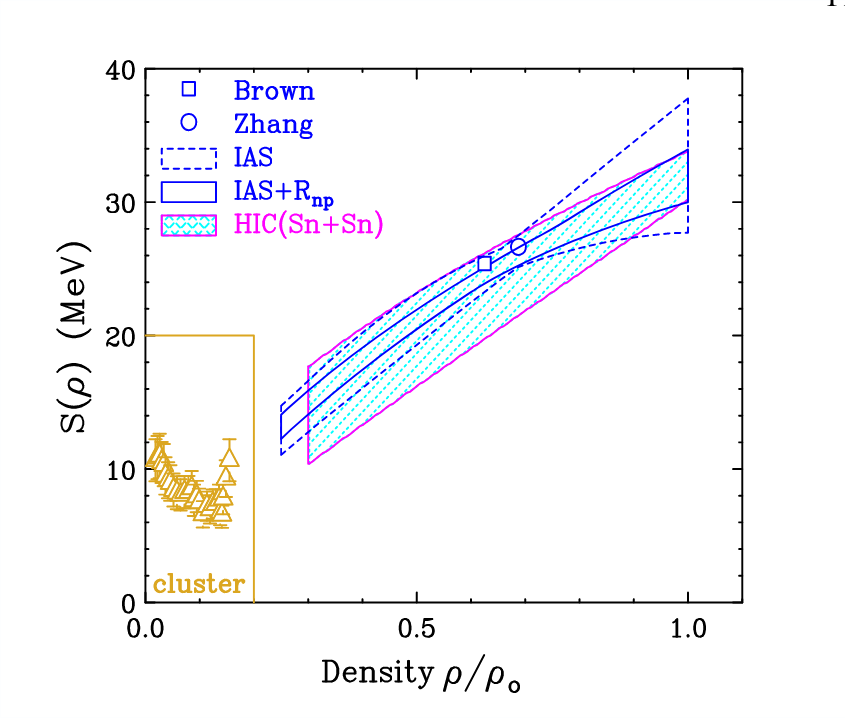
\includegraphics[scale=.5]{constraints}
\caption{Experimental constraints of the density dependence of the symmetry energy taken from \cite{awayforward}}
\label{fig:symDen}
\end{figure}


\section{Pion Observable}
It is preferable to find an observable that is easier to measure experimentally than neutrons, and is more sensitive to the high density region. Pions are produced though and intermediate process where nucleon-nucleon collisions form an excited $\Delta$(1232) baryon resonance from one of the nucleons, which then decay decay shortly after into a pion:

\begin{equation}
\ce{ NN <=> \Delta N <=> \pi NN}.
\end{equation}

The threshold for $\Delta$ resonance production, with a mass of \SI{1232}{\mega\electronvolt\per\clight\squared}, corresponds to a laboratory beam of \SI{290}{\MeVA} kinetic energy. In large nuclei the nucleons exist in orbitals which have large amounts of energy (Fermi energy), allowing for $\Delta$ production even at sub-threshold beam energies \cite{fermiEnergy}.


It has been shown in \cite{mingzhang} that most of the $\Delta$'s are produced in the early dense regions of the collision. Figure~\ref{fig:deltaProduction} shows the average local density (c) which $\Delta$'s are produced and the number in the system (b), as a function of time in the simulation of Au + Au collisions at \SI{400}{\MeVA}. Panel (a) shows the density distribution of the density at the moment of creation for $\Delta$'s. Since the average lifetime of the $\Delta$  is $\tau_{\Delta} = \SI{1.7}{\femto\metre\per\clight}$, the $\Delta$ resonance has very little time to be affected by the medium before decaying into a $\pi$ and nucleon. Thus the outgoing $\pi$ is contains information on the high density region of the collision. 

\begin{figure}[!htb]
\centering
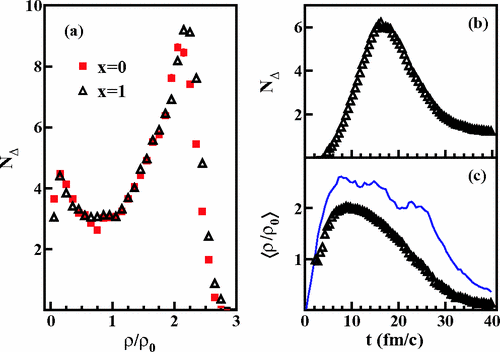
\includegraphics[width=.6\textwidth]{deltaProduction.png}
\caption{Figure taken from \cite{mingzhang} for Au + Au collisions at \SI{400}{\MeVA}. Panel (a) shows the density in the region of the $\Delta$ resonance creation for two different symmetry energies (x=0 soft) and (x=1 stiff). Panel (b) and (c) show the evolution of collision in time steps, where (b) shows the number of deltas in the system as a function of time and (c) shows the mean local baryon density in the region where $\Delta$ resonances are produced. The blue line in (c) represents the average baryon density in the most central region of the collision. This evidence shows that a majority of $\Delta$'s are produced in the high density region of the early collision.}
\label{fig:deltaProduction}
\end{figure}

The branching ratio of the various flavors of $\Delta$'s is given by the Clebsh-Gordon coefficients as shown in \ref{appen:deltadecay}. Here we see that in general proton-proton collisions give rise primarily to  $\pi^+$ and neutron-neutron collisions give rise to primarily $\pi^-$. In this $\Delta$ resonance model the charged pion ratio can be described as,

\begin{equation}
\frac{\pi^-}{\pi^+} = \frac{ 5pp + pn }{5nn + pn}.
\label{eq:deltaModel}
\end{equation}

In this $\Delta$ resonance model, $\pi^-/\pi^+ \approx (N/Z)^2$ where $N/Z$ is the neutron-proton ratio of the dense central collision where they are produced. Pions can be reabsorbed into a $\Delta$ resonance after colliding with the another nucleon in the froward and backwards process $\Delta <=> \pi + N$. This process generally dilutes the pion sensitivity to the high density region, since with each absorption and re-emission would change the pion dynamics or even the charge of the pion which would reflect the asymmetry at the point of creation and eventual re-emission. Total pion absorption back into two nucleons requires a three body process where a pion is absorbed creating a $\Delta$ resonance, then another nucleon must collide with the resonance to create two nucleons. Because of this, the total pion absorption (removing pions totally) is a less frequent effect than the absorption re-emission process. Yet in general by measuring the $\pi^-$ and $\pi^+$ is connected with n-n and p-p collisions. Instead of measuring neutrons we can measure the $\pi^-$ which is much easier to measure experimentally. 

\section{Motivation for Thesis}
In an effort to answer the high density behavior of the symmetry energy, we designed a new detector and a set of experiments of Sn + Sn collision utilizing inverse kinematics where the beam is made of a radio-active neutron rich beam. This allows for the neutron-proton asymmetry of the system to be changed depending on the beam. Pion production has been studied in stable beams for beam energies of \SI{400}{\MeVA} and above CITE HERE. Here only total pion yields were published and no pion spectra were published. The goals of this Thesis were to measure the pion spectra efficiently, to low pion energies. To do this a new Time Projection Chamber (TPC) was made, where we measured pions and light charged particles (up to Li) in neutron-rich heavy ion collisions at \SI{270}{\MeVA} 


%nuclear chart
%Dense nuclear matter 
%Liquid drop model explain density around saturation
%explain symmetry energy 
%extend to systems of larger pressure, isospin assymetry 
%symmetry energy how to calculate 
%Previous constraints on symmetry energy
%heavy ion collisions only way to probe density and 
%dynamics of proton neutrons 

%pion production 



\begin{comment}

\section{From Nuclear Forces to the Equation of State}
Isospin as a good quantum number at low energies 
Figure showing the nuclear forces for the pp, pn, nn 
Pauli exclusion 
inter particle distance , saturation density (maybe figure of all densities?)
Building the infinite matter
Statistical model 
Forces manifest in Energy/particle 

\section{The Nuclear Equation of State}
Figure showing the binding energy vs p-n asym
Liquid drop model, mass equation, move to higher densities
Symmetric EoS asymmetric EoS(symmetry energy)
Density dependence of the symmetry energy 

\section{Phases of Nuclear Matter}
gas liquid phase, gas, where are we
Progression through the heavy ion collision 
liquid, liquid gas, gas 

\section{Studying EoS through Heavy Ion Collisions}
going from infinite matter to finite matter 
approximate nuclear matter with neutron rich radioactive ion beams
probe different asymmetries 
probe different densities with different beam energies 
Symmetry energy goes down at higher beam energies

\section{Boltzmann Ulong Uhlenbeck (BUU) Transport Code}
Does not reach equilibrium for all observable (hadrons) what about pions?
Build up a mean field picture (momentum dependent) unknown quantities here
Non equilibrium can be solved with Boltzman equation with collision term and solved by MC
Figure of transport simulation code showing collision progression 
Clustering is an issue 
Meson, resonance production 

\section{Observables of interest to the EoS}
Particle yields of isospin opposites 
Flow??
Figure showing p-n observable lessens at high energy and from all densities 

\section{Pion Production }
Figure showing delta resonance 
Figure showing pion's produced at 2po 
Figure showing fermi motion effect (not really sub threshold but ok)
(chemical potential model, delta isobar) prediction for pion ratio
pion mass is small momentum shifted by coulomb affecting shape of pion spectra

\section{Previous Constraints}
Figure showing GW constraint and other previous constraints 
FOPI data at 400 A MeV not as sensitive to symmetry energy 
Saturation density and lower constrained but issues at high density
conflicting analysis on FOPI data which was not intended to be used for Symm Energy
Can you group all the constraints to one nice plot???

\section{Motivation for building the S$\pi$RIT TPC}
Based on EOS TPC
High efficiency for detecting pions and other light charged particles 
Effort to reduce the experimental error bars on such spectra which theory could use


\end{comment}
\chapter{Theory}
\section{From Nuclear Forces to Equation of State}
\section{Nuclear Equation of State}
\section{Boltzmann Ulong Uhlenbeck (BUU) Transport Code}
\section{Observables}
\section{The $\pi$ observable}
\chapter{Experiment}

\section{Operational Principles of Time Projection Chambers}

%explain in breif the basics of a time projection chamber 
\begin{figure}[!htb]
\centering
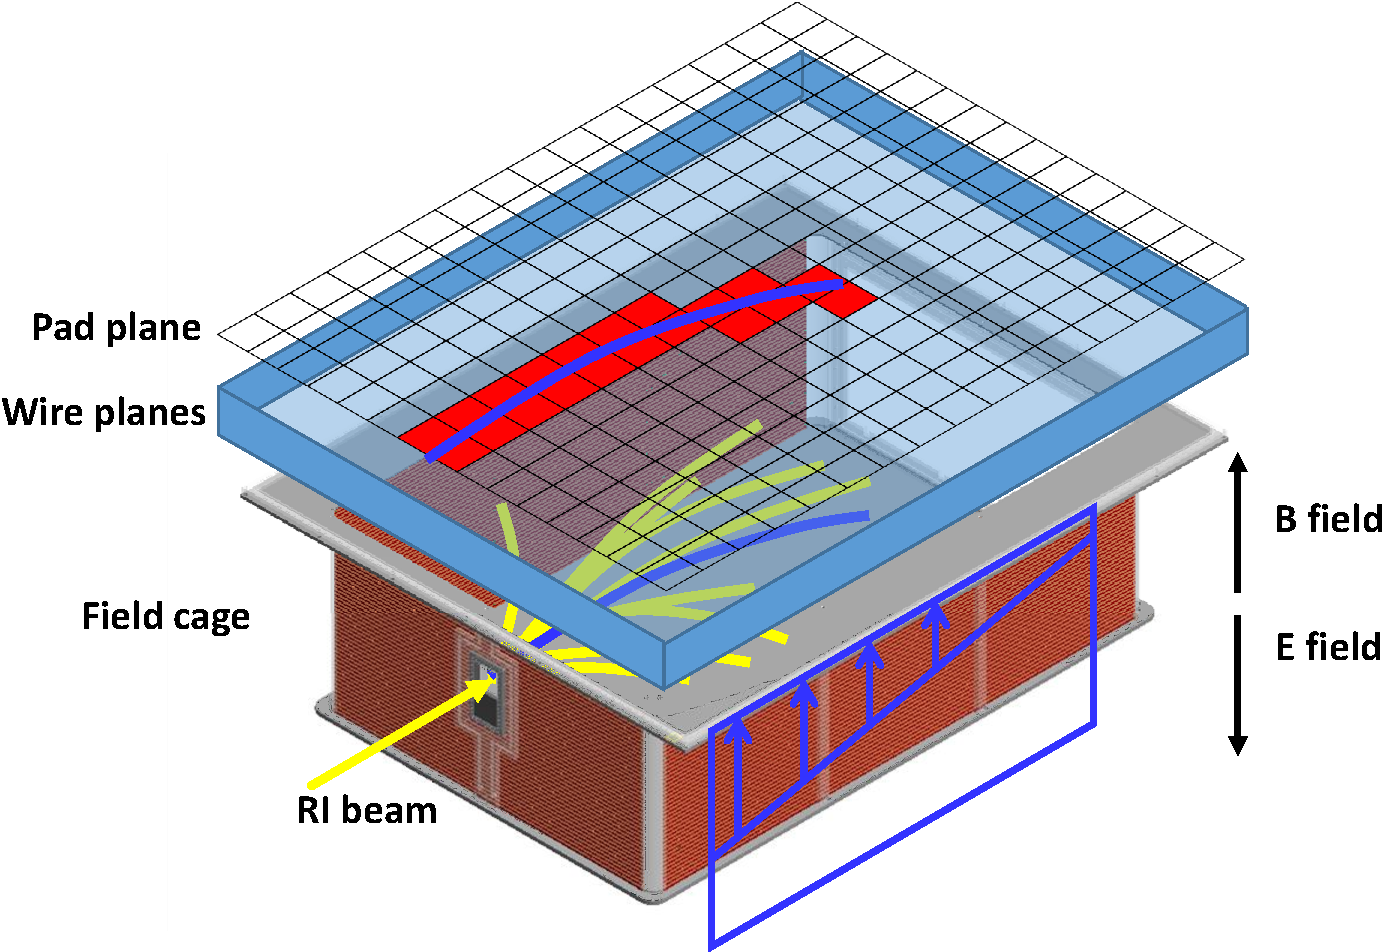
\includegraphics[scale=.5]{tpcPrinciple.pdf}
\caption{Operation principle of the TPC}
\label{fig:tpcPrinciple}
\end{figure}

%explain in breif the basics of a time projection chamber 
A Time Projection Chamber (TPC) is a detector that reconstructs the energy loss of charged particles and the location of that energy loss as in all 3 dimensions within the detector. TPCs have been employed in gases, liquid, and even solid detectors CITE HERE. In the following, we outline the physical principles involved in measurements within a gaseous TPC, and discuss the particular details of the TPC used in this thesis. Figure~\ref{fig:tpcPrinciple} depicts the interior of a gaseous TPC and its field cage. The field cage holds the detector gas and also defines a constant electric field that is typically aligned with the magnetic field of a magnet that surrounds the TPC. In this Spirit TPC, both these electric and magnetic fields are vertical.  

As a charged particle resulting from a heavy ion collision passes through the field cage, energetic \emph{primary} electrons are knocked out of neutral gas molecules and atoms in the detector gas. These primary electrons further ionize the detector gas until there is a distribution of \emph{secondary} electrons and positive ions that lie along the track's path. The electric field of the field cage separates these electrons and ions, where the electrons are accelerated upward by the electric field in the direction against the electric field, and the positive ions are accelerated along the electric field. Since the mean free path of the electrons inside the gas is very small, they quickly collide with other gas molecules, which slow down, or even stop the electron; only to be re-accelerated by the electric field, continuing a repeating cycle of stop and go motion. This microscopic behavior results in a constant drift velocity when averaged over multiple gas collisions. 

The electrons drift with this drift velocity through a set of wire planes, eventually reaching a set of high voltage anode wires, where they quickly accelerate in the presence of the high electric field emanating from the anode wires. This high electric field imparts enough energy between collisions to ionize the gas, creating additional electron-ion pairs from the gas, culminating in an avalanche process near the anode wires. The avalanche electrons typically terminate on the anode wire,  while the ions created in the avalanche are accelerated  away from the anode wires. This ionic motion induces image charges in nearby pads within the pad plane that is located close to the anode wires. The corresponding image currents in these pads are read out by electronics that are attached to these pads. This electronics signal encodes the energy loss information and arrival time of the signal from the electrons drifting from the ion track, and can be analyzed to determine the position of the ion track within the TPC. 

The pad plane is perpendicular to the electric field of the field cage and is divided into a two dimensional grid of pads. Two of the 3 coordinates are determined from the 2-dimensional charge distribution corresponding to the projection of the track onto the pad-plane. The third dimension comes from extrapolating the electrons back in time, utilizing the known constant drift velocity $v_d$. The distance the electron has traveled , $d$, -- along the electric field direction-- is calculated as $d = v_d \cdot t$, where $t$ is the drift time information obtained from combining the time of the event trigger with arrival time of the signal from the  electrons in the electronics. The radius of curvature of the track on the pad plane is related to the magnetic rigidity, and therefore the momentum of each track. The energy loss deposited $\langle dE/dx\rangle$ is proportional to the image charge induced on the pads on the pad-plane. With these two observations, particles can be uniquely identified by their mass and charge since there is a unique correlation between the rigidity and $\langle dE/dx\rangle$  lines. This correlation allows the particle type to be identified as discussed later in Section~\ref{sec:pid}. In this chapter we will provide more details about the particle detection within the \spirit TPC  that is relevant to the reactions studied in this thesis. 


\section{S$\pi$RIT TPC Overview}
%Add Overview image with labels

\begin{figure}[!htb]
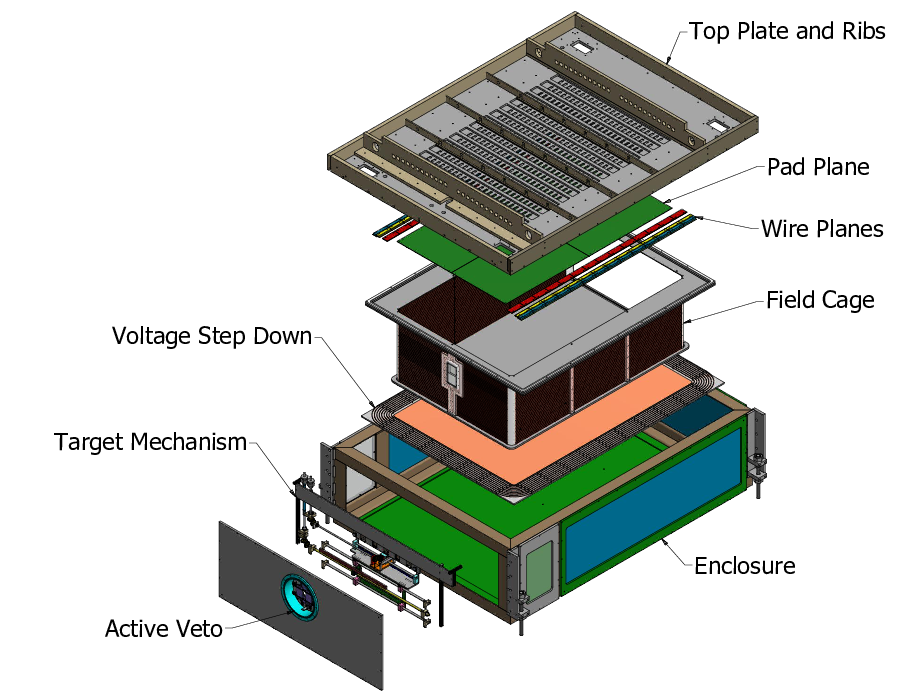
\includegraphics[width=\textwidth]{exploded.png}
\caption{Overview of the \spirit TPC}
\label{fig:tpcExplode}
\end{figure}


The Samurai Pion-Reconstruction and Ion Tracker Time Projection Chamber (\spirit TPC) was developed to measure pions and other light charge particles produced in collisions of radioactive rare isotope beams with stable targets in fixed target experiments.  The TPC is built on an aluminum angle iron skeleton with thin aluminum sheet walls in order to minimize neutron scattering and to allow for light charged particles to reach auxilliary detectors on the sides and downstream of the TPC. The \spirit TPC was developed to fit inside the SAMURAI dipole magnet used at the Rare Isotope Beam Factory (RIBF) at RIKEN in Wako-shi, Japan \cite{riken}. The dipole gap limited the vertical space of the TPC to around \SI{75}{\centi\metre}. More detail and specifications of the SAMURAI dipole magnet are given in \cite{samurai}. 

The exploded drawing shown in Fig.~\ref{fig:tpcExplode} illustrates these major internal components of the  of the \spirit TPC. A target mechanism allowed for up to 5 fixed targets to be mounted on the target ladder situated just upstream of the field cage, where changing the targets could be performed outside of the magnet. Reaction products from nuclear collisions exit the target and enter the field cage of the TPC. The field cage contains the detector gas and defines the constant electric field. It is rigidly mounted to the large aluminum top plate of the TPC gas containent vessel. The field cage is electrically isolated from the top plate by a lexan top perimeter ring with o-rings to provide as gas seal. The pad plane and wire plane structures are  mounted to the inside face of the top plate with the electronics being mounted on the outside face of the top plate. Several aluminum ribs were also mounted to provide extra rigidity to the top plate, keeping it flat to within \SI{150}{\micro\metre}, as measured by a precise laser measurement \cite{jon}. Holes in the top plate allowed signals from the individual charge sensitive pads on the pad plane to be transmitted via cables to the electronics. 



\begin{table*}\centering
\ra{1.3}
\begin{tabular}{@{}rr@{}}\toprule 
\multicolumn{2}{c}{\spirit TPC Overview} \\
 \midrule
Pad plane area & 1.3 m x .9 m\\
Pad size       & 1.2 cm x .8 cm \\
Number of pads & 12096 (112 x 108) \\
Gas composition& 90\% Ar + 10\% CH${}_4$ (1 atm)  \\
Multiplicity limit & 200  \\
dE/dx range        & Z=1-3, $\pi$, p, d, t, He, Li \\
Drift length       & 50 cm \\
\bottomrule
\end{tabular}
\caption{An overview of the properties of the \spirit TPC}
\label{tb:spiritoverview}
\end{table*}


\begin{comment}
\subsection{Enclosure}
The skeleton of the enclosure is composed of a rigid rectangular aluminum angle-iron frame. To this frame, six rectangular sides are attached. The downstream window and the two side windows are constructed of a aluminum window frames with a 1 mm  aluminum sheet metal window. These thin sheet metal windows allow charged particles and neutrons to exit the TPC without significant energy loss or scattering. This allows for a trigger to be created by placing detectors outside of  the side windows and downstream window of the TPC. The enclosure itself is made to be gas tight with no leakage from the outside or from the interior of the field cage. This is to allow for the possibility to choosing one insulation gas outside of the field cage and a different counter gas inside the field cage. In the first campaign of experiments, however, we used the same gas in the field cage and enclosure volume.  
\end{comment}

\subsection{Field Cage}
%The field cage contains the detector gas and defines a uniform electric field in which electrons can drift upwards toward the anode wires. It was designed to hang from the top plate and therefore needed to be of a lightweight construction and the materials needed to be thin to allow for light charged particle and neutrons to pass through to ancillary trigger detectors without significant energy loss or scattering .  

\begin{figure}[!htb]
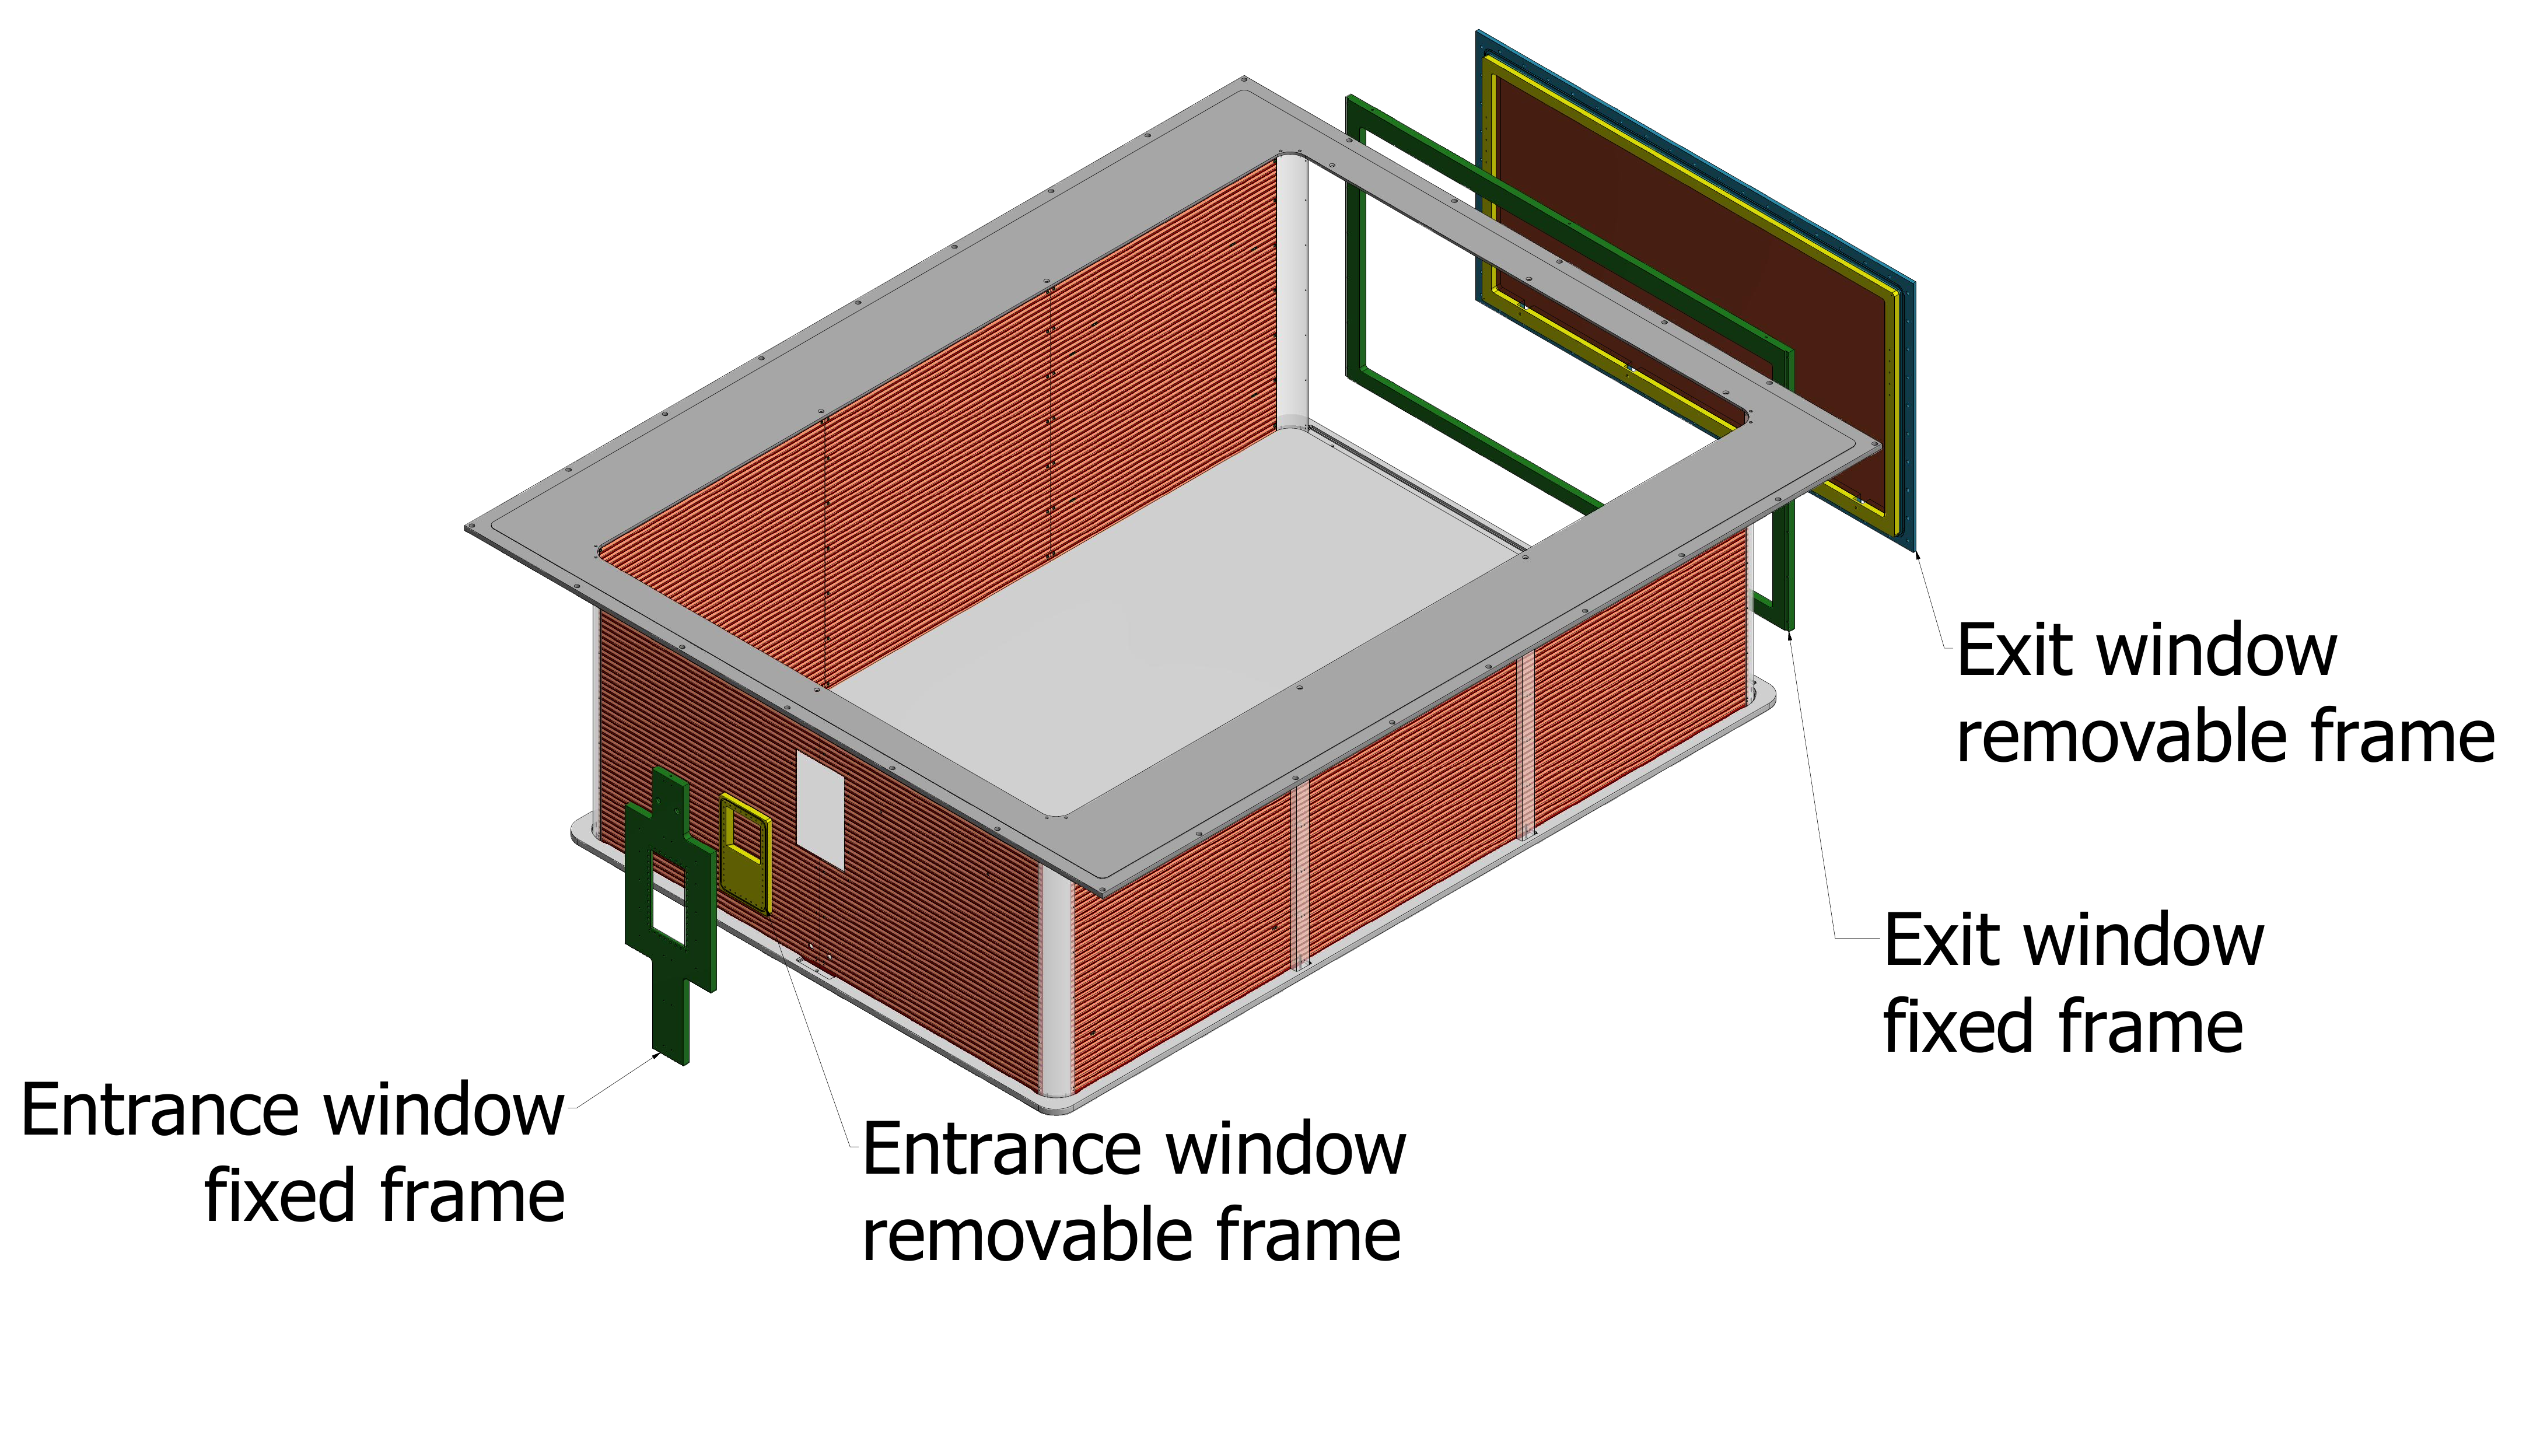
\includegraphics[width=\textwidth]{fc_overview.png}
\label{fig:fc_overview}
\caption{FC overview}
\end{figure}


\begin{figure}[!htb]
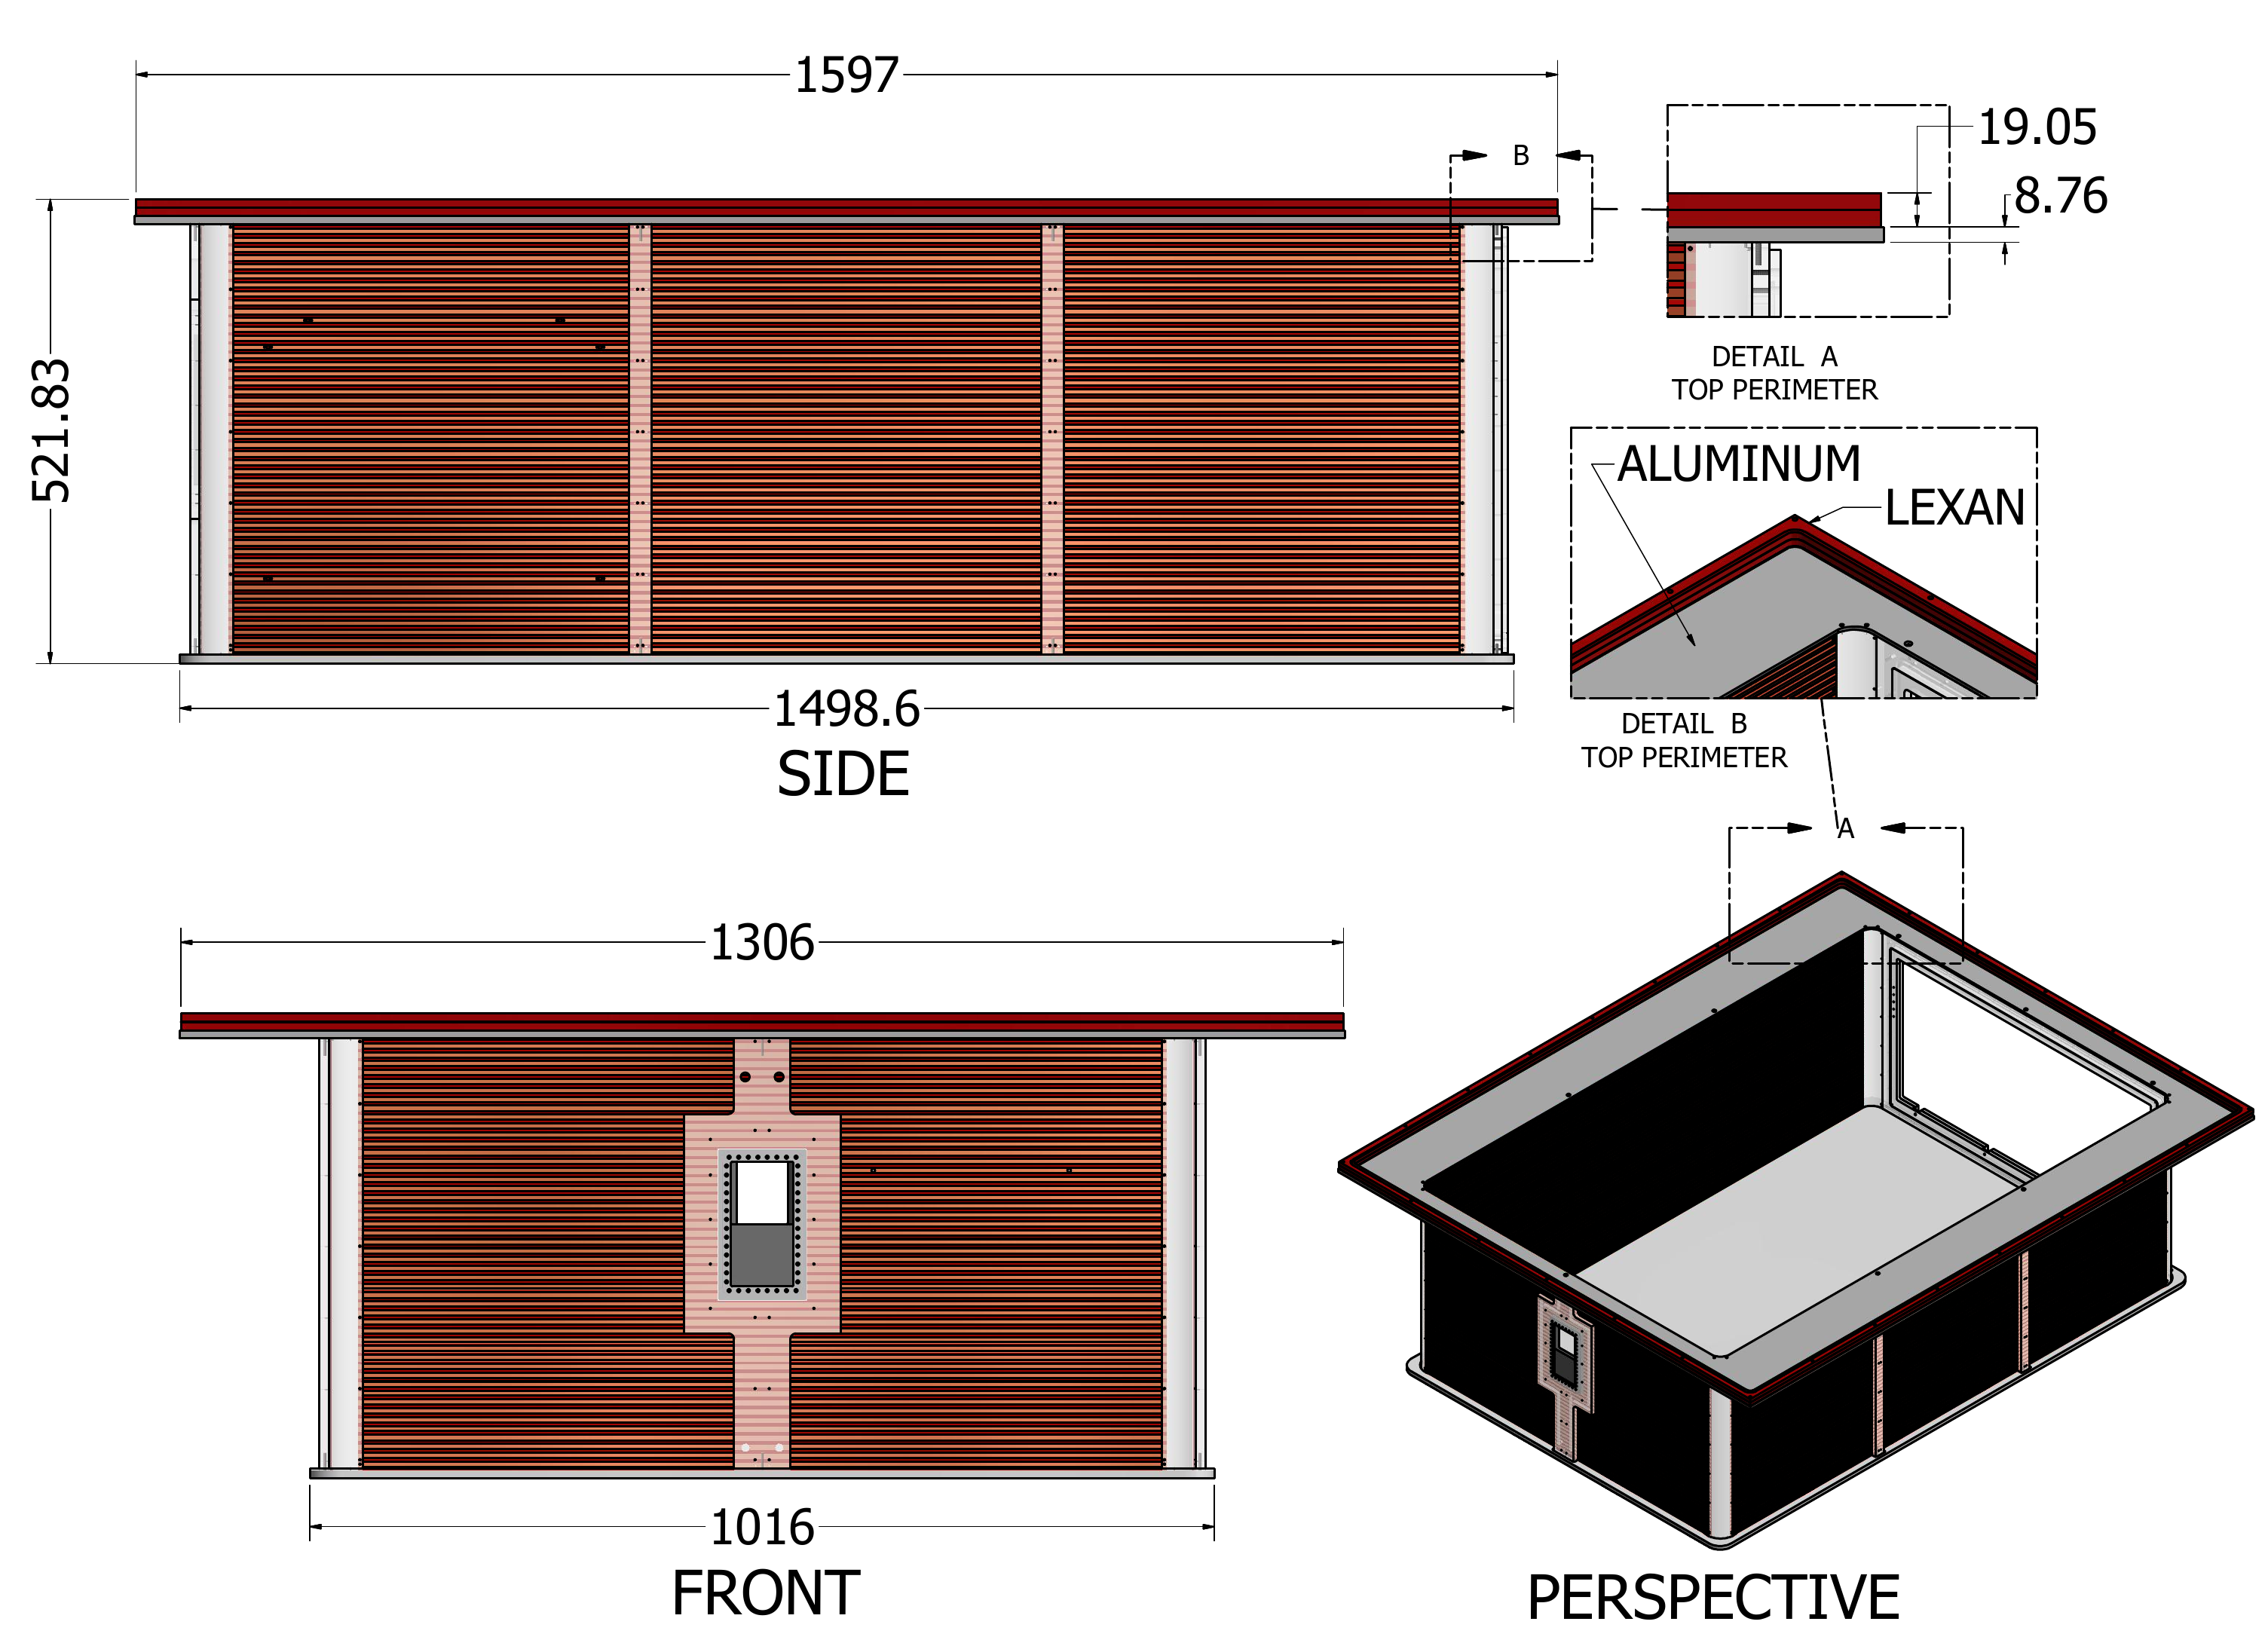
\includegraphics[width=\textwidth]{fc_overview2.png}
\label{fig:fc_overview2}
\caption{FC overview 2}
\end{figure}


The field cage was constructed from several panels of two-layer printed circuit board (PCBs). The front of the field cage was made of two PCBs and each side was constructed from three PCBs. These boards had copper strips etched onto the inside and outside of the board which when all the boards were assembed, formed copper rings which were used to set up the uniform electric field, as will be described later. The array of circuit boards were glued and supported by Lexan pieces. We did not use the common PCB substrate material FR4, which contains a Bromine impregnated epoxy which can outgas Bromine, which can absorb the secondary electrons from the track, thereby degrading the signal \cite{tpcAging}. Instead, a halogen free material, Cryogenic-G10, was used for the board material.  The downstream wall mainly consists of a large, thin exit window. The window  is constructed of   \SI{10}{\micro\metre} Kapton upon which are  evaporated aluminum strips that define the electric field. At the bottom of field cage is the cathode that is  constructed from an aluminum honeycomb laminate, composed of two aluminum sheets bonded to an aluminum honeycomb core, providing a lightweight yet rigid structure. On the other end the boards were epoxied into an aluminum top perimeter which also served as the last electrode ring in the TPC. Together with the cathode bottom, the field cage proved to be a rigid lightweight structure. A Lexan ring containing o-rings was placed in-between the top perimeter piece and the top plate of the TPC. Screws with nylon washers, and collars, were used to mount the top perimeter, and the field cage, to the top plate; it also provided electrical isolation from the top plate. In this way the top plate could be removed and rotated with the field cage attached, without damaging any internal components. 

\begin{figure}[!htb]
\centering
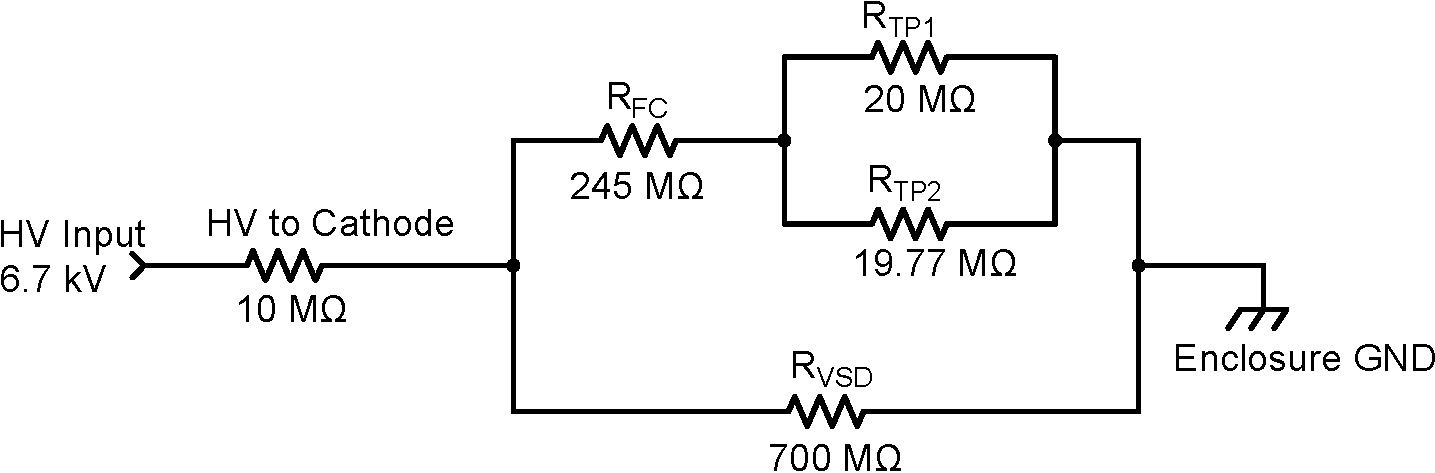
\includegraphics[width=\textwidth]{TPC_schematic.pdf}
\caption{Schematic of the TPC system}
\label{fig:TPC_schematic}
\end{figure}



Figure~\ref{TPC_schematic} shows the schematic of the effective resistances and capacitance of the TPC subsystem. The cathode is connected to the high voltage (HV) supply through a \SI{10}{\mega\ohm} resistor and has an effective capacitance to ground of \SI{4}{\nano\farad}, $C_{VSD}$. The cathode voltage $V_{cath}$ can be calculated as,
\begin{equation}
V_{cath} = \frac{V_{HV}}{ 1 + \frac{10}{ \left( (245 + R_p)^{-1} + 700^{-1} \right)^{-1} } },
\end{equation}
where 
\begin{equation}
R_p = \left( R_{TP1}^{-1} + R_{TP2}^{-1} \right)^{-1},
 \label{eq:Reff}
\end{equation} 

is the effective resistance of the last resistor, and $V_{HV}$ is the high voltage supply; all resistor values are given in \si{\mega\ohm}.


\begin{figure}[!htb]
\centering
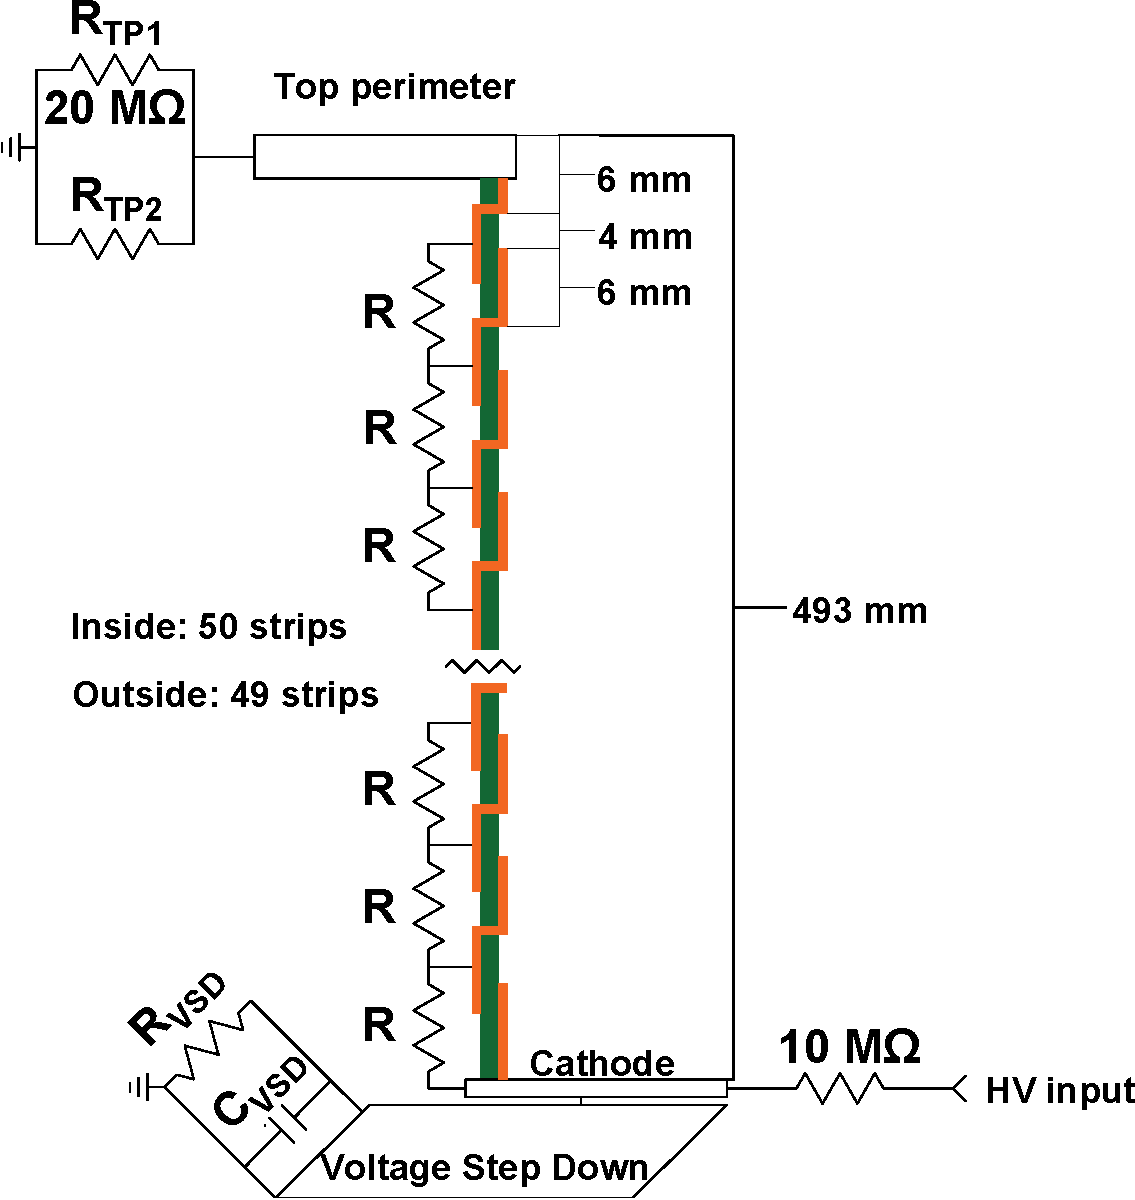
\includegraphics[scale=.6]{FC_schematic.pdf}
\caption{Schematic of the electric connections relevant to the Field Cage system. The strip thickness is exaggerated in the figure to show the detail}
\label{fig:FC_schematic}
\end{figure}

Figure~\ref{fig:FC_schematic} shows a schematic detailing the connections involved in the field cage walls. The field cage contains 50 inside copper strips and 49 outside copper strips. The strips are \SI{6}{\milli\metre} in width and spaced \SI{10}{\milli\metre} apart. Since the field cage was build with an array of PCB boards, connections from adjacent strips were connected all the way around until all the strips formed a continuous ring. The interfaces were the side pieces met were connected by G-10 corner pieces where conductive paint strips were painted on. The first inside strip is connected to the cathode, which is itself connected by an effective \SI{5}{\mega\ohm} resistor ($R$) to the first outside strip. The first outside strip is connected through a via to the second inside strip. These outside strips formed a small electric field which repelled electrons away from the PCB substrate between inside strips, preventing build up on the insulating material. This pattern repeats until the very last strip. A resistor chain, connected to the outside strips, creates a voltage divider in which each strip is separated by a constant difference voltage and a fixed distance, setting up a constant electric field. The last strip of the field cage is composed of a small inner strip  (\SI{1.5}{\milli\metre}) on the PCB board and the top perimeter piece (\SI{4.5}{\milli\metre}) giving an  effective thickness of \SI{6}{\milli\metre}, which is the same as the other strip widths. The top perimeter is connected to electrical ground through a \SI{20}{\mega\ohm} resistor ($R_{TP1}$) with the option to place an additional resistor ($R_{TP2}$) in parallel to tune the voltage of the top perimeter, as seen in Fig.~\ref{fig:FC_schematic}. Allowing for a tunable resistor allowed for fine tuning of the electric field in the region between the top perimeter and the wire planes as will be discussed in Section~\ref{sec:wireplanes}. 

The voltage on each strip, $V_n$, can be expressed as, 
\begin{equation}
V_n = V_{cath} \frac{R_p + (50 - n)R}{49\cdot R + R_p}
\label{eq:FCstrip}
\end{equation}

where $n = 1$ represents the index of the first inside strip, and $n= 50$ represents the index of the last inside strip, which is the same as the top perimeter voltage.



%Talk about the uniforminty of the field cage maybe
%how far the wall was from the pad plane on the sides talk about the front


\subsection{Voltage Step Down}
The gap between the cathode and the ground of the enclosure is quite small. To prevent electric breakdown in the gas between this gap, a series of concentric copper rings safely stepped down the voltage to ground in a controlled manner, reducing the chance of electric breakdown and sparking. There were 8 concentric rings with a \SI{10}{\mega\ohm} resistors in between, creating a resistor chain which steps down the voltage each ring by approximately \SI{1000}{\volt} each time. The first ring is the same voltage as the cathode and the last ring is connected to ground. All together the total resistance of the resistor chain is \SI{700}{\mega\ohm}.


\subsection{Wire Planes}
\label{sec:wireplanes}
%Add figure of gating grid transparency closed and open configuration 

There are three wire planes that are mounted underneath the pad-plane. The wire plane closest to the pad-plane (\SI{4}{\milli\metre}) are the anode wires. The next plane (\SI{8}{\milli\metre}) is the ground plane or Frisch grid. The last plane (\SI{14}{\milli\metre}) is the gating grid. The gating grid is the first plane that electrons meet as they drift upward from the field cage volume towards the anode plane. The gating grid functions as a gate, either allowing electrons and ions through, or blocking them entirely. The ground plane functions to shield the inside volume of the TPC from the high electric field surrounding the anode wires. The ground plane is the least interesting plane and is held to ground by shorting the plane to the enclosure ground through shorted BNC terminator on the outside of the TPC. We also use the ground plane to input a pulser, which is used to spread the pulsed signal to all the pads on the TPC in order to calibrate the electronics of the TPC. This is done by replacing the shorted BNC with a \SI{50}{\ohm} termination and injecting the pulser on the other end. 


 \begin{table*}[!htb]
 \centering
\ra{1.3}
\begin{tabular}{@{}rrrrrrr@{}}\toprule 
\multicolumn{2}{c}{GET electronics settings}\\
\midrule
 Plane & Material & Diameter \si{\micro\metre} & Pitch \si{\milli\metre} & Distance to pad-plane & Tension \si{\newton} & Voltage \si{\volt}\\ [0.5ex] 
 Anode  & Au-plated W   &  20  &  4  &  4   &  0.5  &  1460  \\
 Ground & BeCu          &  75  &  1  &  8   &  1.2  &  0     \\ 
 Gating & BeCu          &  75  &  1  &  14   &  1.2 &  -110$\pm$ 70\\ 
 \bottomrule
\end{tabular}
\caption{Wire plane properties}
\label{tb:wireplane}
\end{table*}

In the open configuration, the gating grid is transparent to electrons coming from the field cage volume and also allows for ions to move from the avalanche region into the TPC volume. In the closed configuration it is opaque to electrons and ions, when set to the right voltages. Typically the gating grid is always in the closed configuration, only opening it momentarily when the data acquisition trigger criteria is met to take data. By keeping it always closed the electrons which come from the un-reacted beam are blocked,  which if allowed to go to the anode wires, would quickly build up enormous amounts of positive ions, which would flood the field cage with space charge, distorting the electrons represnting the track paths. We open the gating grid for about \SI{11}{\micro\second} which is more than the time it takes for the electrons to drift one TPC volume. After this, we close the gating grid to prevent the back-flow of ions from the avalanche region from that event. Since ions move with a velocity much slower than that of electrons \cite{blumrol}, the ions only move several \si{\micro\metre} in the time the gate is open. This allows for electrons to pass through while preventing the back-flow of ions into the FC volume, reducing or even eliminating the space charge resulting from the avalanche region.

Figure~\ref{fig:gg_onoff} shows a Garfield simulation of the drift lines of electrons in both the on and off configurations. In the on configuration, all the wires share the same average voltage, $V_{g.g.}$, which is set to the optimal voltage that represents of 100\% electron transparency. Figure~\ref{fig:wires_open} shows the electrons are allowed to drift completely through the gating grid all the way to terminate on the anode wires. In the off configuration, the reference voltage $V_{g.g.}$ remains the same, but alternating wires get an offset voltage of $\pm \Delta V$, so that the electric field produced by the voltage difference $2\Delta V$ between wires is great enough to block incoming electrons. Figure~\ref{fig:wires_closed} shows this case were the electron drift lines are fully blocked, as they terminate on the more positive wires. Opening the grid from this closed bi-polar mode is simply done by removing the offset voltage and allowing the two wires to short which equilibrates their charges, coming back to the average voltage setting in the on configuration.

\begin{figure}[!htb]
    \centering
    \begin{subfigure}[t]{0.49\textwidth}
        \centering
        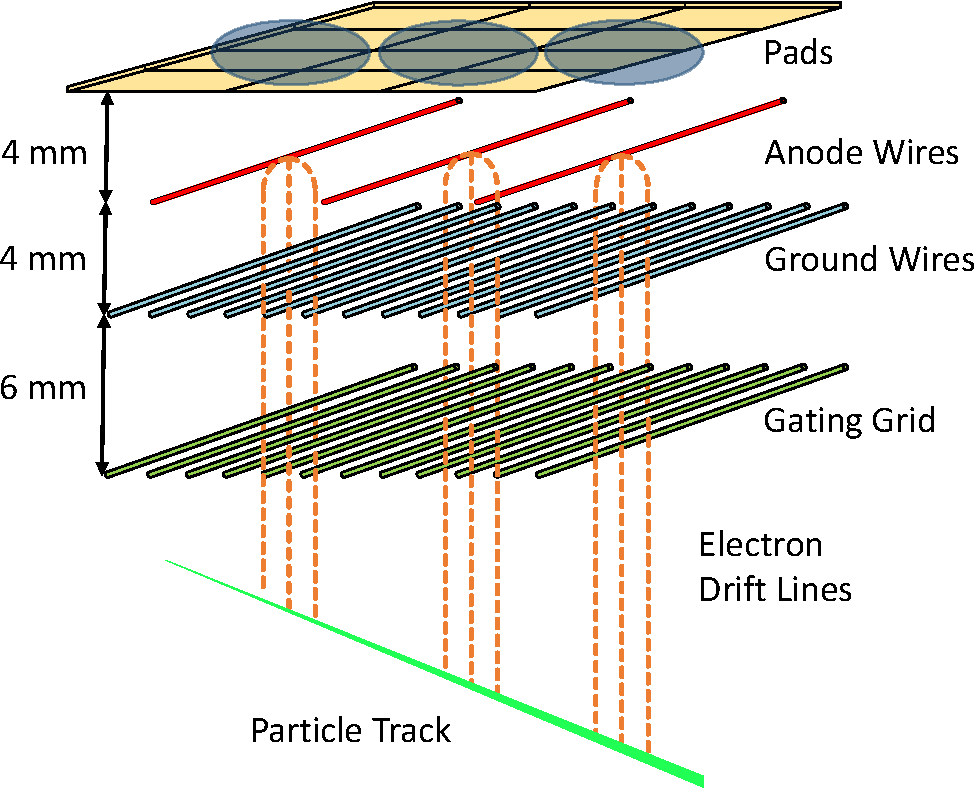
\includegraphics[width=\linewidth]{wires_open.pdf} 
        \caption{Wires open} \label{fig:wires_open}
    \end{subfigure}
    \hfill
    \begin{subfigure}[t]{0.42\textwidth}
        \centering
        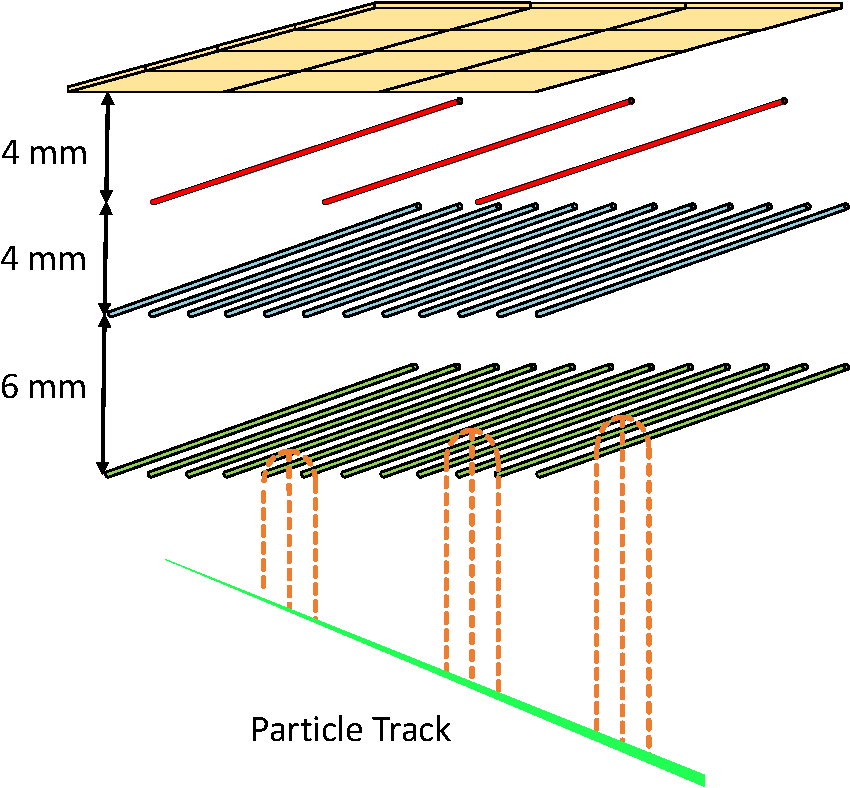
\includegraphics[width=\linewidth]{wires_closed.pdf} 
        \caption{Wires closed.} \label{fig:wires_closed}
    \end{subfigure}
\label{fig:wires}
\end{figure}



\begin{figure}[!htb]
\centering
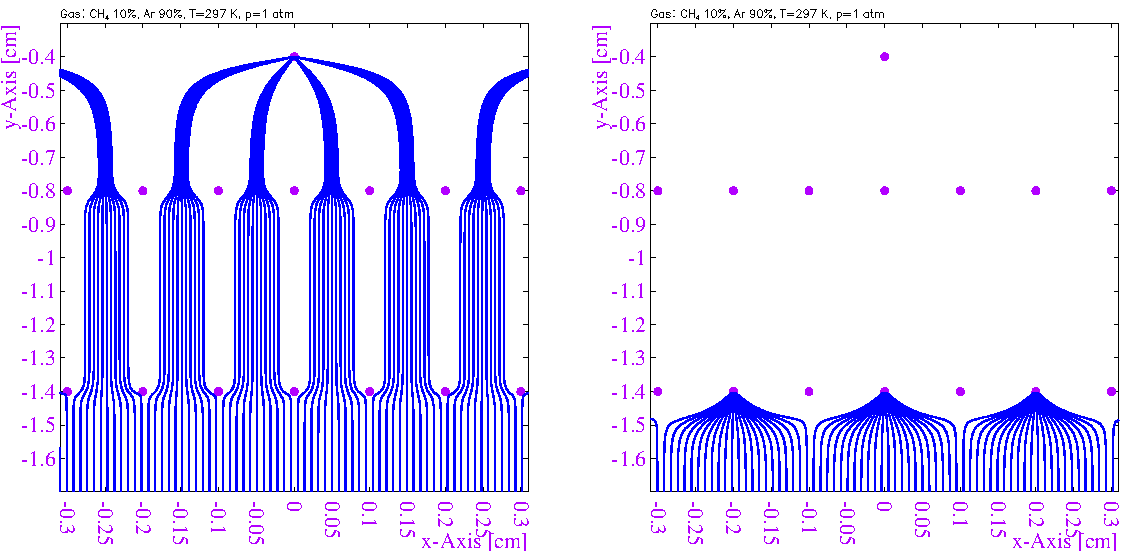
\includegraphics[width=\textwidth]{gg_onoff.pdf}
\caption{On and off configurations of the gating grid.}
\label{fig:gg_onoff}
\end{figure}


Both configurations of the gating grid were measured and simulated. To measure the electron transparency in the on configuration all wires were set to the same voltage $V_{avg}$, and the anode wires were lowered to \SI{500}{\volt}. By lowering the voltage of the anode wires we could measure the large charge of the beam without saturating the electronics. The average charge deposited in the chamber was measured as a function of $V_{avg}$. Changing the average voltage required a different top perimeter resistor value according to Eq.~\ref{eq:TP_resistor}. Several runs were taken ranging from \SIrange{-198}{-40}{\volt}, with and without the magnetic field. Theoretically the most negative value represents 100\% electron transparency and was used as the reference run in which we scaled all measurements to. The measured electron transparency, $T$, was estimated as $T = \langle dE/dx\rangle/{\langle dE/dx\rangle}_{ref}$, where $\langle dE/dx\rangle_{ref}$ represents the average energy loss of the reference run. Figure~\ref{fig:ggAvgTrans} shows the measured transparency as a function of $V_{avg}$, as compared with the corresponding Garfield simulation \cite{garfield++}. The average gating grid voltage used in the experiment was \SI{-171}{\volt} to ensure we were well within the 100\% transparency region. 

To measure the electron transparency as a function of the difference voltage $\Delta V$, the average voltage was first set to 100\% transparency, $V_{avg}=\SI{-171}{\volt}$, and the difference voltage was added and subtracted from alternating wires. Figure~\ref{fig:ggDeltaVTrans} shows the result of the simulation and experiment with and without the magnetic field. By introducing the magnetic field the required voltage to close the grid increased as expected. In the experiment we selected the value of $\Delta V = \SI{65}{\volt}$ to ensure we were well within the region of 0\% transparency. In both the on and off configurations good agreement was seen with the corresponding Garfield++ simulations when accounting for statistical error in the MC simulations and in the data.   

\begin{figure}[!htb]
    \centering
    \begin{subfigure}[t]{0.49\textwidth}
        \centering
        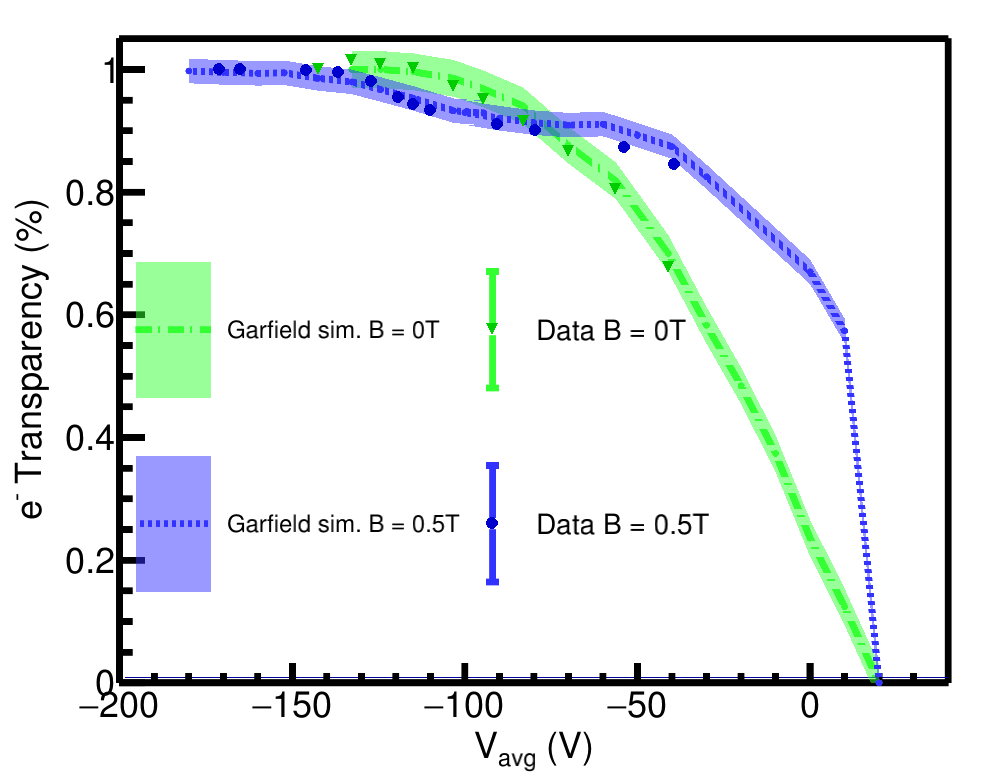
\includegraphics[width=\linewidth]{averageTransparency.png} 
        \caption{Electron transparency for the conditions of all wires are the same voltage.} \label{fig:ggAvgTrans}
    \end{subfigure}
    \hfill
    \begin{subfigure}[t]{0.49\textwidth}
        \centering
        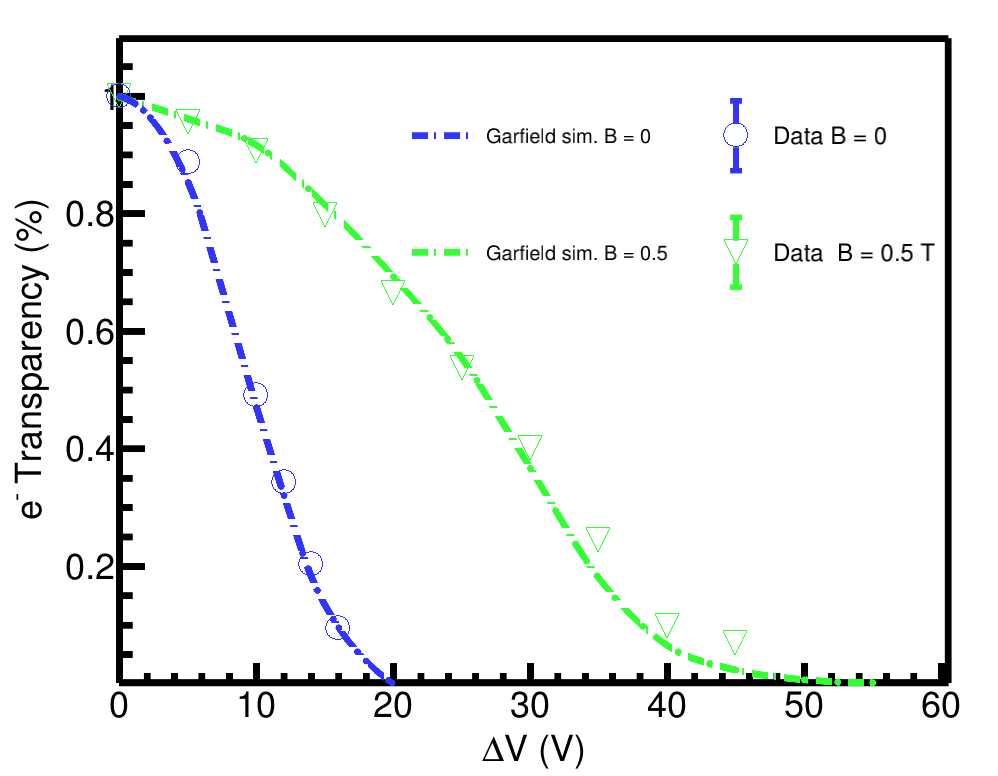
\includegraphics[width=\linewidth]{transparencyDeltaV.png} 
        \caption{Electrons transparency for the mode where adjacent wires have a voltage difference of $2 \Delta V$.} \label{fig:ggDeltaVTrans}
    \end{subfigure}
\label{fig:ggTrans}
\end{figure}



The anode wires are made of very thin Gold plated Tungsten wires, about \SI{20}{\micro\metre} in diameter. They are biased to high voltages of about  \SI{e3}{\volt} which creates a very high electric field very close to the anode wire. As the electron approaches the anode wire, the field gets strong enough that the kinetic energy gained between collisions exceeds the ionization potential of the gas nocking out more electron-ion pairs in the gas. This happens over several collisions creating an avalanche effect amplifying the electron current.  The final number of electrons produced depends on the anode wire voltage and the gas properties. The absolute gas gain was not experimentally determined but it was calculated in a Garfield simulation. For the experimental data pertaining to this disertation, the anode wires were biased to two different voltages. We will refer to the voltage \SI{1460}{\volt} as the \emph{high voltage} and \SI{1214}{\volt} as the \emph{low voltage}. Two sections were biased with the lower voltage setting to minimize the effects of a leakage of secondary electrons around the end of the gating grid \cite{jon}.


 Figure~\ref{fig:anodegain} shows the electron distribution for the total number of electrons produced in a avalanche process created by a single electron. The distribution follows the expected Polya distribution, and the MC data in the simulation was fitted with a Polya function \cite{blumrol}, which can be expressed as,

\begin{equation}
P(x) = A_0^{-1}\cdot \frac{A_1^{A_1}}{\Gamma(A_1)} \left(\frac{x}{A_0}\right)^{A_1-1}e^{\frac{-A_1x}{A_0}}.
\end{equation}

For the voltage of \SI{1460}{\volt} the parameters of the fit are $A_0=903.9$ and $A_1=1.50$ and for the voltage of \SI{1214}{\volt} the parameters are $A_0=150.0$ and $A_1=1.47$. These Polya distribution fits will be important later as the input to the Monte Carlo simulations of the detector response in Section~\ref{sec:monteCarlo}.



\begin{figure}[!htb]
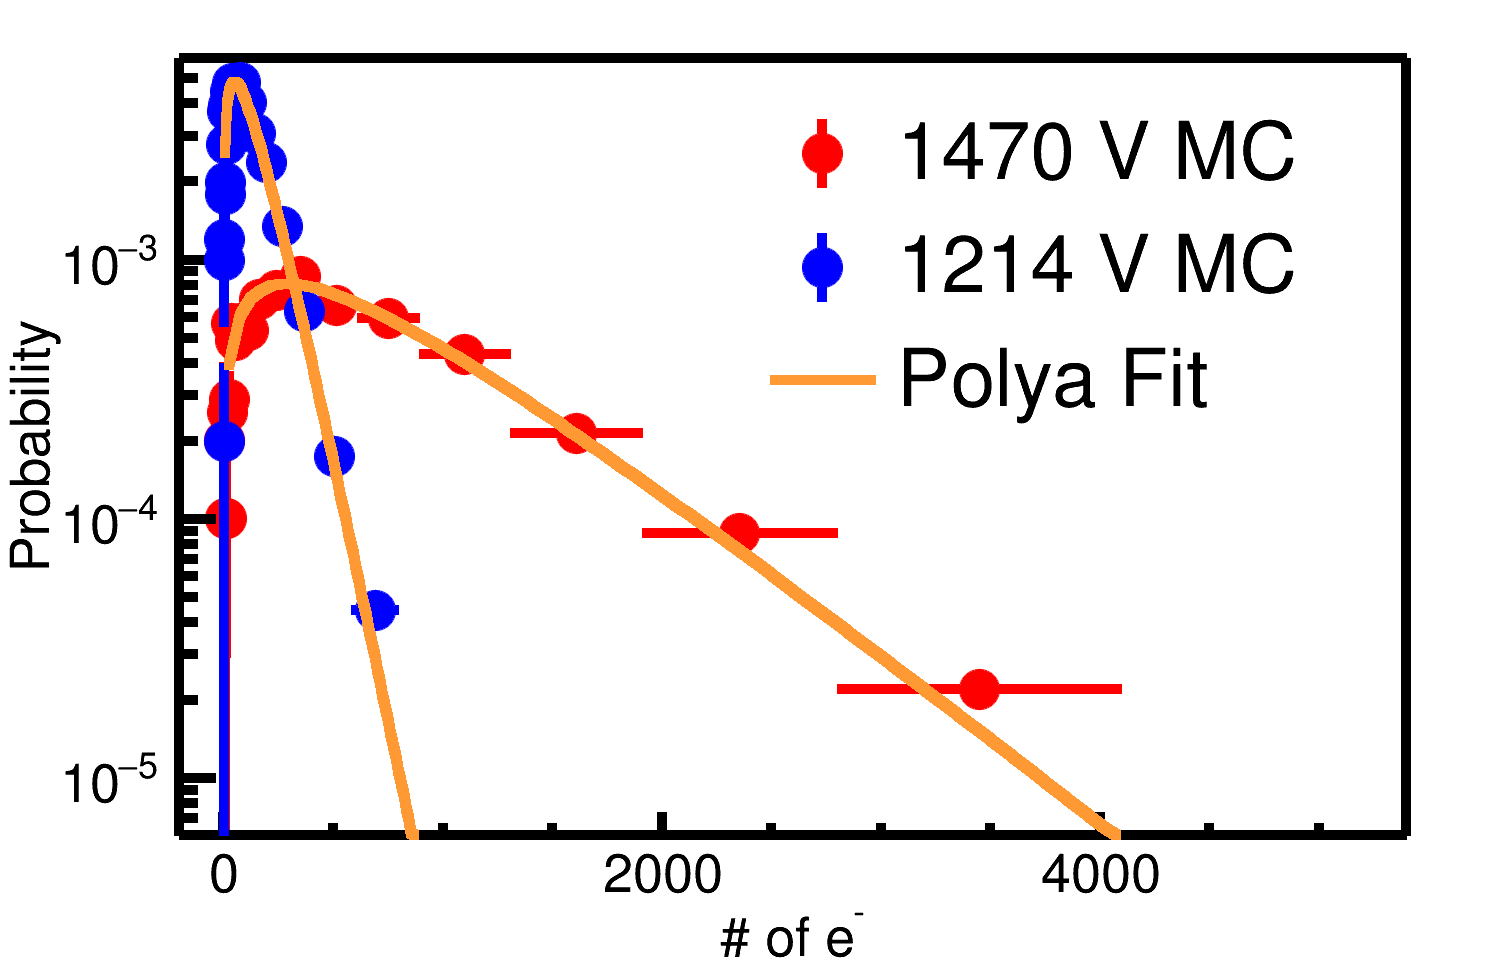
\includegraphics[width=\textwidth]{gain.png}
\caption{Number of electrons produced in a single avalanche on an anode wire. Two different voltages were simulated using Garfield++ at 1470 $V$ and 1214 $V$. The expected Polya distribution fit is also given in yellow.}
\label{fig:anodegain}
\end{figure}



Care must be taken to choose the resister ($R_{TP2}$) that connects the field cage divider chain to the top plate. The end of the field cage nearest to the top plate is at the same potential as the aluminum top perimeter piece to which the field cage is glued. This top perimeter piece forms a horizontal surface that is an equipotential representing the last ring. The voltage difference between the average voltage on  the gating grid and the voltage of the top perimeter influences the electric field just below the gating grid. If $R_{TP2}$ is incorrectly chosen, the electric field near the gating grid will be different for electrons that pass near the field cage walls than it is for electrons in the center of the TPC,  causing distortions of the tracks in the TPC. This requires the value for $R_{TP2}$ to be chosen correctly. Since this simple point can be easily forgotten, we now discuss this choice in greater detail.

To understand how to calculate $R_{TP2}$ we imagine the space between the cathode and the gating grid can be split into two virtual volumes, Region 1 defined as the space between the cathode and the top-perimeter, and Region 2 defined between the top-perimeter and the gating-grid. The magnitude of the electric field in the region between the top-perimeter and the cathode, $E_1$, is defined as,

\begin{equation}
E_1 = \frac{V_{g.g.} - V_{tp}}{ y_{g.g.} - y_{tp} },
\end{equation}
where  $V_{g.g.}$, $V_{tp}$ , $y_{g.g.}$, and $y_{tp}$ are the voltages and vertical y-positions of the gating-grid and top-perimeter respectively. The y-position here refers to the center of the electrodes. The magnitude of the electric field in the region between the top-perimeter and the cathode, $E_2$, is defined as,

\begin{equation}
E_2 = \frac{V_{tp} - V_{cath}}{ y_{tp} - y_{cath} },
\end{equation}
where  $V_{tp}$, $V_{cath}$ , $y_{tp}$, and $y_{cath}$ are the voltage and vertical y-position of the top-perimeter and cathode respectively. The y-position of the cathode is defined as the face of the cathode. The condition for a smooth electric field across these two virtual volumes is defined as the solution to the equation $E_1 = E_2$. Substituting Eq.~\ref{eq:FCstrip} for $V_{tp}$ -- $n=50$ -- we can solve for the effective resistance of the top perimeter $R_p$ as, 

\begin{equation}
R_p = 49 \cdot R  \left(\frac{ y_{g.g.} - y_{cath} }{ y_{TP} - y_{cath} \frac{V_{cath} - V_{gg}}{V_{cath}} }- 1 \right),
\label{eq:TP_resistor}
\end{equation}

where the relevant vertical dimensions are $y_{g.g.} - y_{cath} = \SI{497.3}{\milli\metre}$ and $y_{tp} - y_{cath} = \SI{490}{\milli\metre}$. The value of $R_{TP2}$ can then be calculated from Eq.~\ref{eq:Reff}.


\subsection{Pad Plane}
The pad-plane is a multi-layer circuit board which is segmented into \SI{11.5}{\milli\metre} x \SI{7.5}{\milli\metre} charge sensitive pads, arranged in an array of 108 x 112 pads in the x and z-directions respectively; making 12096 pads in total. There is an insulating gap of \SI{0.5}{\milli\metre} on each side separating the pads so that the effective area covered by the pads is \SI{1344}{\milli\metre} x \SI{864}{\milli\metre}. There is a via and trace coming from each pad, through the board, to the opposite side of the pad plane, and is arranged in a surface pads which is readout by a surface mount SAMTEC connector. Figure~\ref{fig:padplane} shows the pad plane boards being glued to the top plate and the holes which allow for the readout of pads. The pads were gold plated for excellent electric conduction properties. 

\begin{figure}[!htb]
\centering
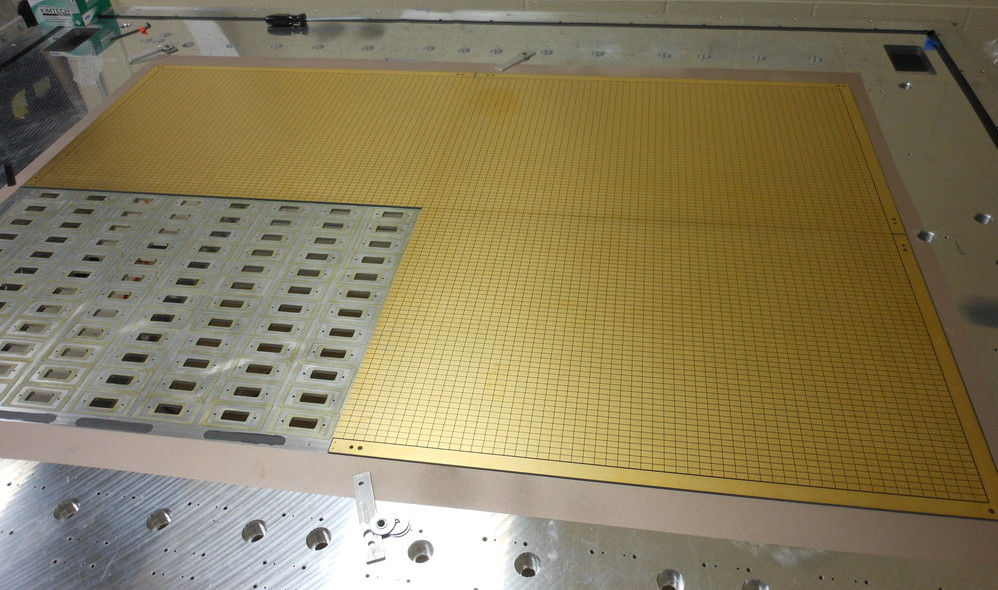
\includegraphics[width=\textwidth]{3boards_ps.jpg}
\caption{Figure of the pad plane boards being glued to the top plate. }
\label{fig:padplane}
\end{figure}


\subsection{Electronics}

Signals in the S$\pi$RIT TPC are amplified and digitized by the recently developed Generic Electronics for TPCs (GET) \cite{get}.  Short cables transmit the signals from the surface mount connectors, through a circuit protection board called ZAP, to the inputs of the AGET chips which are mounted to the AsAd board as seen in Fig.~\ref{fig:getzap}. Each AGET chip services 64 pads (63 pads are connected in our case). Four AGET chips are mounted on one AsAd  motherboard. Figure~\ref{fig:aget} is the schematic of each  AGET chip which contains a charge sensitive pre-amplifier, several other stages of amplifiers, and a Switched Capacitor Array (SCA) with a maximum of 512 time buckets which operates in a circular readout buffer. The sampling frequency can be adjusted from 1 to \SI{100}{\mega\hertz}. The gain of each AGET can be configured as 0.12, 0.24, 1.0, or \SI{10}{\pico\coulomb} over the whole dynamic range, and the analog-to-digital converters (ADCs) on each AsAd board provides 12 bit resolution. The peaking times of the shaping amplifiers can be set to 69, 117, 232, 501, 720, or \SI{1014}{\nano\second}. In this experiment, the gain was set to the highest setting, 0.12 \si{\pico\coulomb}, the peaking time \SI{117}{\nano\second}, and the sampling frequency \SI{25}{\mega\hertz} (resulting in \SI{40}{\nano\second} time buckets). 

\begin{table*}[!htb]
\centering
\ra{1.3}
\begin{tabular}{@{}rr@{}}\toprule 
\multicolumn{2}{c}{GET electronics settings}\\
\midrule
ADC bit range       & 14 bits \\
Sampling frequency  & 1-100 MHz \\
Dynamic range       & .12, .24, 1.0, 10pC \\
Peaking time        & 69,117,232,501,720,1014 ns \\
Time bucket range   & 512\\
\bottomrule
\end{tabular}
\caption{Summary of range of GET electronics settings. }
\label{tb:getoverview}
\end{table*}

\begin{figure}[!htb]
\centering
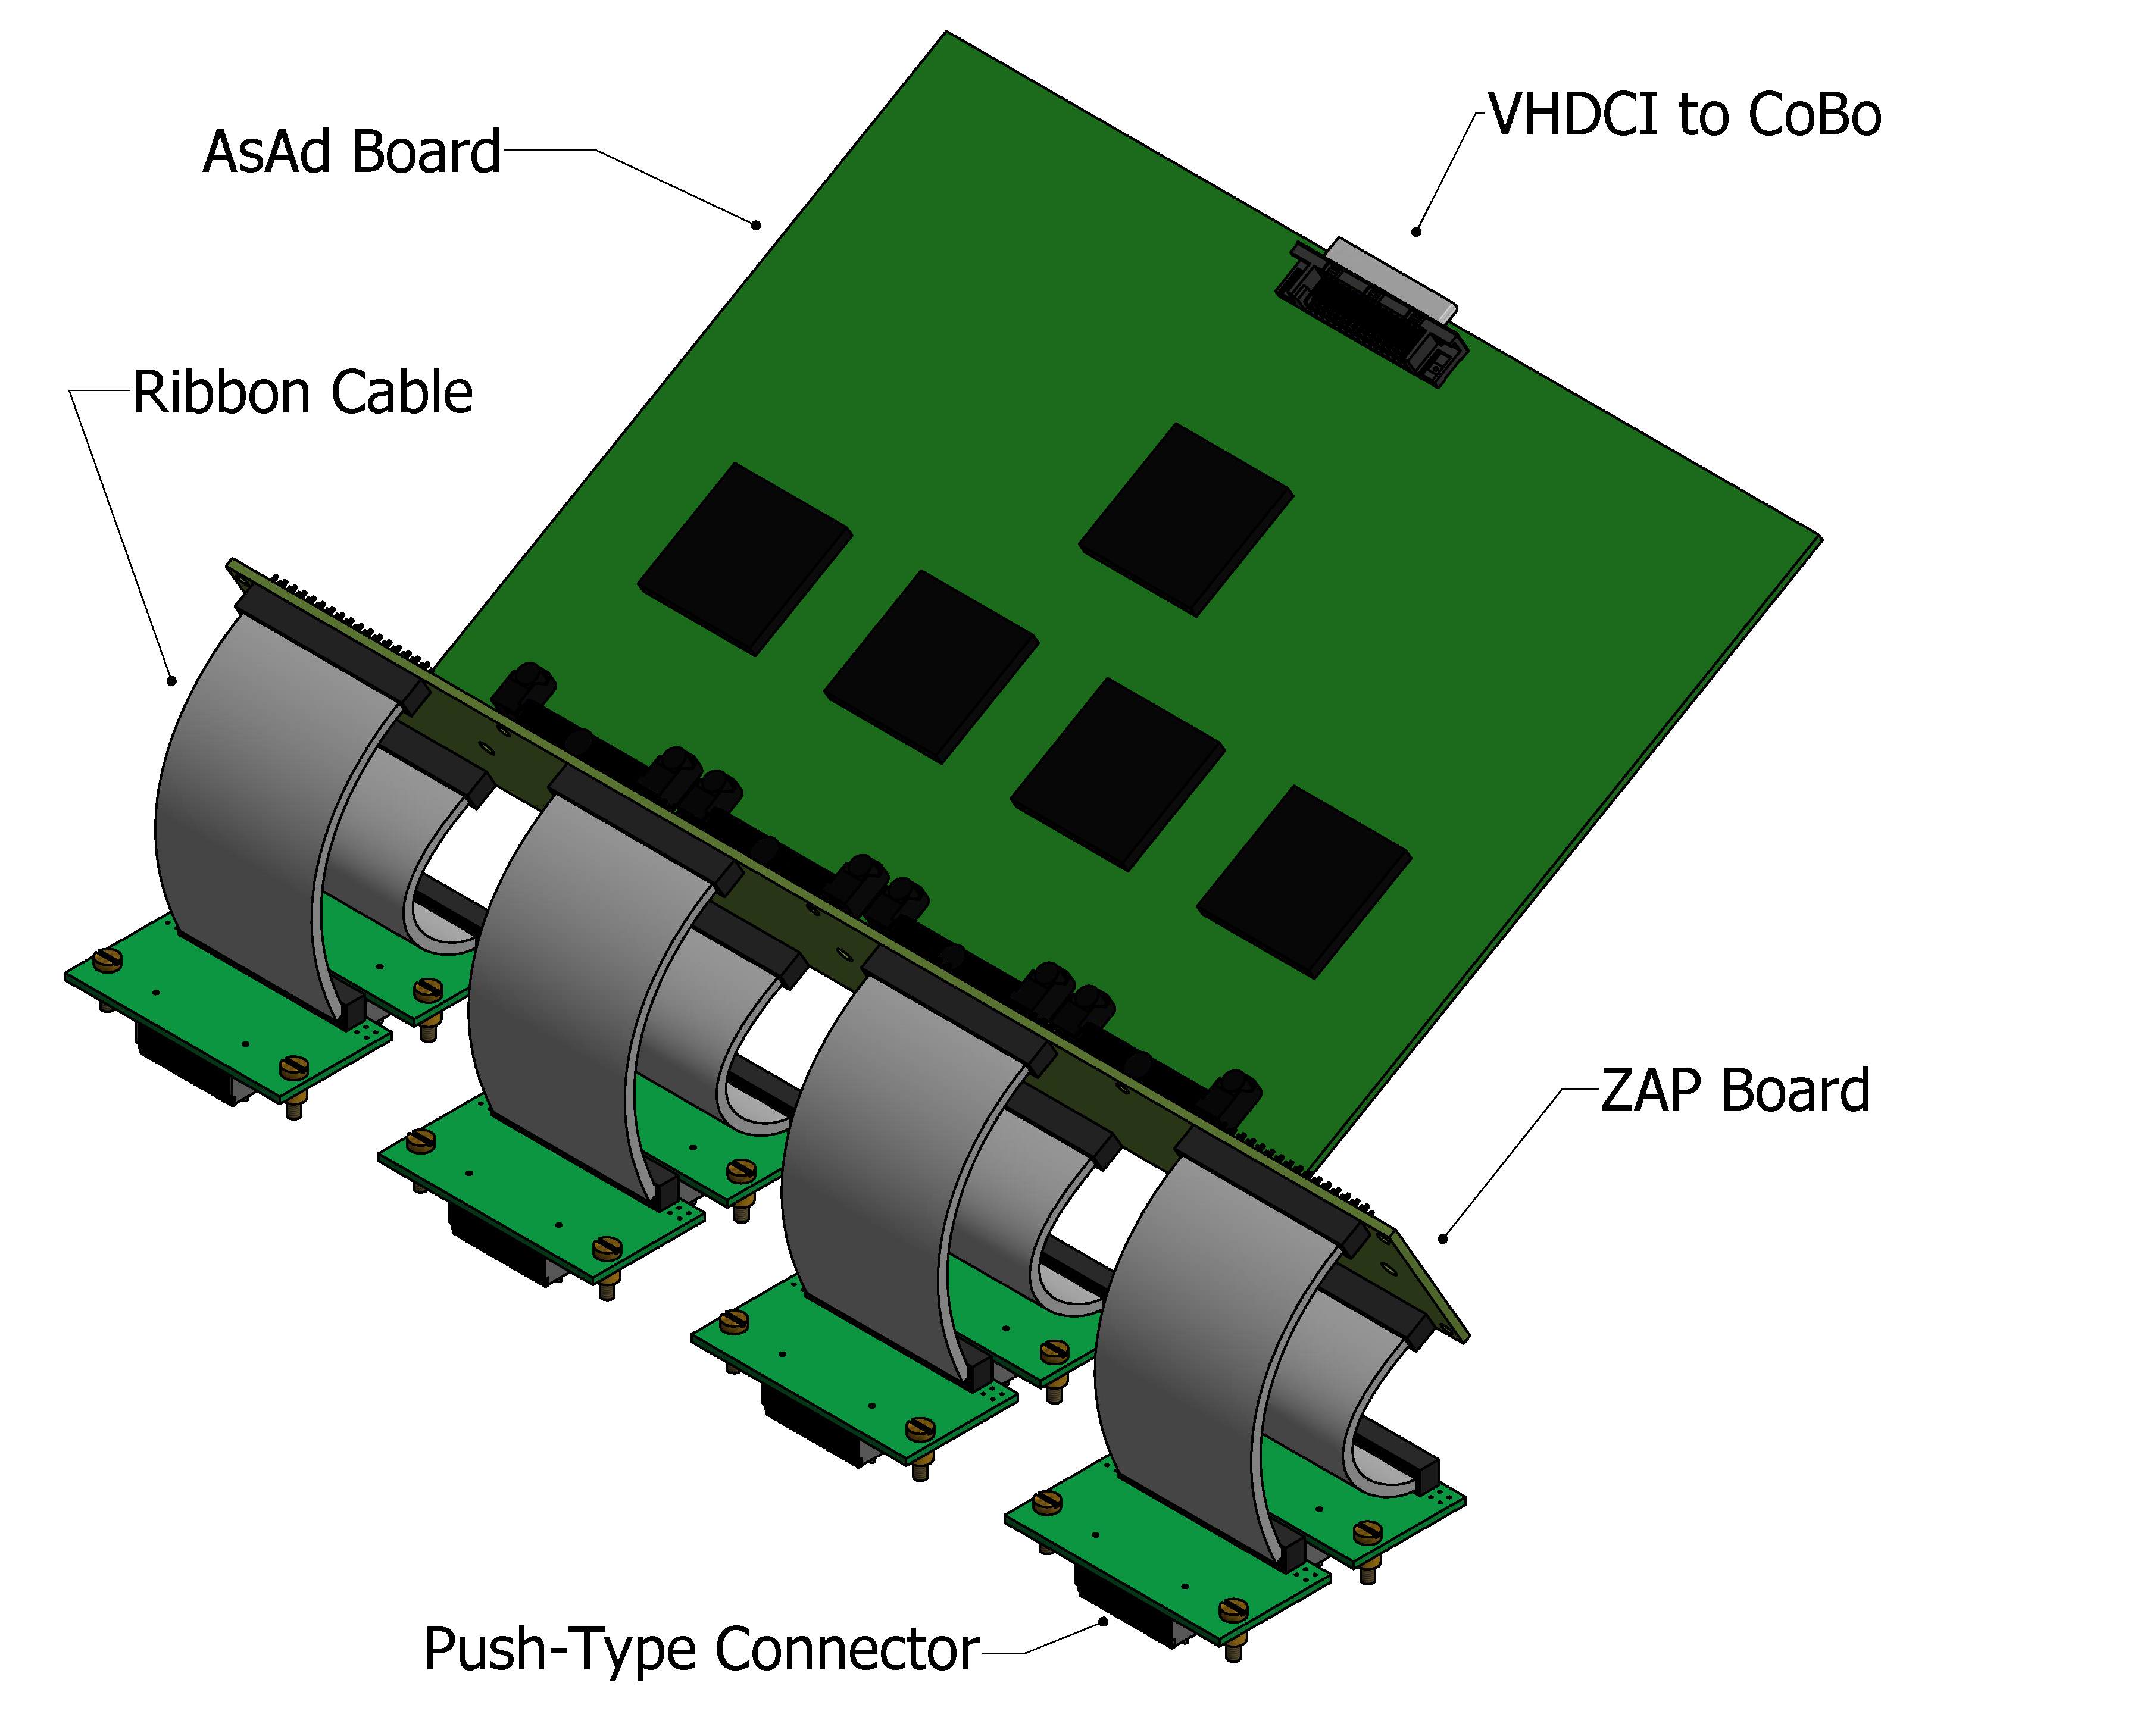
\includegraphics[width=.5\textwidth]{GET_and_ZAP.pdf}
\caption{•}
\label{fig:getzap}
\end{figure}



\begin{figure}[!htb]
\centering
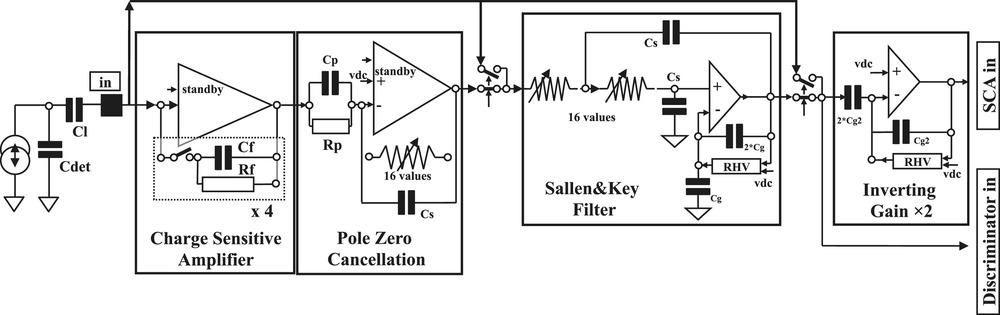
\includegraphics[width=\textwidth]{AGETfncn.jpg}
\caption{Schematic of the internals of the AGET chip from \cite{get2}}
\label{fig:aget}
\end{figure}


\begin{figure}[!htb]
\centering
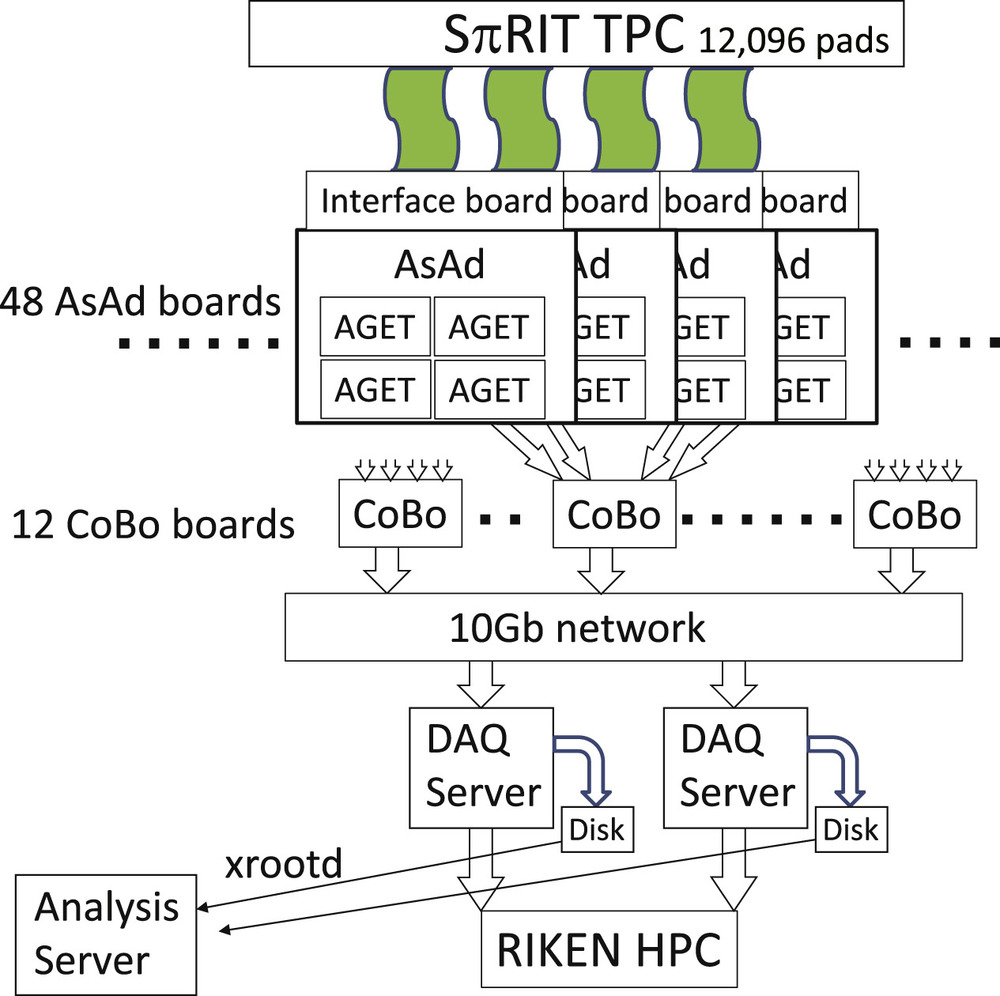
\includegraphics[width=.5\textwidth]{GETlayout.jpg}
\caption{Readout structure of the AsAd boards and CoBo board structures. Also the relevant components of the DAQ system.}
\label{fig:coboDAQ}
\end{figure}

After each AsAd board has digitized the data it is sent to the Concentration Boards (CoBo). Each CoBo board can concentrate the data from 4 AsAd boards. The Multiplicity, Trigger, and Time module (MuTanT) \cite{get} provides the common trigger signal for all CoBo boards.  Each board sends the data to the DAQ server which writes to disk the data from each board, which was handled by two separete DAQ servers; saving to one common analysis server. The data could then be analyzed using the RIKEN High Performance Computing (HPC) cluster or moved to the NSCL or MSU cluster for analysis. The Aget 2.0, asad 2.1, and cobo 1.0 firmware versions were used in this analysis. 

\section{Energy loss in material}
\label{sec:energyloss}

The average energy loss in a material can be described by the Bethe-Bloch equation,
\begin{equation}\label{eq:bb}
\frac{dE}{dx} = \frac{4\pi NZ^2e^4}{mc^2\beta^2} (ln \frac{2mc^2\beta^2\gamma^2}{I} - \beta^2),
\end{equation}
where $N$ is the number density of electrons in the medium, $e$ the elementary charge, $mc^2$ is the rest mass of the electron, $Z$ is the charge of the traversing particle, $I$ is the mean excitation energy of the medium, and $\beta$ is the velocity of the particle \cite{blumrol}. Yet there is a large variation in energy loss around this mean value. The statistical variation of energy loss in a material was described by Landau \cite{landau} and later better described by Shulek \cite{shulek} and Bichsel \cite{bichsel1}. In both approximations it is described by a most probable energy loss value, with a long, high-energy loss tail. The solid curve in Fig.~\ref{fig:straggling} shows the energy loss distribution in Ar gas for a proton with momentum \SI{3.4}{\giga\eVperc} \cite{bichsel}. The dashed line is the distribution under the Landau assumptions. The mean energy loss $\langle\Delta\rangle$ is significantly shifted from the most probable value $\Delta_p$, due to the long high energy tail.  Because of this long tail, for a finite set of energy loss measurements along a given track, the mean value is a very unreliable. The most probable energy loss is the better observable which can be obtained either through fitting of the observed distribution or through the truncated mean method. 

\begin{figure}
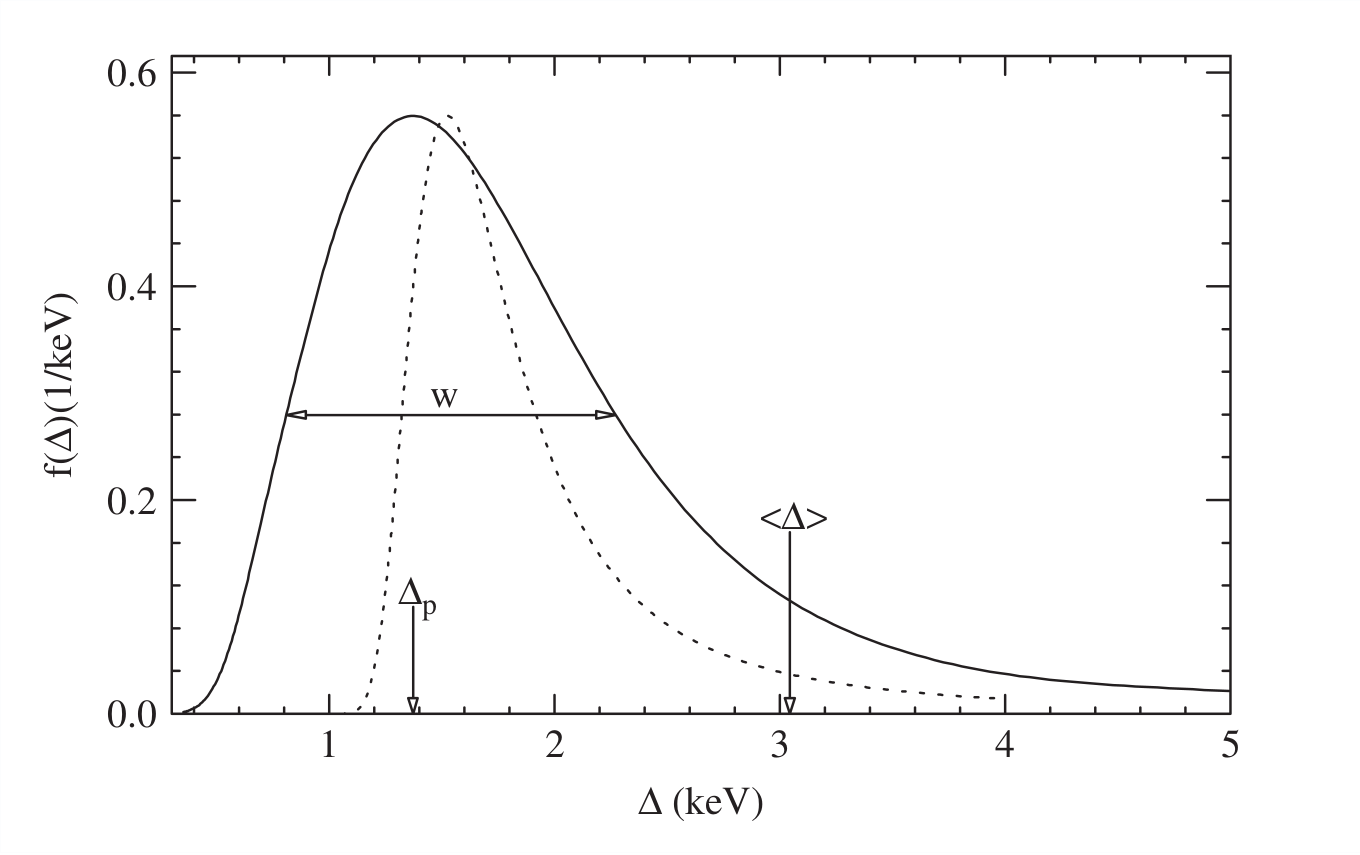
\includegraphics[width=\textwidth]{bichsel.png}
\caption{Energy loss of a $\beta\gamma$ = 3.6 particle in Ar gas taken from \cite{bichsel}}
\label{fig:straggling}
\end{figure}

The truncated mean is the average mean value calculated after throwing away the top fraction of the highest energy loss entries. This approximates the most probable value without performing a fit to a known distribution. If a set of $n$ observed energy loss values, $\Delta_i/x$, in a given track are sorted from smallest to largest value. The truncated mean $C$, is calculated from the reduced set of points $n_t = f_r n$ as,

\begin{equation}
C = \frac{1}{n} \sum\limits_{i}^{n_t} \Delta_i/x,
\label{eq:truncmean}
\end{equation}

where $f_r$ is the cut off fraction. In this thesis, a value of 0.7 was used and it was also used in the STAR TPC collaboration \cite{starsyst}. 




%Suppose $E$ represents the set of $N$ energy loss points measured, sorted from lowest to highest energy loss. The $j^{th}$ index marks the position where  $i > j$ entries represent the highest value of energy loss measurements, where their fraction of the total set is expressed as, $f_c = \sum_{i>j} E_i/ \sum_i E_i$. The truncated mean is expressed as the mean value of the remaining energy loss measurements, throwing away the top $f_c$ fraction, expressed as,

%\begin{equation}
%\langledE/dx\rangle_t = \frac{\sum_{i < j} E_i}{N}
%\label{eq:truncatedM}
%\end{equation}

 %A full description of the energy loss distribution can be described in CITE HERE.


\subsection{Gas Properties}
The gas used was a mixture of 90\% Ar and 10\% Methane ($\mathrm{CH_4}$) by volume (P10 gas), and operated just under atmospheric pressure 1 atm. The gas was continually flowed through the field cage and exited into the enclosure volume, finally passing through a bubbler to atmosphere. The gas purity was monitored with an oxygen and water monitor which are the two most concerning contaminants. The water never exceed  ??? ppm  and the oxygen level never exceeded ??? ppm. Figure~\ref{fig:driftvel} shows the drift velocity of P10 gas at 1 atm (\SI{760}{\torr}) as a function of the reduced electric field value given in units of \si{\volt\per\centi\metre\per\torr}. Operating near the peak value of the drift velocity curve minimized the change in the drift velocity as the effective field slightly changes due to slight variations in the pressure. The electric field in the experiment was \SI{125}{\volt\per\centi\per\metre} at \SI{760}{\torr}, giving a reduced electric field \SI{0.17}{\volt\per\centi\metre\per\torr}.

\begin{figure}[H]
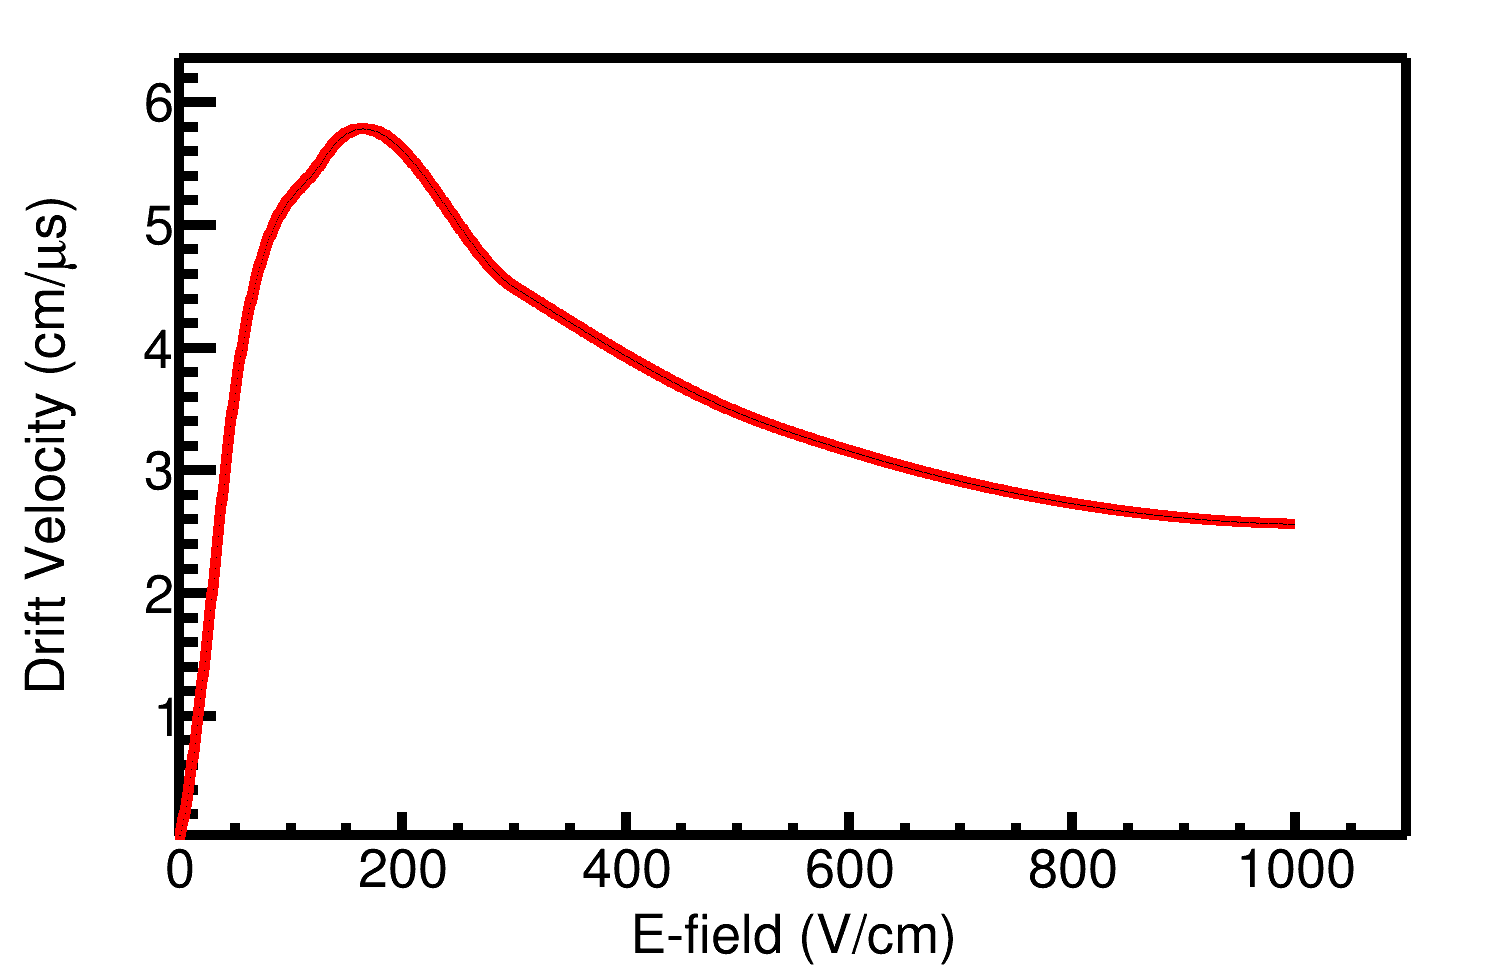
\includegraphics[width=\linewidth]{driftvel.png}
\caption{Drift velocity of electrons in P10 gas.}
\label{fig:driftvel}
\end{figure}

The general formula for the drift velocity, $d\vec{x}/dt$, of an electron in the presence of electric and magnetic fields, $\vec{E}$ and $\vec{B}$, can be expressed in the Langevin equation as,  

\begin{equation}
\frac{d\vec{x}}{dt} = \frac{\mu}{1+(\omega\tau)^2}\Big(\vec{E} + \omega\tau\frac{\vec{E}\times\vec{B}}{|\vec{B}|}+\omega^2\tau^2\frac{\vec{E}\cdot\vec{B}}{|\vec{B}|^2}\vec{B}\Big),
\label{eq:elecdrift}
\end{equation}

where $\mu=\SI{5.43}{\centi\metre\per\second}$ is the signed drift velocity, $\omega=\SI{8.79e10}{\radian\per\sec}$ is the cyclotron frequency, and $\tau=\SI{2.48e-11}{\second}$ is the collision parameter for a particular gas \cite{blumrol}.

Several properties of the gas were simulated in Garfield including the longitudinal and transverse diffusion, $\sigma_l$ and $\sigma_t$ respectively, and the electron and ion drift velocities, $v_d$ and $v_i$ respectively for the experimental electric field of \SI{125}{\volt\per\centi\metre}. The results are summarized in Table~\ref{tb:gasprop}.


\begin{table}[!htp] % not just 'h!'
\centering % not a center environment
\begin{tabular}{
  @{}
  l
  S[table-format=1.2]
  S[table-format=1.2]
  S[table-format=1.2]
  S[table-format=1.2]
  S[table-format=5.2]
  S[table-format=5.2]
  @{}
}
\toprule
Gas properties &
 {$\sigma_{t}$} &
 {$\sigma_{l}$} &
 {$v_{d}$} &
 {$v_{i}$}  &
 {$G_{h}$} &
 {$G_{l}$} \\
&
  {($\si{\centi\meter}^{-1/2}$)} &
  {($\si{\centi\meter}^{-1/2}$)} &
  {(\si{\centi\meter\per\micro\second})} &
 {(\si{\centi\meter\per\micro\second})} \\

\midrule
\phantom{abc}   &.024   &.034  &5.43  &  \num{2.05e-4} &  903   &150     \\
\bottomrule
\end{tabular}

\caption{}
\label{tb:gasprop}
\end{table}

%Add table for gas diffusion 

\section{Pad Response Function}
\label{sec:prf}
Each electron avalanche produces an two-dimensional image charge on the pad plane, as shown in the cartoon in Fig.~\ref{fig:2DPRF}, where the projection of the charge distribution onto the $x$ and $z$ axis of this distribution are labeled as $\rho(x)$ and $\rho(z)$ respectively. If $\rho(x,z)$ represents the charge distribution on the pad-plane, the total charge observed a particular pad, $Q$, is expressed as,

\begin{equation}
Q(x_o,z_o) = \int_{z_o - \frac{l}{2}}^{z_o + \frac{l}{2}} \int_{x_o - \frac{w}{2}}^{x_o + \frac{w}{2}} \rho(x-x_o\textprime,z - z_o\textprime) dxdz,
\label{eq:prfpadCharge}
\end{equation}

where $x_o$ and $z_o$ represent coordinates of the center of that pad, $x_0\textprime$ and $z_o\textprime$ are the coordinates of the avalanche, $w$ is the width, and $l$ is the length of the pad. The total charge observed for a given track is a superposition of all avalanches on all the anode wires. Typically in a TPC, the charges on each pad are grouped into clusters, and it is practical to cluster in only one direction. Therefore we will speak about the marginal probability distribution over a given layer of pads (x-distribution), or row of pads (z-distribution). The marginal distribution for a given layer can be written as,
\begin{equation}
\rho_x(x) = \int_{z_o - \frac{l}{2}}^{z_o + \frac{l}{2}} \rho(x,z)dz,
\end{equation}

and over a given row can be written as,

\begin{equation}
\rho_z(z) = \int_{x_o - \frac{w}{2}}^{x_o + \frac{w}{2}} \rho(x,z)dx.
\end{equation}

By substituting the variables  $\lambda_x = x - x_o\textprime$, and $\lambda_z = z - z_o\textprime$, we can express the charge distribution independent of the avalanche location. The Pad Response Function (PRF) along the x-direction of a given layer can be written as,

\begin{equation}
P_X(\lambda_{x_o}) = \frac{ \int_{\lambda_{x_o}-\frac{w}{2}}^{\lambda_{x_o} + \frac{w}{2}} \rho_x(\lambda_x)d\lambda_x } {\int_{-\infty}^\infty \rho_x(\lambda_x)d\lambda_x     },
\label{eq:prflayer}
\end{equation}

where $\lambda_{x_o} = x_o - x_o\textprime$; in a similar manner for the situation we cluster along the z-direction  of a given roaw the PRF can be written as,

\begin{equation}
P_Z(\lambda_{z_o}) = \frac{ \int_{\lambda_{z_o}-\frac{l}{2}}^{\lambda_{z_o} + \frac{l}{2}} \rho_z(\lambda_z)d\lambda_z }{\int_{-\infty}^\infty \rho_z(\lambda_z)d\lambda_z  },
\label{eq:prfrow}
\end{equation}

where $\lambda_{z_o} = z_o - z_o\textprime$.


\begin{figure}[!htb]
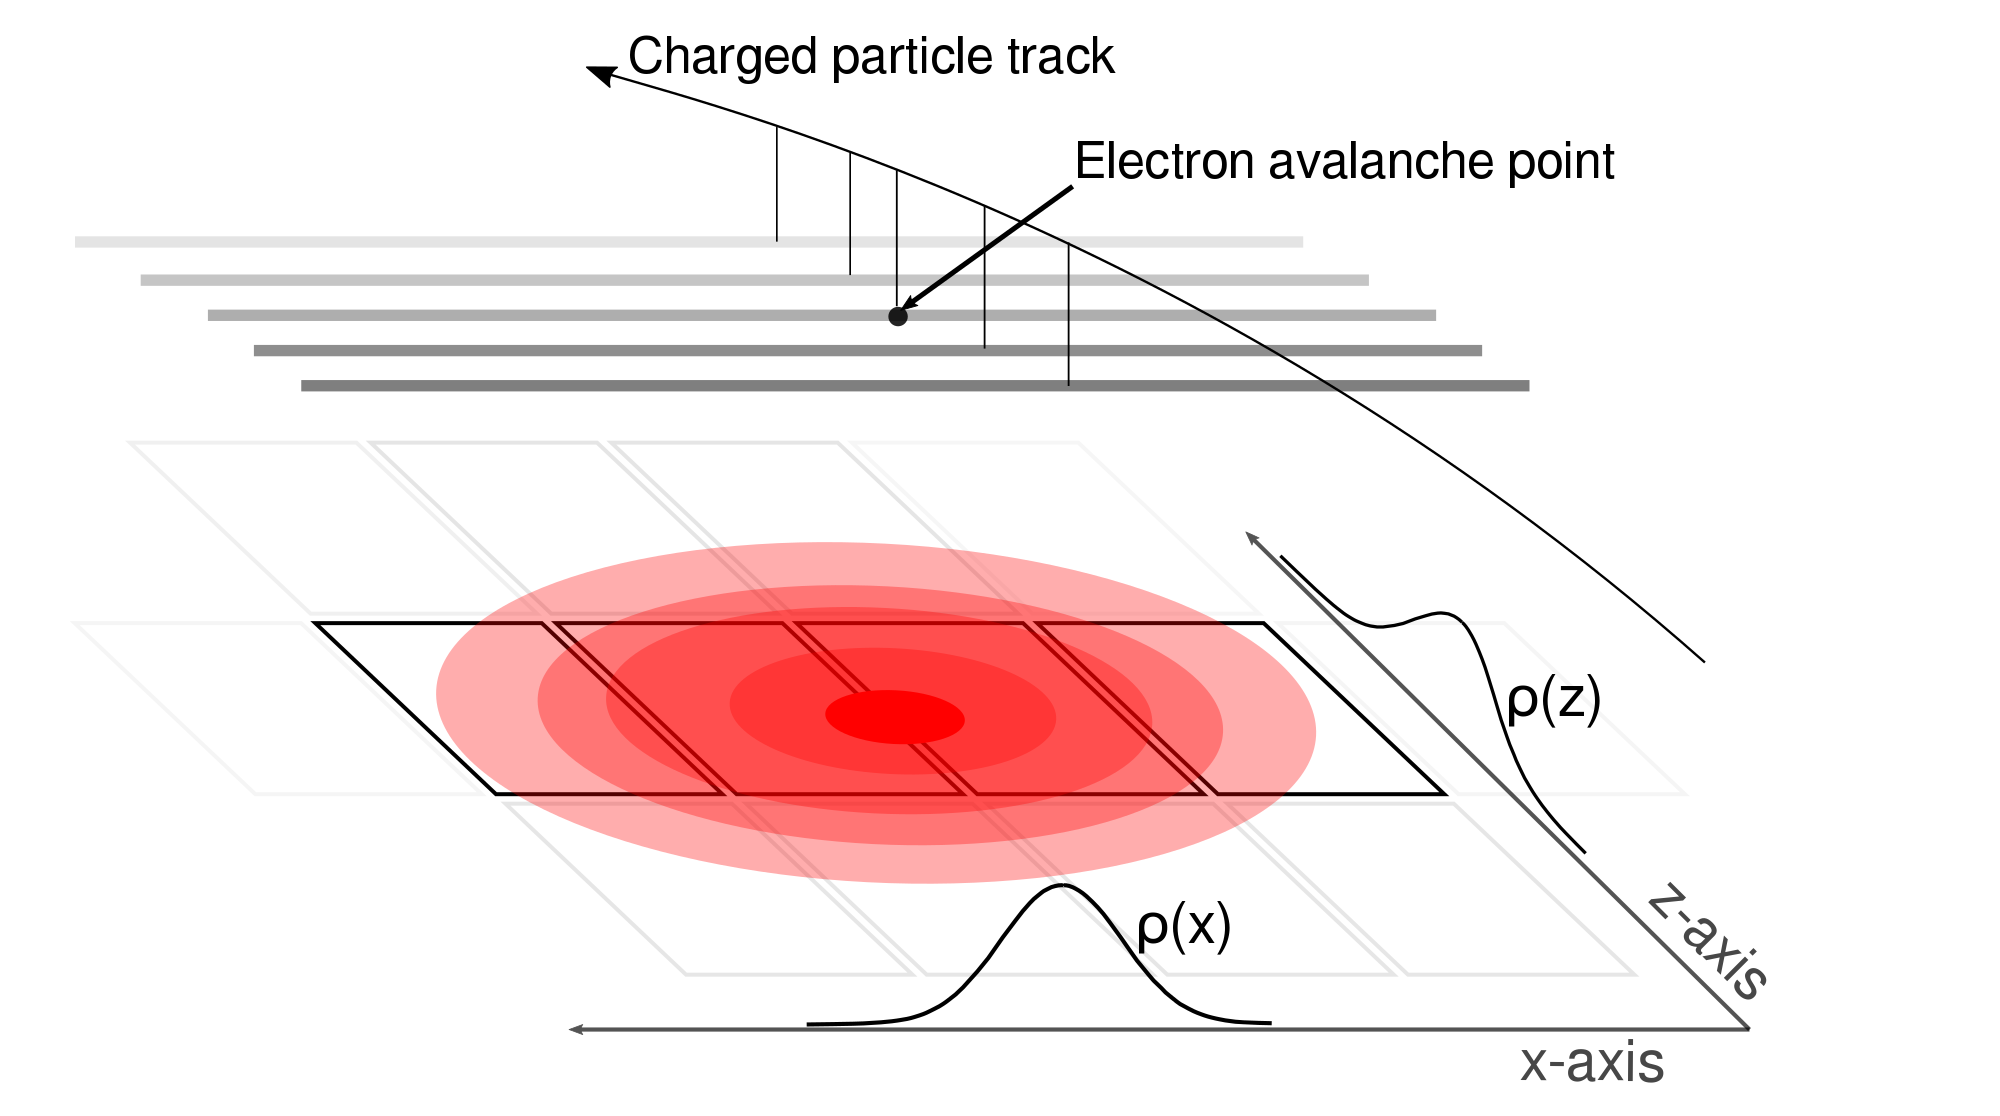
\includegraphics[width=\linewidth]{padsat_Large}
\caption{A cartoon illustration of the charge distribution resulting from an electron avalanche on one wire and the projections of the distribution onto the two axis $\rho(x)$ onto the x-axis and $\rho(z)$ onto the z-axis. The orientation of the wire planes is flipped upside down to display the perspective better.}
\label{fig:2DPRF}
\end{figure}

Gatti \cite{gatti} derived a semi-empirical formula for the charge distribution in a simple multi-wire TPC given as, 
\begin{equation}\label{eq:gatti}
\begin{split}
PRF_{\mathrm{Gatti}}(\lambda)
& = \frac{K_{1}}{K_{2}\sqrt{K_{3}}}\bigl[\arctan(\sqrt{K_{3}}\tanh\bigl[K_{2}\bigl(\frac{\lambda}{h}+\frac{w}{2h}\bigr)\bigr]) \\
& - \arctan(\sqrt{K_{3}}\tanh\bigl[K_{2}\bigl(\frac{\lambda}{h}-\frac{w}{2h}\bigr)\bigr])\bigr] \\
\end{split}
\end{equation}

where $w$ is the width of the pad, $h$ is the distance of the anode plane to the pad plane, and $\lambda$ is the distance of the pad center to the avalanche point. It is a single parameter equation where the two parameters $K_1 = \frac{K_{2}\sqrt{K_3}}{4 \arctan(\sqrt{K_3})}$ and $K_2 = \frac{\pi}{2}\left(1-\frac{\sqrt{K_{3}}}{2}\right)$ depend on the parameter $K_3$, which is a function of the ratio of the anode wire diameter to the distance of the anode wires to the pad plane. $K_3$ can be looked up in a graph in \cite{blumrol} and \cite{gatti}.


\begin{figure}[!htb]
\begin{overpic}[width=\linewidth]{fig5.pdf}
\put(61,55){\contour{white}{ PRF${}_{\mathrm{Gaus}}(\lambda)$ eq. \ref{eq:gaus}  }}
\put(61,49){\contour{white}{ PRF${}_{\mathrm{Gatti}}(\lambda)$ eq. \ref{eq:gatti} }}
\end{overpic}
\caption{Experimental pad response function of many events for a crossing angle of $85^{\circ} < \theta \leq 90^{\circ}$.  }
\label{fig:expprf}
\end{figure}


Since we take the marginal distributions only along one layer or row of pads, correlations are introduced in the PRF from adjacent layers or rows which cause slight deviations from the expected Gatti distribution. Also, analytic PRFs only exist for classical multi-wire TPCs. For these reasons it is useful to experimentally measure the PRF and fit it with an empirical function, typically a Gaussian, to describe its behavior. The method for extracting the experimental PRF will be discussed latter, but by averaging over many events in the experimental data, the resulting PRF for the S$\pi$RIT TPC is shown in Fig.~\ref{fig:expprf}. Here we see the deviations from the expected analytic Gatti distribution (black curve), whereas fitting with a two parameter Gaussian function (red curve) gives a better description of the  data, Eq.~\ref{eq:gaus}, with the two parameters being the normalization coefficient, $N_0$, width $\sigma$, and with a mean value assumed to be 0.

\begin{equation}\label{eq:prfgaus}
PRF_{\mathrm{Gaus}}(\lambda) = N_0 e^\frac{-\lambda^2}{2\sigma^2}
\end{equation}

While the differences between the Gaussian distribution and the Gatti distribution are small for this TPC geometry, we use the Gaussian distribution because of its superior reproduction of the tails of the pad response function.   



\begin{comment}
\subsection{Considerations when constructing a TPC}
Several considerations went into the construction of the S$\pi$RI TPC which I wish to summarize and document here. All materials and glues of the TPC were selected as low out-gassing materials. Several materials (that are common place in nuclear labs), such as vacuum grease, viton o-rings, all out-gas organic chemicals into the counter gas which damage the TPC by permanently lowering the gain over time. The organic molecules responsible are difficult to identify exactly, but lists of good and bad materials are well known in the literature from experiments. If a material we wished to used was not on these lists we placed the material in a clean chamber with the counter gas and flowed this counter gas through a small proportional counter making sure the gain did not drop at high collection rates when exposed to a high rate alpha Americium source. 

Sparking
Two volumes of gas. 
\end{comment}


\section{Radio Isotope Beam Factory (RIBF) Facility }
%Cyclotron facility overview.
%Samurai line overview.
%Beam line element overview.
%Big rips beam PID. reference 
The primary and secondary beams were produced at the Radioactive Isotope Beam Factory (RIFB) facility at RIKEN, in Wako-shi, Japan. The RIBF facility starts with two primary beam types, ${}^{132}$Xe and ${}^{238}$U, which are produced by an ion-source and accelerated to progressively higher kinetic energies by 1 linear accelerator (RILAC), and 4 different cyclotrons (RRC, fRC, IRC, and SRC), until they reach a beam energy of \SI{345}{\MeVA}. Figure~\ref{fig:samuraiBeamLine} shows the later stages of the cyclotrons and the following beam lines to which these beams can be sent. For this dissertation, the beam went through the BigRIPS spectrometer, where the specific rare isotope beams of interest were produced and on to the SAMURAI dipole where the  \spirit TPC was placed. The red box indicates the location of the experimental setup in Figure~\ref{fig:samuraiBeamLine} .


\begin{figure}[!htb]
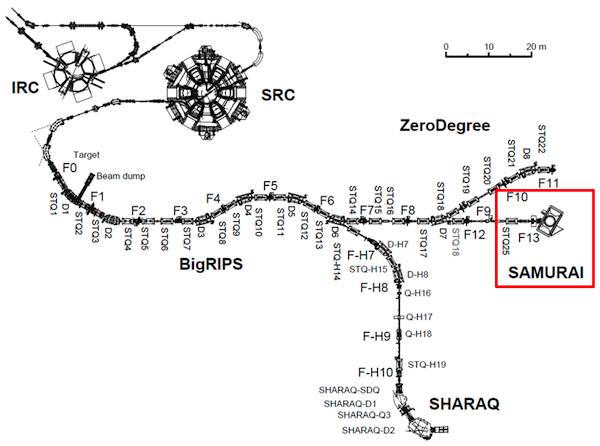
\includegraphics[width=\linewidth]{SAMURAI-beamline.png}
\caption{Overview of the RIBF, BigRIPS, and SAMURAI beamline.}
\label{fig:samuraiBeamLine}
\end{figure}

After the SCR, the primary beams impinge on a rotating \SI{3}{\milli\metre} Be target which fragments the beam into many different species. These fragments are then separated by the BigRIPS spectrometer which is tuned to the particular secondary fragment of interest. This is accomplished through several dipole magnets, slits, and wedge degraders. The resulting secondary beam is not pure and the purity depends on the capability of BigRIPS to deliver the secondary beam of choice and the primary beam used. The BigRIPS separator had many scintillators for timing, an ion chamber for Z identification and beam tracking elements used to determine the magnetic rigidity of the beam. Information from these detectors allow  allowed  identification  of the mass, charge and momentum of each isotope in the secondary beam. This information was determined beam particle by beam particle and recorded along with the TPC data on each event. With this information, it was possible to select with precision the reactions to be included in any subsequent data analysis.  

In the experimental campaign,   several beams were utilized that have  different intensities and purities. Table~\ref{tb:beams} summarizes the average qualities of the 4 secondary beams that were used in our experimental campaign. Most beams were delivered with an intensity of \SI{10}{\kilo\hertz}.

 \begin{table*}\centering
\ra{1.3}
\begin{tabular}{@{}ccccc@{}}\toprule 
 Primary Beam & Secondary Beam & Energy at mid target \si{\MeVA} & Intensity \si{\kilo\hertz} & Purity (\%) \\ [0.5ex] 
 \midrule
 ${}^{238}$U   & ${}^{132}$Sn   &  269.2  &  9.5  &  54   \\
 ${}^{238}$U   & ${}^{124}$Sn   &  270.3  &  9.1  &  10  \\
 ${}^{124}$Xe  & ${}^{112}$Sn   &  270.4  &  7.6  &  48  \\
 ${}^{124}$Xe  & ${}^{108}$Sn   &  269.3  &  7.5  &  52   \\
 \bottomrule
\end{tabular}
\caption{Primary and secondary beam properties produced in the \spirit TPC experimental campaigns. }
\label{tb:beams}
\end{table*}



\section{Experimental Setup}

The \spirit TPC was designed to fit exactly into the dipole gap of the  dipole magnet at the end of the BigRIPS beam line. Figure~\ref{fig:experiment} shows a drawing of the \spirit TPC inside of the SAMURAI magnet chamber which was rotated to the $\ang{0}$ configuration. Typically the SAMURAI (Superconducting Analyzer for Multi-particles from Radioisotope beams) dipole magnet is operated under vacuum as a large-acceptance multi-particle spectrometer for radioactive-beam experiments. This magnet can reach magnetic fields up to \SI{3}{\tesla} at the center of the pole gap and was operated at \SI{0.5}{\tesla} for these sets of experiments. The space between the magnetic pole faces is further complicated by large bolts which protrude from the pole faces. These bolts secure the vacuum chamber to the magnet which is not practically removable; though the inside of the magnet was not operated under vacuum. This required an extensive rail system and support frame to slowly slide in the TPC over the bolts, finally raising the TPC several \si{\centi\metre} to the final height. 

\begin{figure}
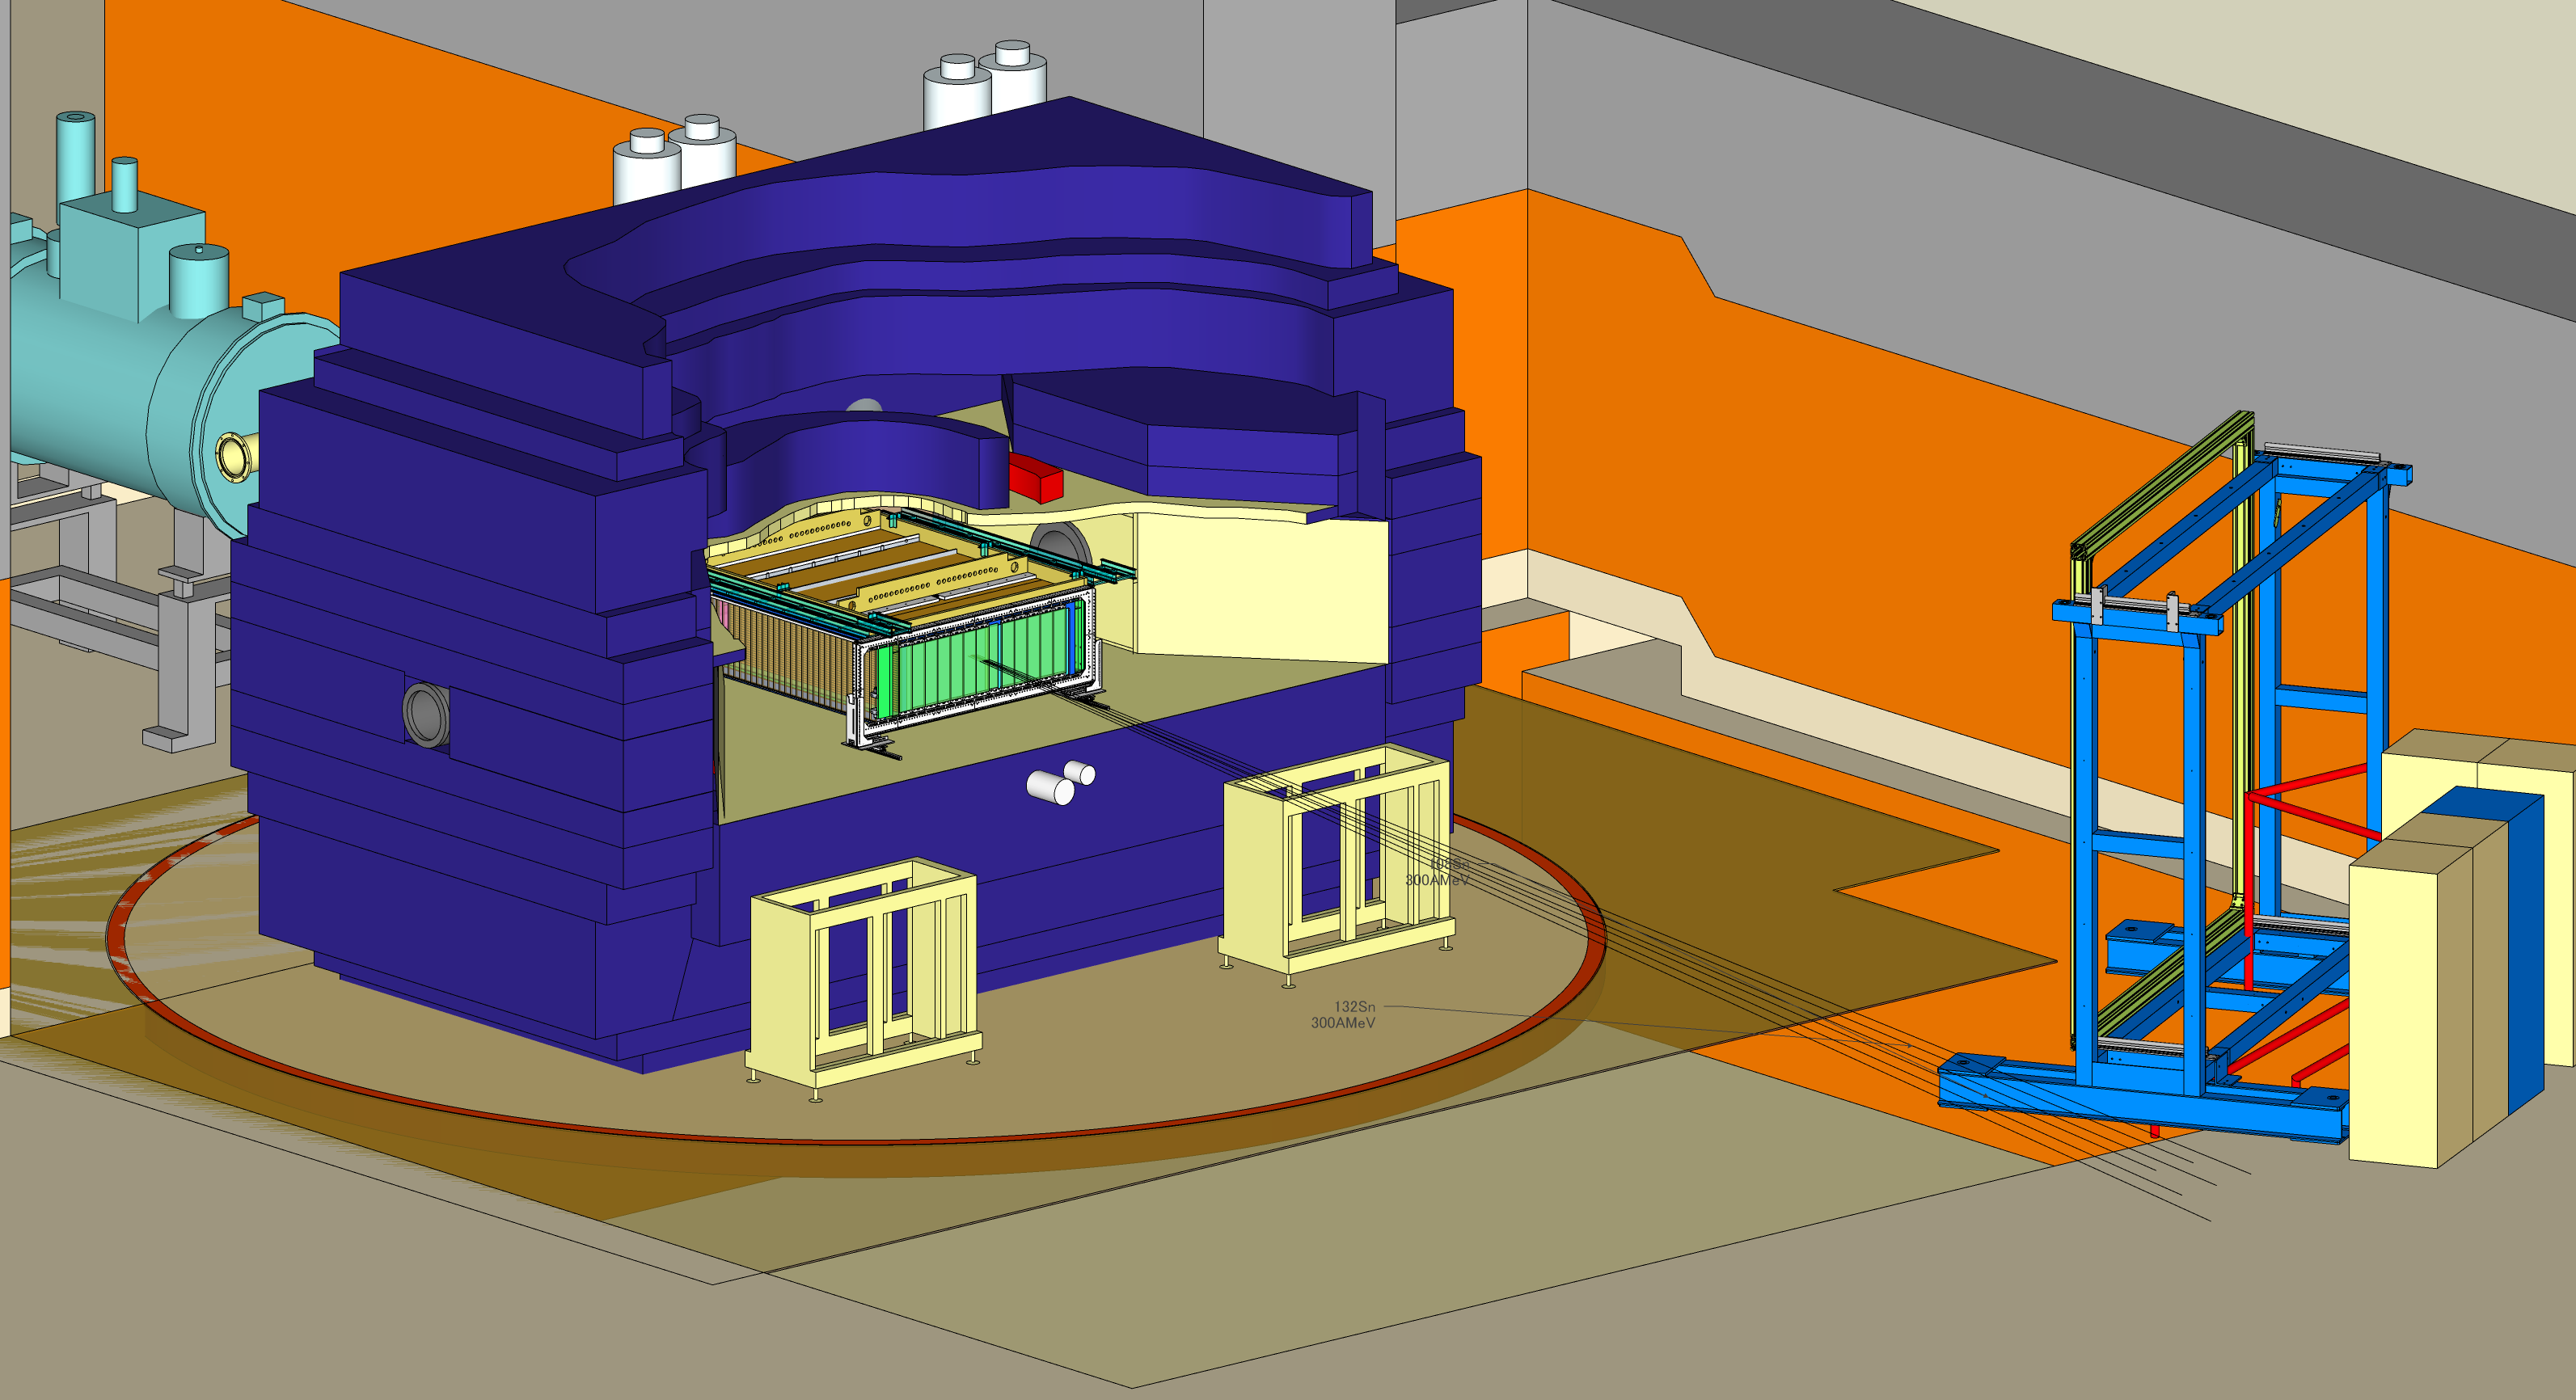
\includegraphics[width=\textwidth]{perspective.png}
\caption{Drawing of the experimental setup with the TPC inside of the SAMURAI magnet at $\ang{0}$ configuration.}
\label{fig:experiment}
\end{figure}

The height of the TPC was roughly aligned with a self-leveling laser system to match the center of target with the center of the beam line. Once the TPC was adjusted to the final location, the position of the TPC was measured in fine detail with a the VStars-N photogrametry system \cite{vstars}. Small highly reflective targets were placed all over the TPC both inside and out and pictures were taken with a calibrated lens and camera system. Using the commercial software provided the set of different camera perspectives was reconstructed into a 3-dimensional point cloud of all the targets. Since the magnet was also measured with the same system after installation, we can match the two systems to get the absolute position of the TPC, and its internal components, relative to the magnet frame. The position resolution of this type of system was estimated to be around \SI{200}{\micro\metre} for each coordinate, which is much more precise than needed or Show data.

The origin of the \spirit TPC was defined to be at the center of the TPC pad plane in the x-direction and at the edge of the last upstream pad. The center of the magnet is defined as the center of the magnet in x and z-directions and the middle of the dipole gap in the y-direction. The origin of the \spirit TPC in the magnet frame is (1.794,205.502,-580.526) for x,y,z-coordinates in units of \si{\milli\metre}. The error in each coordinate estimated to be (.2,.1,.4) \si{\milli\metre} respectively. 

%Maybe put a position table summary here of the TPC position and definition of the coordinates system in the TPC frame and the Magnet frame

\section{Beam Drift Chambers (BDC)}
\label{sec:bdc}

There were two beam drift chambers (BDC) located along the beam pipe upstream of the magnet and after the last focusing quadropole magnet. These beam drift chambers contained two sets of parallel plate avalanche counters (PPAC) which could get the (x,y) coordinates of the beam. Since they were places approximately \SI{1}{\metre} apart, we were able to track the direction of the beam in the beam line using a linear extrapolation. The resolution of the initial angle the beam enters the SAMURAI dipole was estimated to be \SI{0.64}{\milli\radian} and \SI{0.24}{\milli\radian} for the two angles defining the beam vector \cite{jon}. The initial angle, energy, and charge of the beam is then propogated through the magnetic field map until the angle on target is found. The angle on target though small will be important later for transforming back into the center of mass system as will be seen in Sections~\ref{sec:beamangle,sec:pionSpectra}.


\section{Ancillary Detectors }
Several ancillary detectors were placed inside and outside of the \spirit TPC to facilitate in making the trigger for the experiment. The ability of ancillary detectors to work effectively when placed outside the TPC  was one of the more important considerations we made when designing the TPC. A brief description of each ancillary detector system is given here with particular focus on how the experimental trigger was made. 


\subsection{Kyoto Multiplicity Trigger}
\label{sec:kyoto}
%kyoto array sets multiplicity trigger
%scintillator bars
 The Kyoto Multiplicity Array, shown in Fig.~\ref{fig:aux}, consists of two arrays of plastic scintillating bars on each side of the TPC, each consisting of 30 bars. The entire TPC structure was designed so that light charged particles could pass through the field cage and side walls of the TPC enclosure without excessive energy loss and scattering. This allowed the number of tracks passing through the sides of the TPC could be measured by in an external array. In heavy ion collisions the more central a nuclear collision is, the more nucleons participate in the collision, resulting in a higher observed track multiplicity. It is this correlation between the number of tracks and centrality of the collision that makes the number of hits in the Kyoto Array sensitive to the centrality of events. It is more likely that in very central collisions more tracks are going to the large angles and measured by the Kyoto array. In the experiment the trigger selection criteria was $n_{Kyoto} > 4$, where $n_{Kyoto}$ is the total number of tracks measured by both arrays. The Kyoto array proved to be a good trigger that suppressed peripheral collisions; this will be discussed in later sections. 

\begin{figure}[!htb]
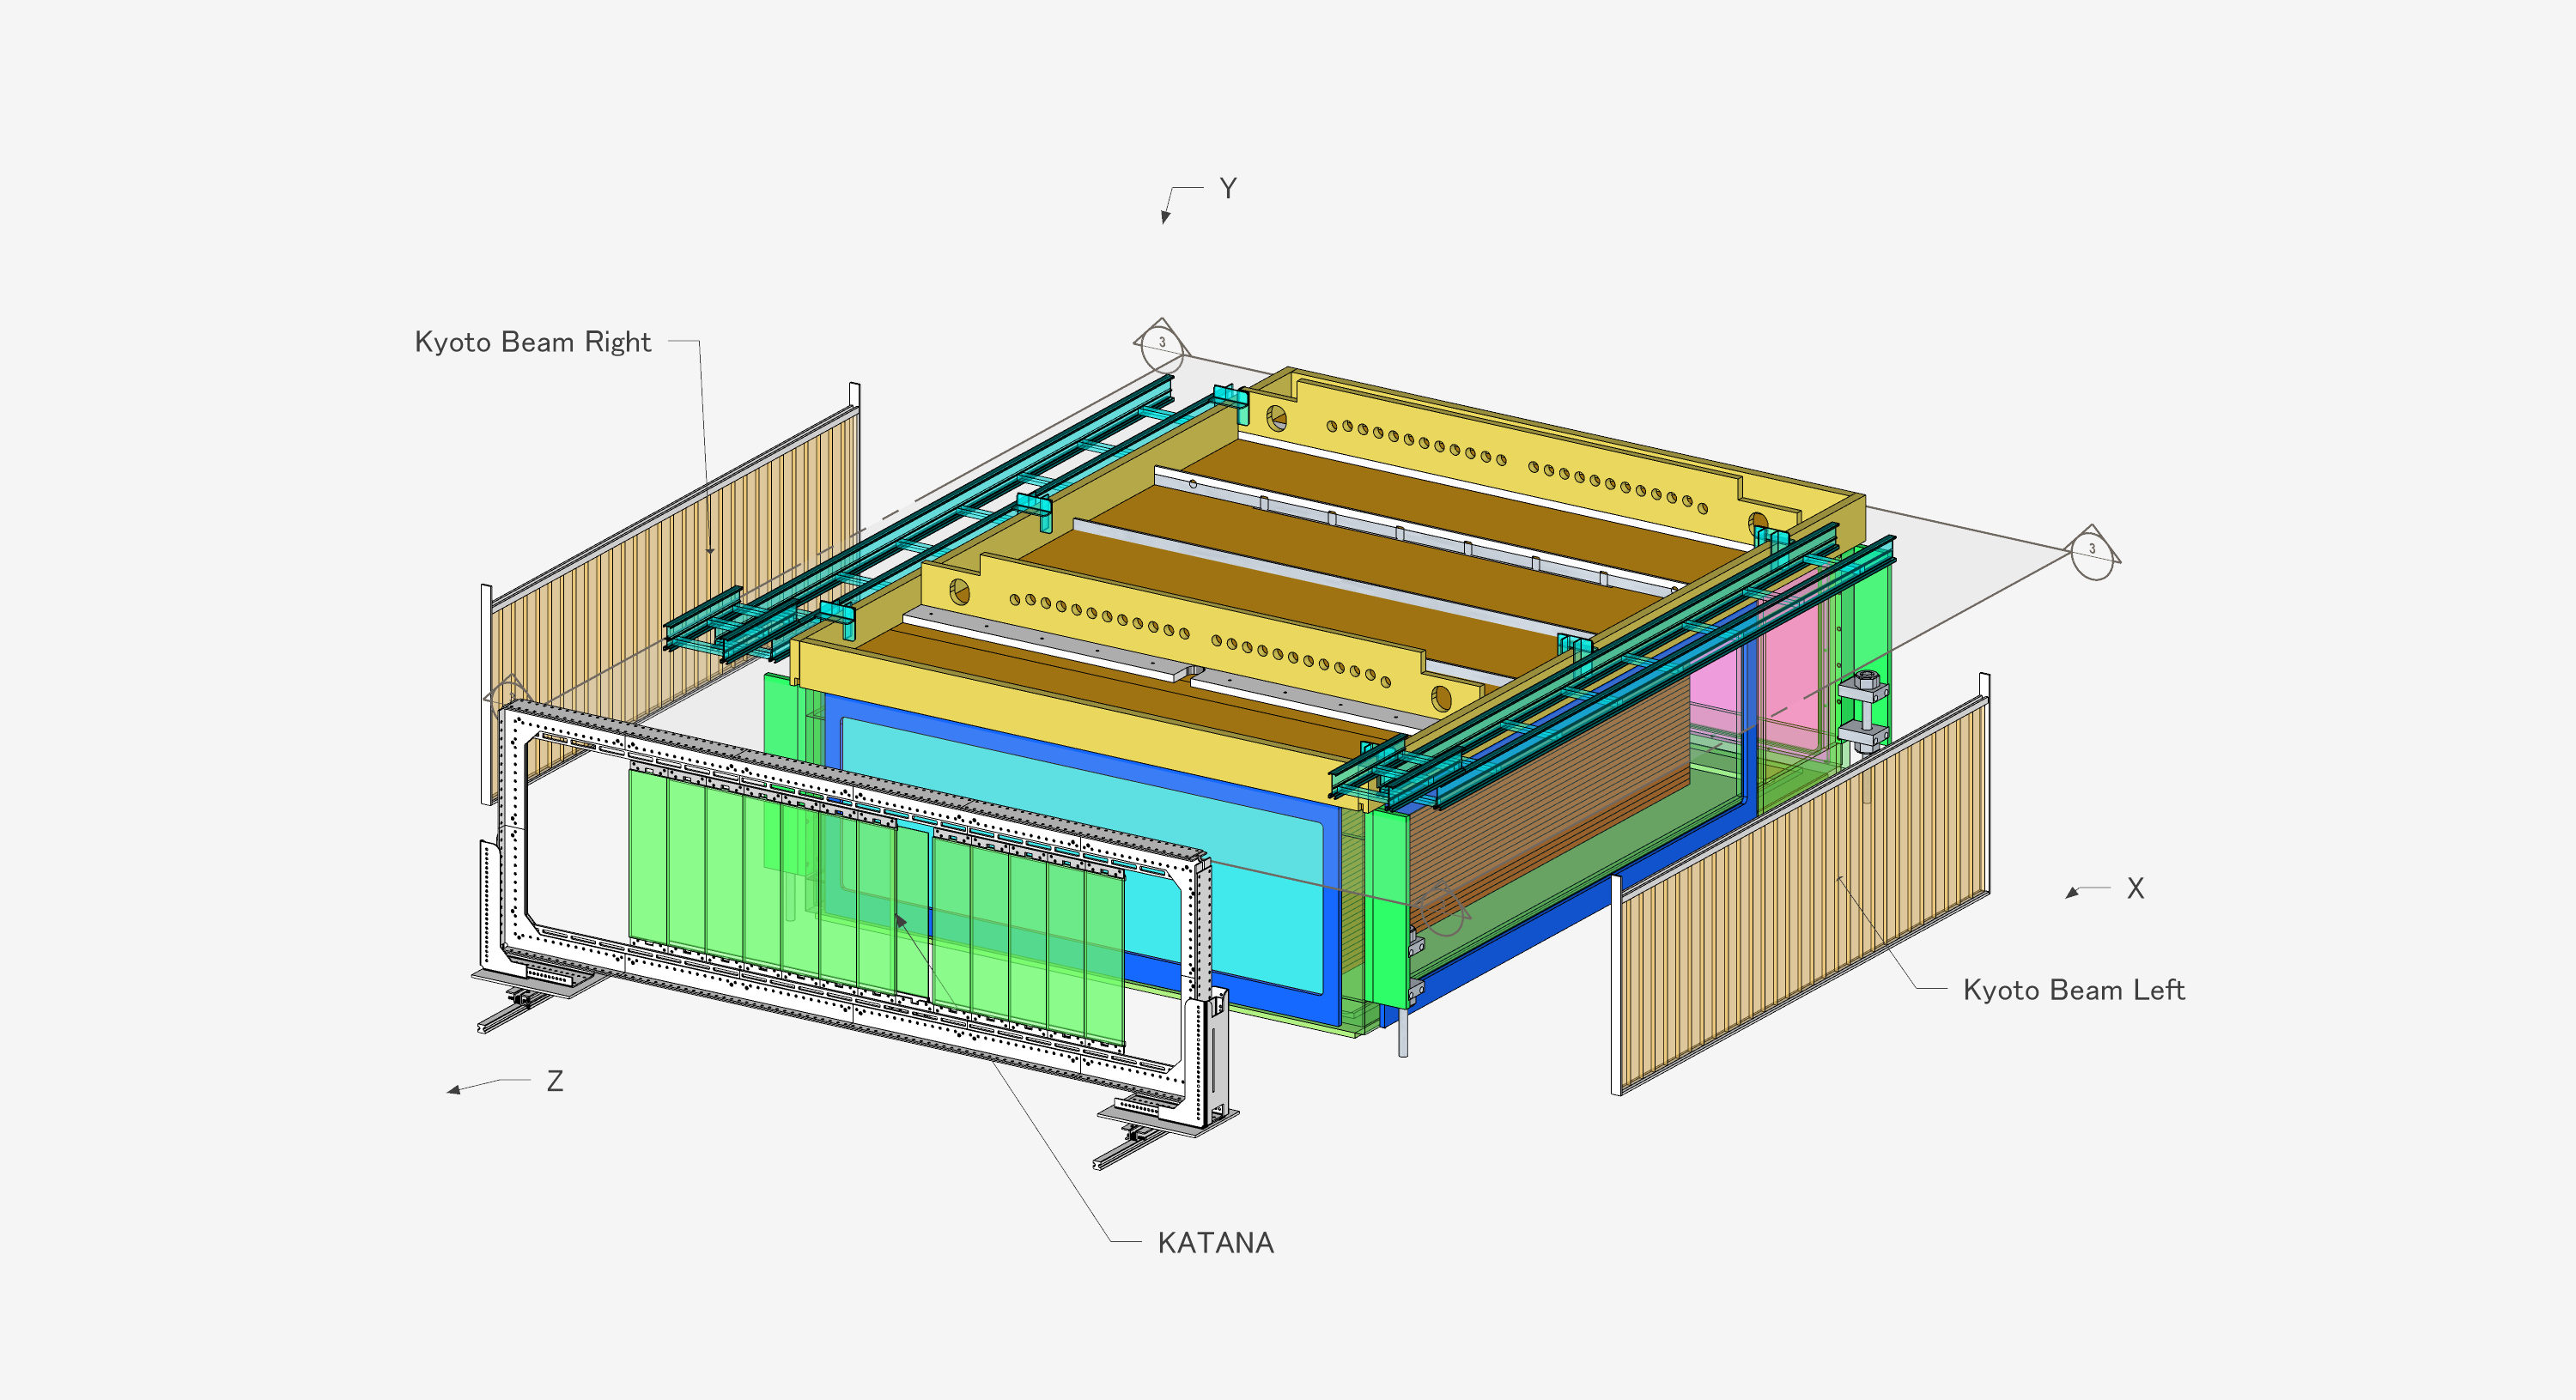
\includegraphics[width=\textwidth]{TPCAux.png}
\caption{Exploded views of Kyoto and KATANA arrays.The Kyoto array elements are in tan and are located on the left an right side of the TPC. When they are in place, they are nested against the thin aluminum side windows of the TPC. The KATANA array is in green and is located adjacent to the downstream window of the TPC.}
\label{fig:aux}
\end{figure}


\subsection{Krakow KATANA Veto and Multiplicity Array}
%beam veto
%beam trigger optional
 Fig.~\ref{fig:aux} also shows the Krakow KATANA array, which consists of 12 plastic scintillating bars mounted adjacent to the downstream wall of the TPC enclosure. Three of the 12 bars 1 mm in thickness and operated as a beam veto in the event the beam did not make a nuclear collision with the target; this occurred approximately 99\% of the time. The 9 other bars were 1 cm in thickness and provided additional information about the light particle multiplicity array similar to the Kyoto array. We found that a large number of events involved peripheral collisions and active target events in which the beam interactions with the counter gas. Active target events contributed to a large multiplicity in the KATANA but not to the Kyoto array. So multiplicity $M_{Kyoto} > 4$ in the Kyoto array combined with a veto on events with a forward going projectile remnant with Z>20 provided the most effective suppression of peripheral collisions and active target events. Thus the KATANA array was used in primarily the beam veto mode. This was accomplished by positioning the array so that the expected position of the beam exiting the TPC would be centered on the three thin paddles. The threshold of the veto paddles were set so that the charge of a particle passing through, $Z$, would veto any event that satisfied $Z > 20$, where the charge of the Sn beam is $Z=50$. 


\subsection{Active Veto Array}
The beam was tuned by two sets of quadrupole  magnets, STQ 1 and STQ2 (as seen in Fig.~\ref{fig:samuraiBeamLine}), so that the beam spot was focused on the TPC target location. Because of the inherent angular dispersion of the beam there still were incoming beam events which significantly deviated from the target location. These could be suppressed in the analyses by a gate on the reaction vertex; however, there remained a concern about the dead time such target frame events would contribute and how this would limit the amount of good data we could obtain.  To veto these type of events an active veto array was set at the entrance of the TPC consisting of four small scintillating bars arranged to be slightly larger than the target size. The threshold was set so that any beam particle which passed through any of the bars it would send a trigger signal to not trigger the system since the beam path would not be on target but on some other material inside the TPC. Minimizing these active veto rates also proved to be useful when tuning the beam so as to be centered on the target.


\section{Data Acquisition (DAQ) }
The Data AcQuisition (DAQ) consisted of three different systems. The RIBFDAQ system served as the master DAQ for the BigRIPS beam identification DAQ, the TPC DAQ, the NeuLAND neutron wall DAQ, and the Kyoto Array DAQ systems. The TPC DAQ was handled by the NARVAL framework to readout the GET electronics for the \spirit TPC. A General Trigger Operator (GTO) trigger was supplied to each DAQ synchronizing the subsystems. 

\section{Trigger Condition}
Signals from all of the auxiliary detectors were combined into several logic combinations to form a trigger logic for triggering the data acquisition  (DAQ) to record data. An upstream scintillating bar formed the start counter signal, triggering on any beam coming down the beam line. The active veto will trigger for any beam that is off the target location. The KATANA veto produced a signal if the beam passed through the TPC un-reacted, causing no nuclear collision; this produces a veto signal with a width of \SI{4}{\micro\second} which is the approximate time it takes for the beam to drift and clear the field cage volume. The Kyoto multiplicity trigger produces a signal when the total number of tracks passing through both Kyoto arrays are greater than 4. 


\begin{figure}[!htb]
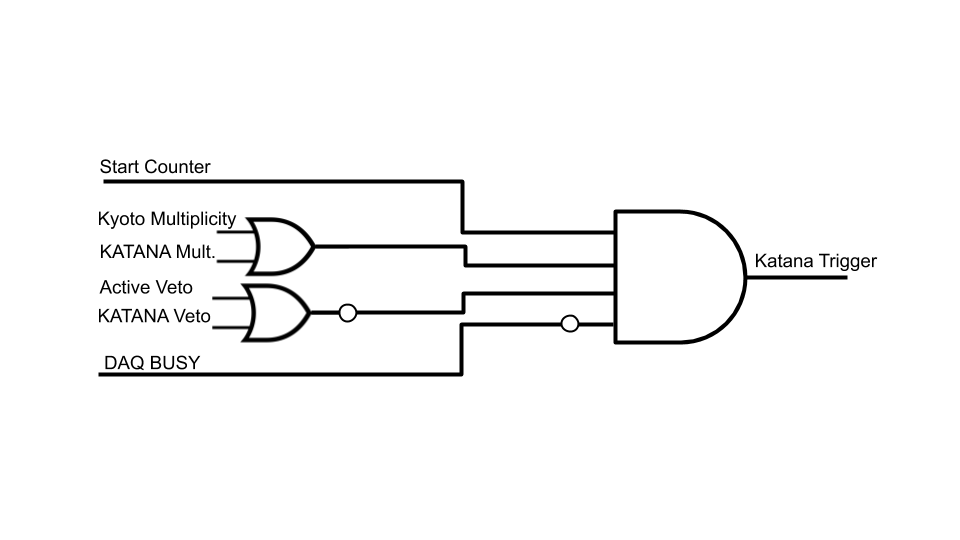
\includegraphics[width=\linewidth]{KatanaLogic.png}
\caption{KATANA trigger box logic.}
\label{fig:katanaLogic}
\end{figure}

\begin{figure}[!htb]
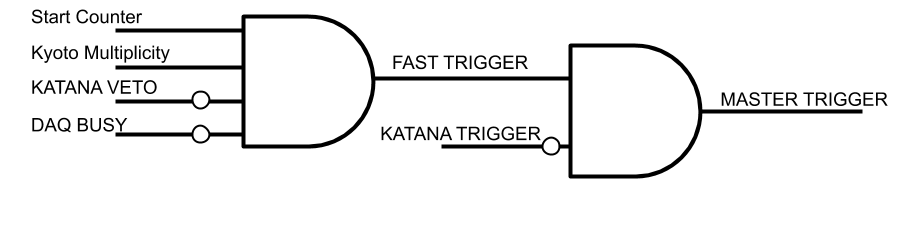
\includegraphics[width=\linewidth]{TriggerLogic.png} 
\caption{Master trigger logic.}
\label{fig:trigLogic} 
\end{figure}



\begin{figure}[!htb]
    \centering
    \begin{subfigure}[t]{0.45\textwidth}
        \centering
        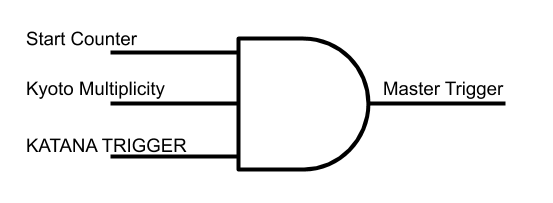
\includegraphics[width=\linewidth]{DataTrigger1.png} 
        \caption{${}^{124}$Xe primary beam trigger.} \label{fig:dataTrigger1}
    \end{subfigure}
    \hfill
    \begin{subfigure}[t]{0.45\textwidth}
        \centering
        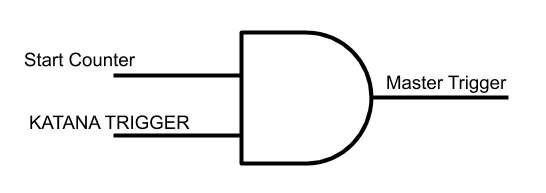
\includegraphics[width=\linewidth]{DataTrigger2.png} 
        \caption{${}^{238}$U primary beam trigger.} \label{fig:dataTrigger2}
    \end{subfigure}
\label{fig:datatrigger}
\end{figure}


There were several special trigger considerations incorporated into the trigger for the TPC. We required that the gating grid be opened quickly to not lose electrons from portions of the tracks that pass close to the gating grid. If the DAQ was not busy, we therefore generated a trigger once we had a start detector signal, a Kyoto multiplicty >4 signal, and neither a Katana Veto signal nor an active target signal. This was referred to as the Fast Trigger, and it triggered the opening of the gating grid, which took about 350 ns. Following the initial trigger, we had the possibility of a fast clear signal that could be initiated by a later beam particle traversing the TPC. If the last beam particle came within xx us after the fast trigger, electrons from this beam particle could pass through the gating grid. Such data would be useless, so we closed the gating grid and stopped the data equisition with a fast clear signal. Additional fast clears could also initiated if the Katana trigger box did not generate a trigger. Figure~\ref{fig:trigLogic} shows the logic of both of these triggers.

The Katana trigger box took some time to completely master, it did not take on the major trigger responsiblities at first. In later runs, most of the trigger functions were performed the in Katana trigger box. The master trigger for the DAQ was different for each primary beam as the experiment got progressively better. During the ${}^{124}$Xe primary beam, the KATANA trigger box was an input into the trigger logic, where as in the ${}^{238}$U primary beam, the KATANA trigger box functioned as the trigger logic utilizing the internal trigger electronics. In either case the differences in the trigger logic were very minor and they both behaved practically the same except for minor details on the gating-grid trigger \cite{jon}. Figure~\ref{fig:katanaLogic} summarizes the KATANA trigger box logic. 

Figure~\ref{fig:dataTrigger1} summarizes the ${}^{132}$Xe primary beam, where the condition to produce a true KATANA trigger output was there must be a Start Counter, KATANA multiplicity, no Veto, and no DAQ busy signal. The KATANA trigger, Kyoto Muliplicity, and Start Counter together triggered the DAQ. 

 Fig.~\ref{fig:dataTrigger2} summarizes the ${}^{132}$Xe primary beam, where the condition to produce a true KATANA trigger output was there must be a Start Counter, Kyoto or KATANA multiplicity, no Veto, and no DAQ busy signal. Here the KATANA trigger and the SC SUM??? together triggered the DAQ. 
 
 %I don't think this is true.
 
 It is worth mentioning how the busy signals for the experiment were handled. The DAQ system itself produces a busy signal which was combined in an OR with the busy signals from either the opening or closing the gating grid. When opening the gating grid, it is assumed the full volume of the TPC will be read out, therefore  a \SI{11}{\micro\second} gate busy signal is produced; which is slightly more than the time it takes for all the electrons to drift in the field cage. In the case were the gating grid should be closed, either due to the fast clear circuit or the end of the TPC measurement, a \SI{5}{\micro\second} busy signal is produced to allow for the gating grid to settle to a steady state closed configuration, and to clear the drift volume of any residual electrons from the beam. Both of these gates are included with the DAQ in an OR configuration which makes the overall busy signal. 
 


\section{Collision Data Taken}

Figure~\ref{fig:data} shows the example pad plane readout of the TPC from a central nuclear collision of Sn + Sn. Here we can see several tracks resulting from a single vertex location which is near the target region. The color values represent the max ADC observed in a given pad. The large amount of saturation that occurs in the electronics which is represented by the brightest yellow value. Also the lower voltage anode sections described in Section~\ref{sec:wireplanes} are denoted by red arrows. The pads directly over these wire planes have an effective gain reduction due to the lower anode voltage on the wires. Tracks with a high enough energy loss continue through these sections, but tracks with low energy loss values do not deposit enough energy and disappear, only to reappear in the higher gain section in between. 

\begin{figure}[!htb]
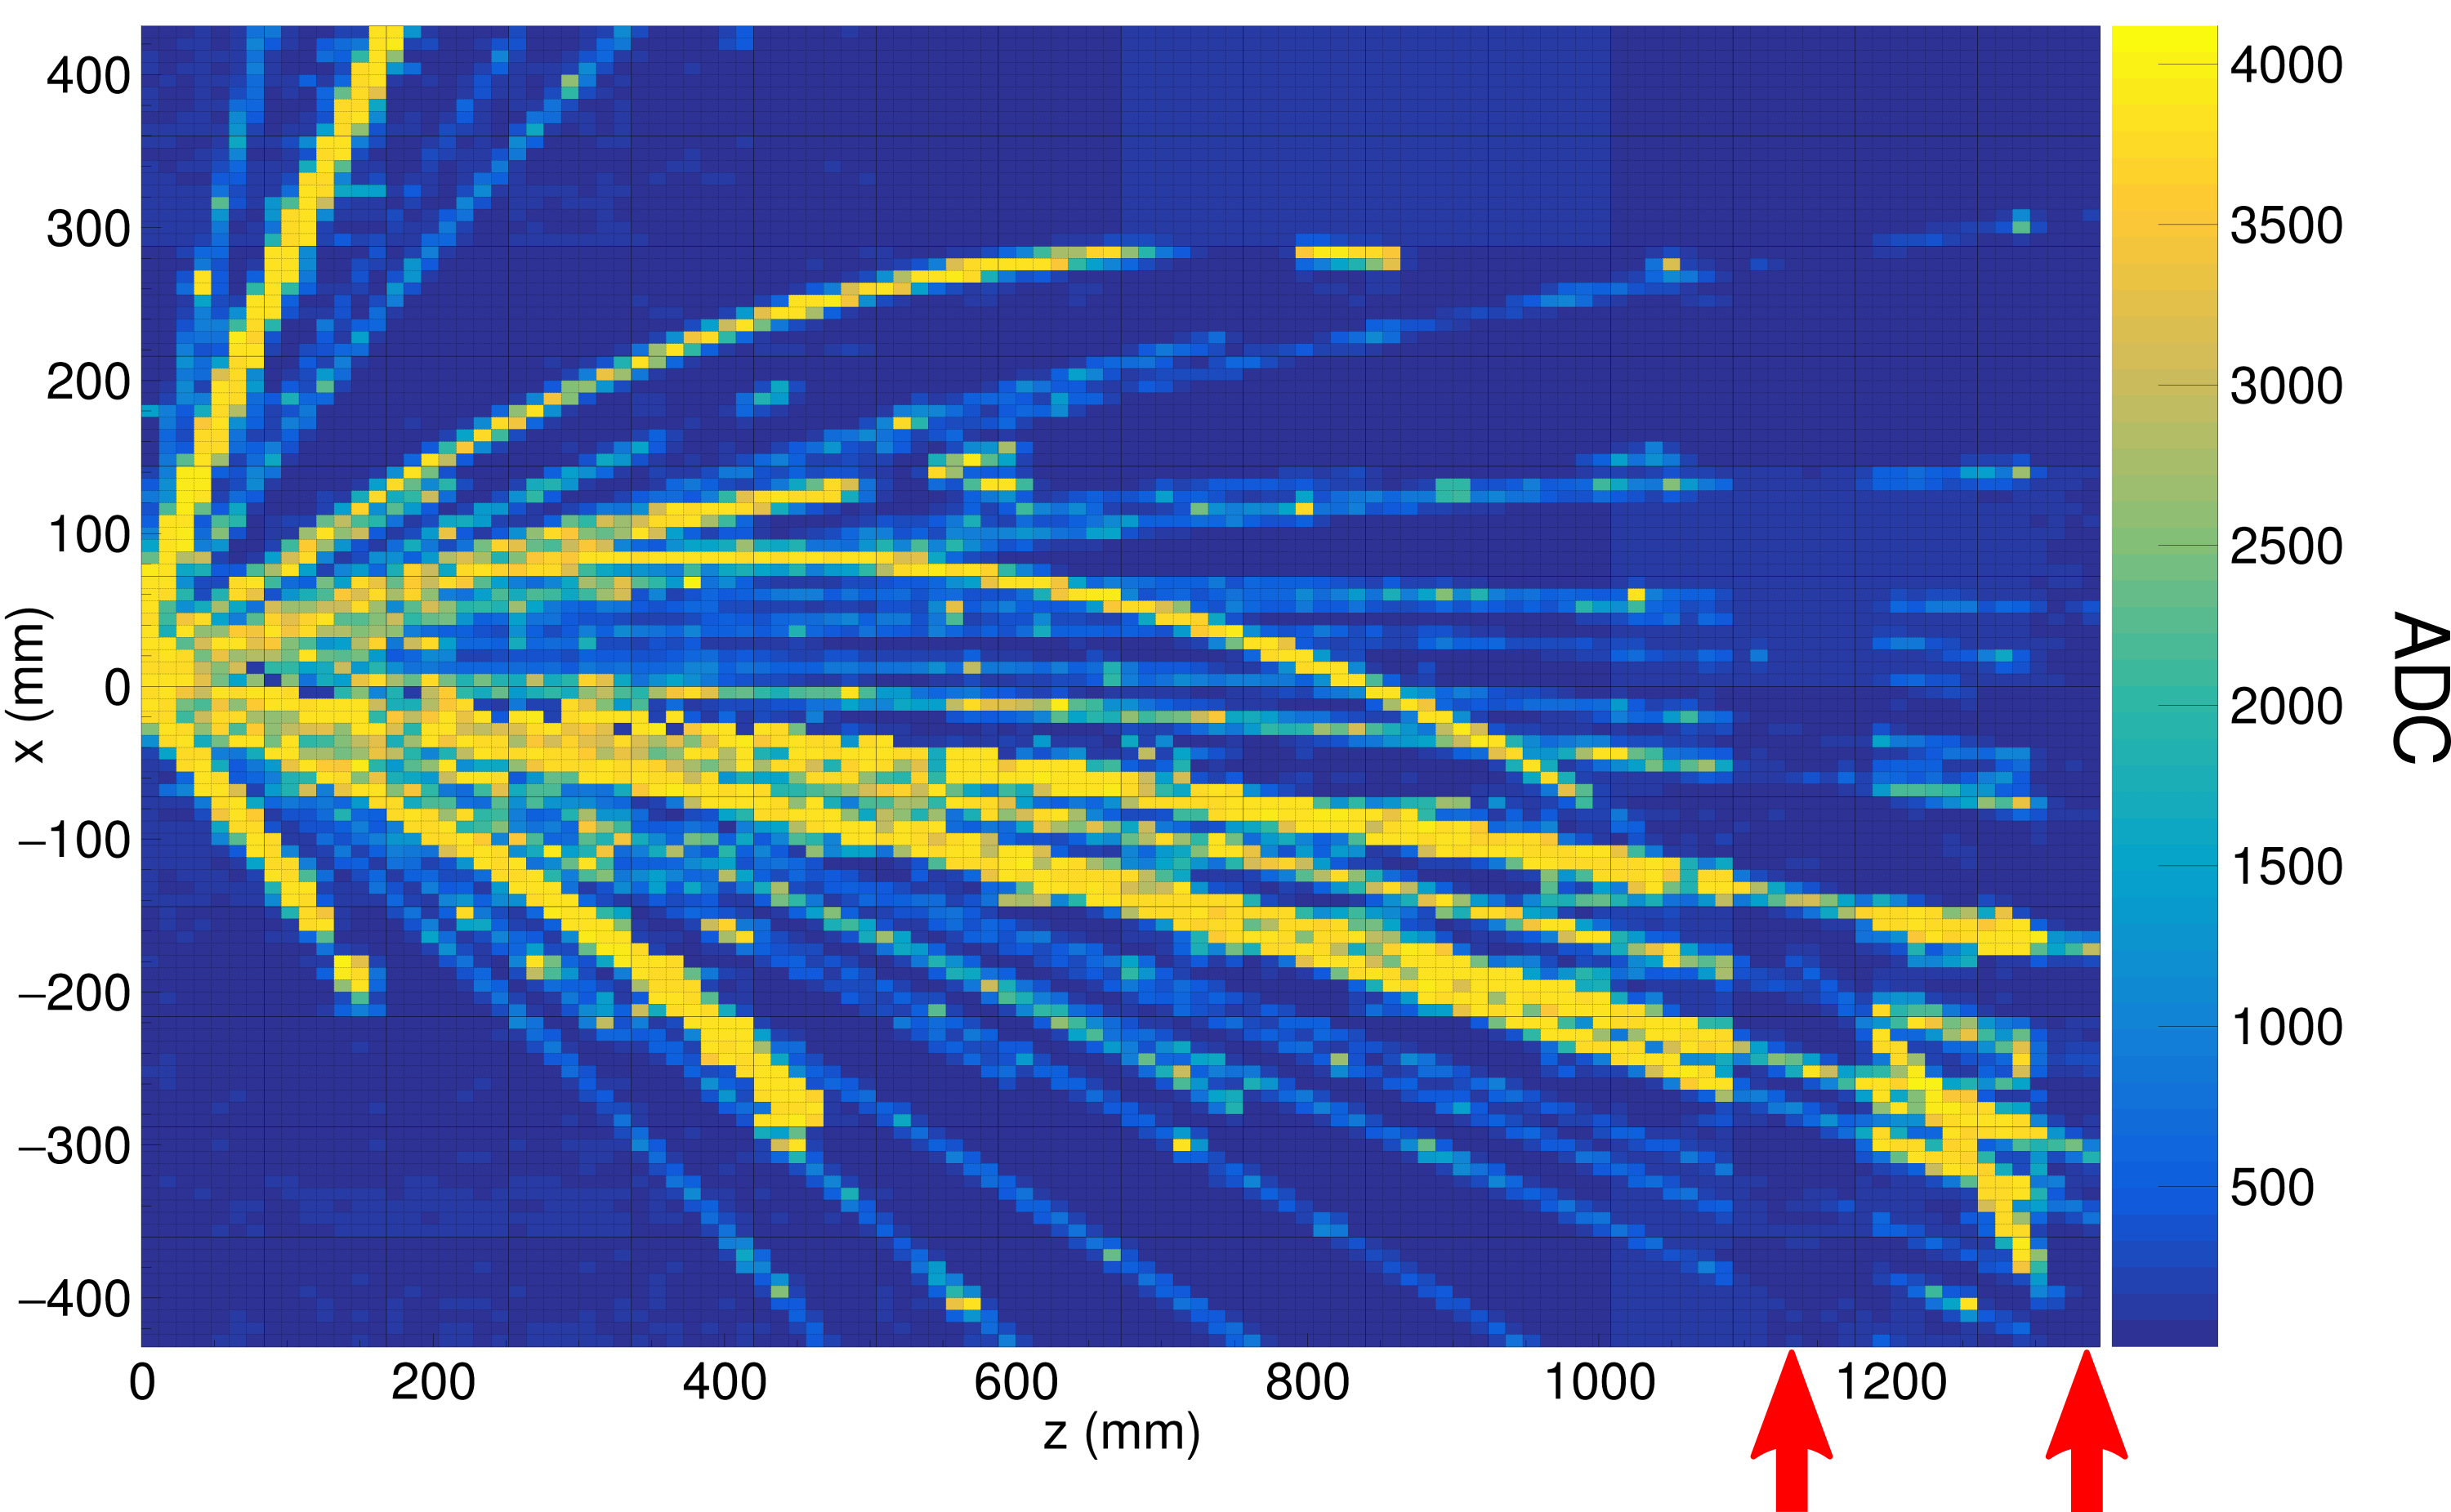
\includegraphics[width=\linewidth]{data.png}
\caption{Pad plane projection for a collision event in the TPC. Highlighted by red arrows are two regions of anode wires which had a reduced voltage of 1214 V. The voltage of the rest of the TPC anode wires are 1460 V. The reduction in voltage reduces the gain by a factor of about 10. }
\label{fig:data}
\end{figure}



Shown in Fig.~\ref{fig:cocktail} is a typical cocktail event, where one particle enters the TPC volume at a time and parallel to the pad plane, representing an ideal case for momentum and $dE/dx$ determination; as it does not suffer from inefficiencies of high multiplicity events seen in the collision experimental data. The primary goal of this data set was to calibrate the TPC in both momentum and dE/dx as will be discussed in Section~\ref{sec:cocktail}. 

\begin{figure}[!htb]
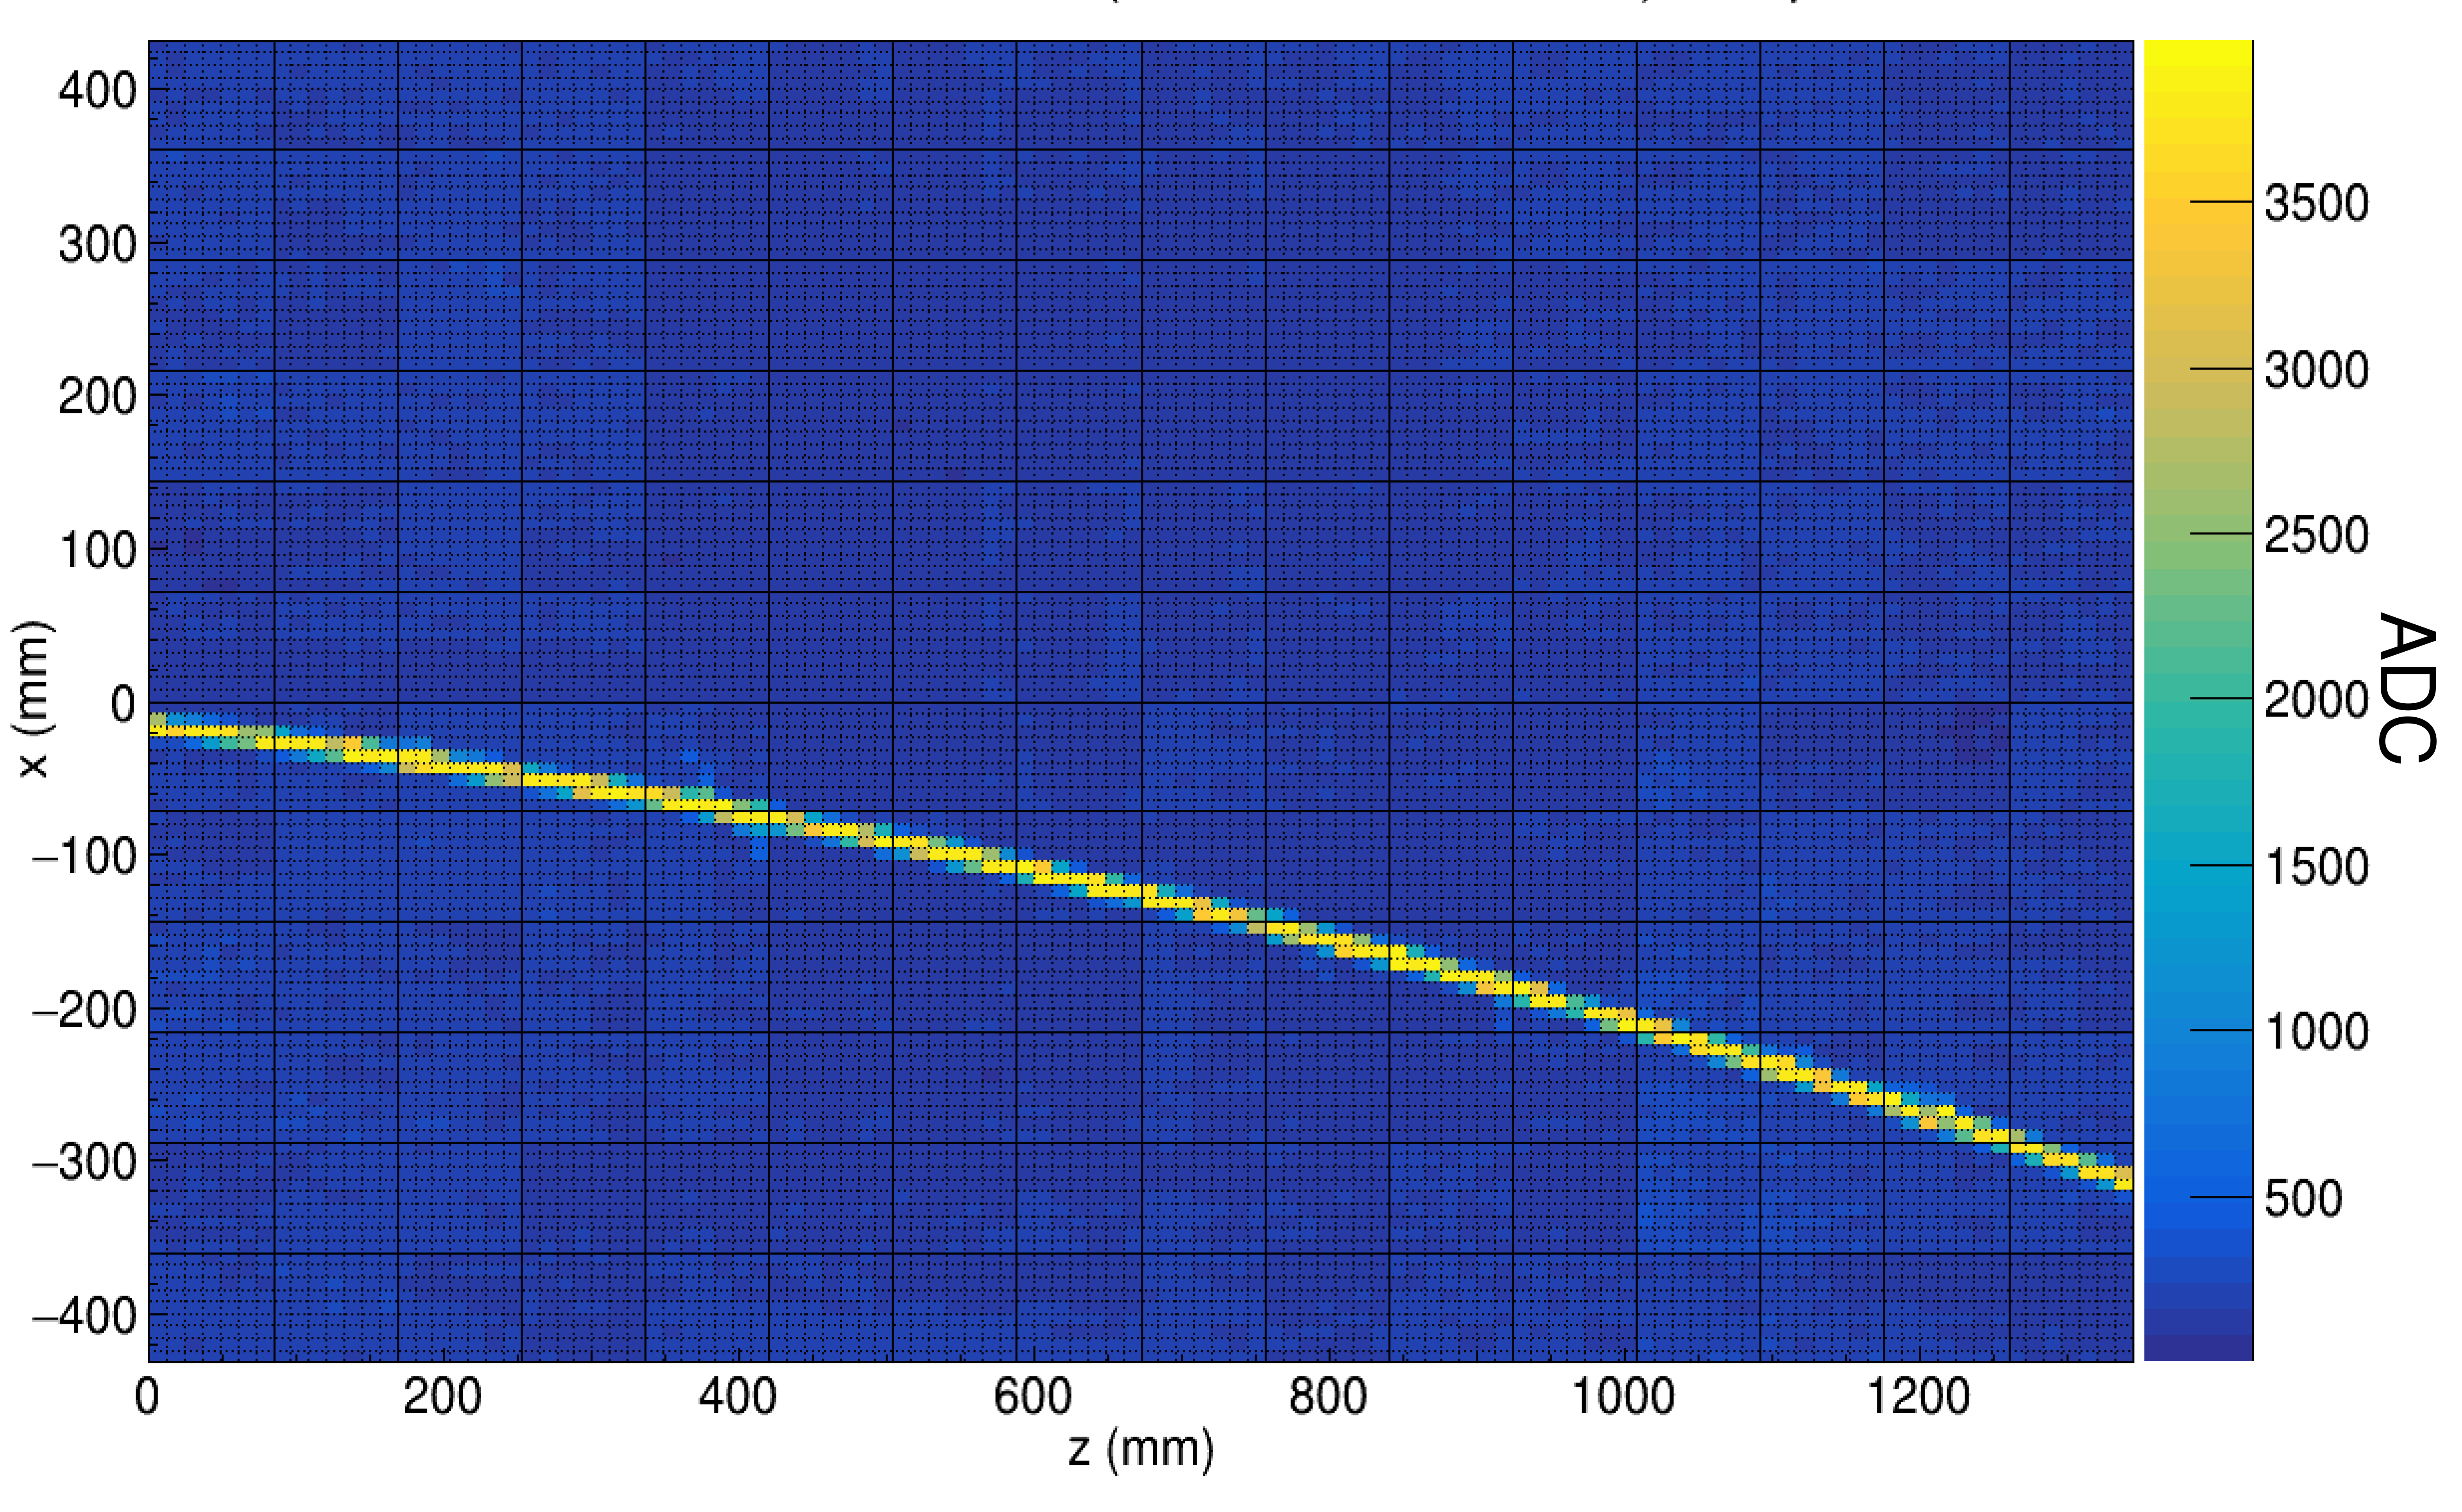
\includegraphics[width=\linewidth]{cocktail.png}
\caption{Pad plane projection for a cocktail event in the TPC.}
\label{fig:cocktail}
\end{figure}



\chapter{Data Analysis I: Calibration and Corrections}

Need to explain pedestal subtraction 
GG noise subtraction 

\section{Software}

The S$\pi$RITROOT software is modular tasked based code based on the FAIRROOT package written in C++ \cite{fairroot}. The main tasks in the S$\pi$RITROOT software reconstruction are:
\begin{itemize}
  \item Decoder task
  \item Pulse Shape Algorithm (PSA Task)
  \item Helix Track Finding Algorithm
  \item Clustering Algorithm
  \item Track Fitting (GENFIT package)
  \item Vertex Fitting (RAVE package)
\end{itemize}

The decoder task converts the binary data file into a container class which maps the electronics channels into the corresponding pads and (x,z) coordinates. 

There may be several pulses in a pad coming from two tracks passing under the same pad separated  by arrival time. Using an expected pulse shape the PSA task fits the signal pulses within a pad, giving the arrival time of the drifted electrons from each particular track. The height of the fitted pulse is proportional to the total charge of that event, Q and the y-coordinate is calculated as $y = v\cdot t_0$ where $v$ is the drift velocity and $t_0$ the arrival time. Combining the information from these first two tasks, (x,y,z,Q), we construct what is called a "hit". 

 The Helix Track Finding Algorithm finds the collection of hits belonging to one track out of all the hits in an event. The hits within a track are then reduced into clusters. A cluster's position is the average position of the hits within a cluster, with the total charge of the cluster being the sum of the hits charges. 
 
 A tracks average position is estimated by the cluster's average position. The clusters are then fitted in the GENFIT track fitting package \cite{genfit}, giving the final momentum of the track. A final vertex of the event is fitted from all tracks using the package RAVE \cite{rave}. 

\paragraph{Definition of clustering}

A brief description of the method of clustering is illustrated in Figure \ref{fig:topview}. It is impractical to cluster in both the x and z-axis and we only cluster the hits along one axis. The three clusters at the bottom of Figure \ref{fig:topview} are clustered along the x-axis and the upper three are along the z-axis, as shown by the bolded pads for one of the clusters in each direction.

 The clustering direction depends on the angle  of the track with respects to the x-axis, defined as $\theta$. For example, a track going along the z-axis the crossing angle is defined as $90^{\circ}$, and a track going along the x-axis defined as $0^{\circ}$. In the case that the crossing angle is $45^{\circ} < \theta \leq 90^{\circ} $ the clustering direction is along the x-axis. For $0^{\circ} < \theta \leq 45^{\circ}$ it is along the z-axis. 

 The position along the clustering direction is calculated by weighting the individual hit's positions by their charges $q_i$ and getting the mean value. The other direction is set to the center of the pad. For example if we are clustering along the x-axis for a cluster, the z-position is set to the center of the pad in the z-direction and vice versa. 

Clustering in this way gives us better position resolution for calculating the position of each cluster. You could imagine if we calculated the clusters only along the x-axis for tracks with $\theta \approx 0^{\circ}$ the x-position is not well defined. By clustering in the direction most perpendicular to the track, we get a better position resolution.

\begin{figure}[H]
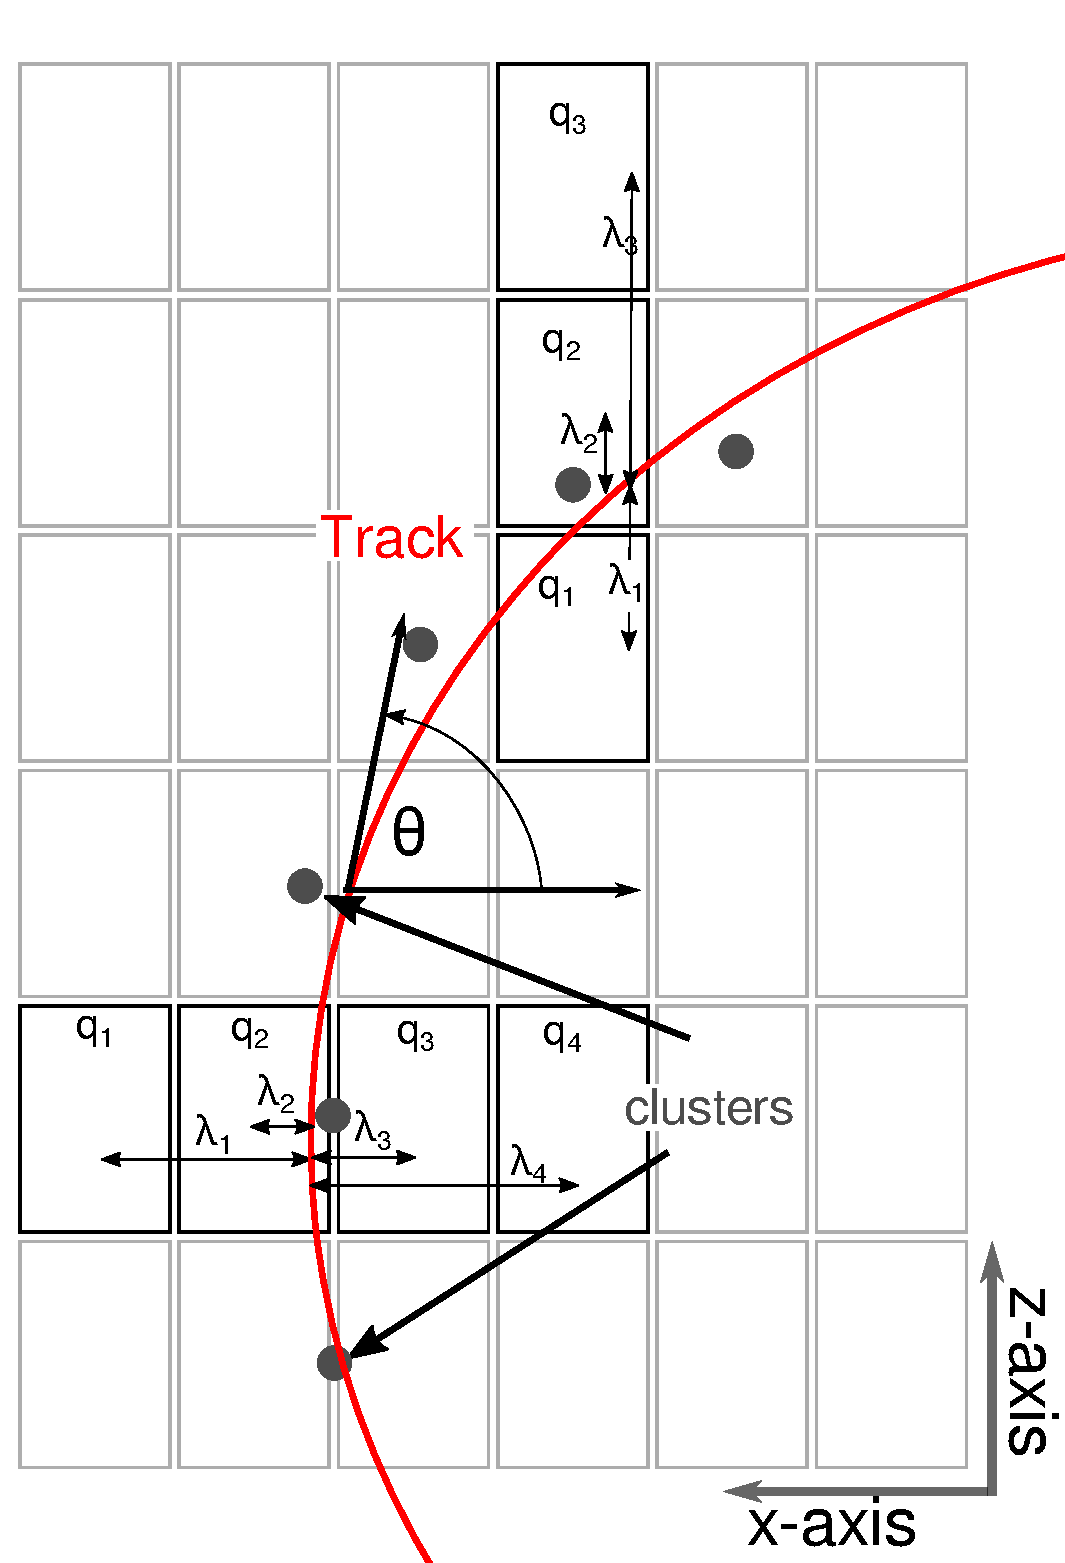
\includegraphics[scale=.5]{top_view_helix_ext.pdf}
\caption{Cartoon graphic of a top down view of a fit to a track passing through several pads. The bolded pads and the charges $q_i$ represent the hits belonging to that pad and the clusters of the track representing the average position of the track. The three clusters at the bottom are clustered in the x-direction and for the upper three clustered in the z-direction. The estimate of the position of the avalanche is given by the track fit and the position from the center to each pad to the $\bar{x}$ position is given as $\lambda_i$.}
\label{fig:topview}
\end{figure}

\begin{figure}[H]
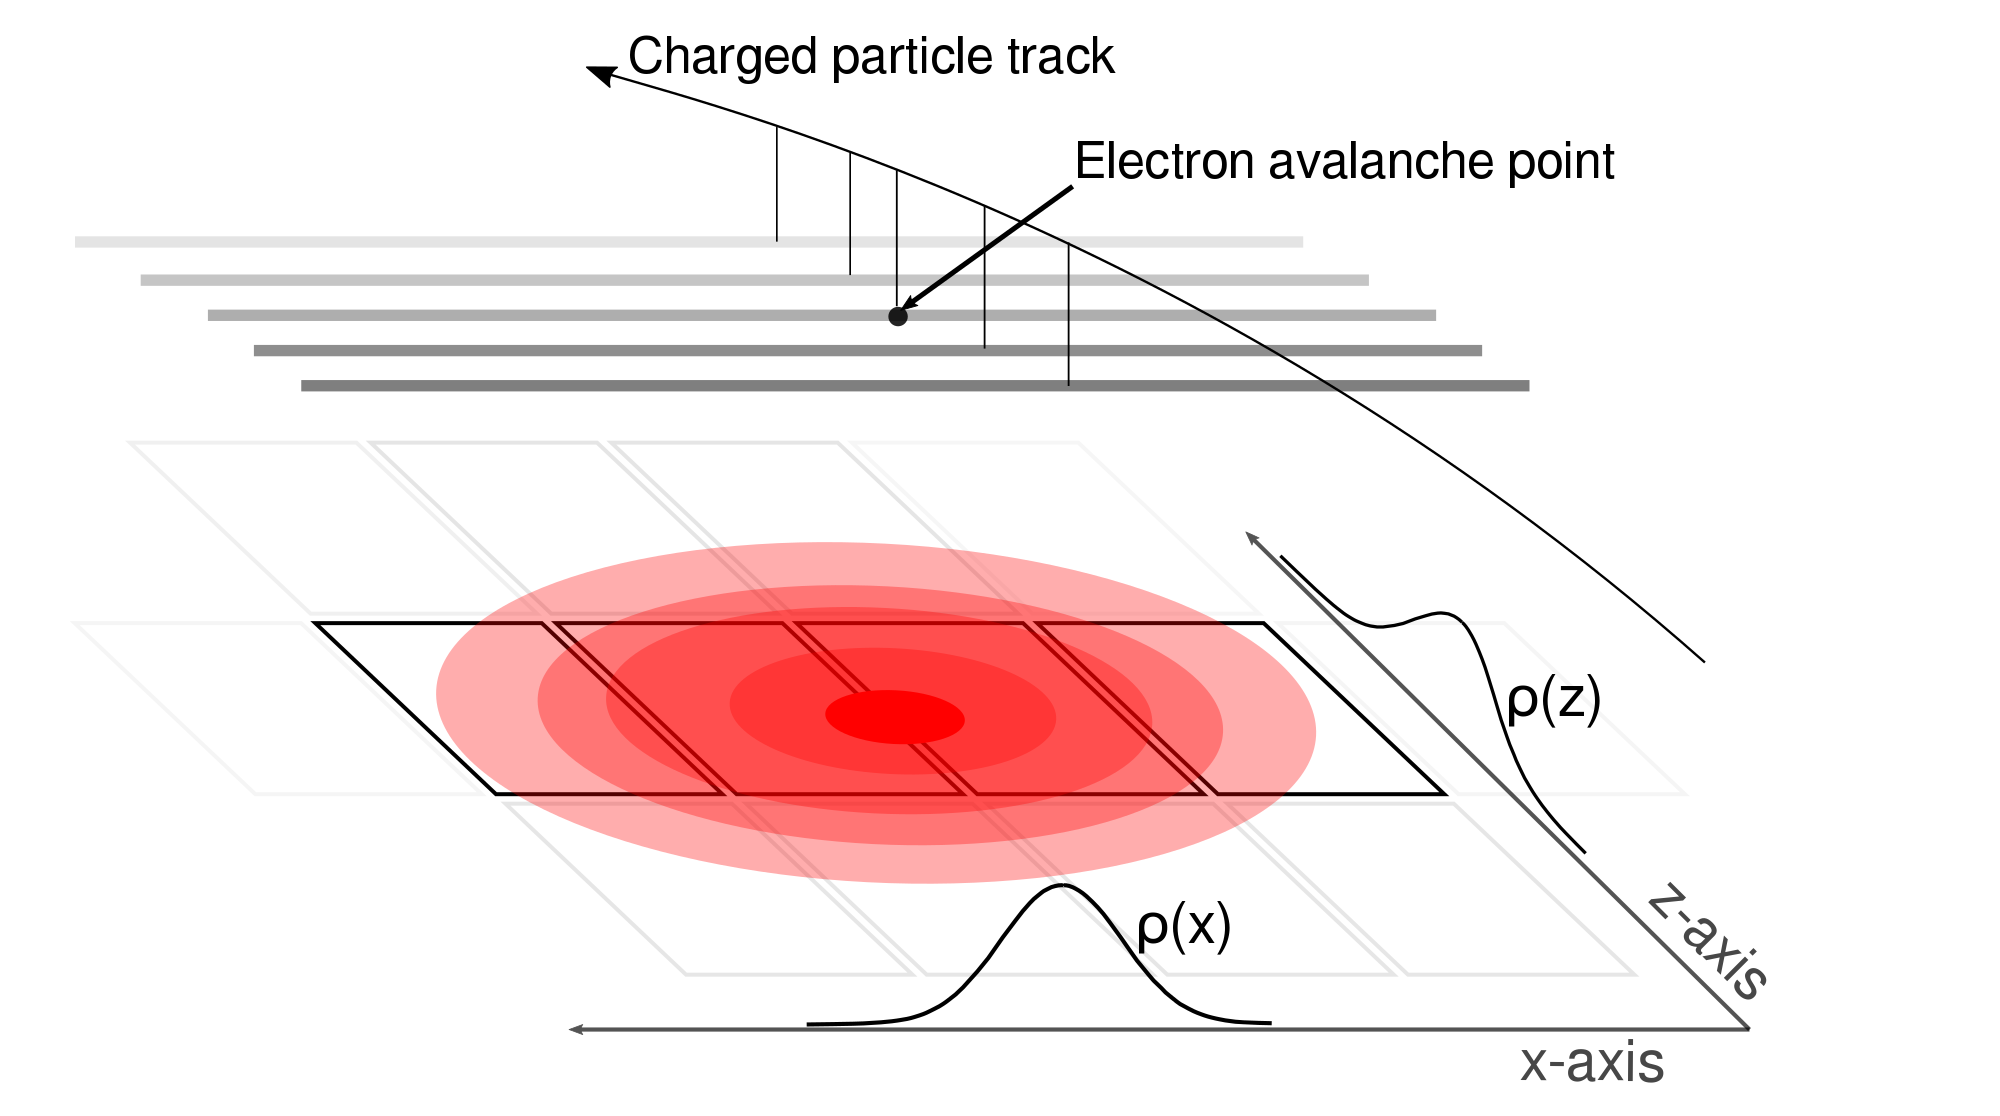
\includegraphics[width=\linewidth]{padsat_Large}
\caption{A cartoon illustration of the charge distribution resulting from an electron avalanche on one wire and the projections of the distribution onto the two axis $\rho(x)$ onto the x-axis and $\rho(z)$ onto the z-axis. The orientation of the wire planes is flipped upside down to display the perspective better.}
\label{fig:prf}
\end{figure}



\section{Calibrations and Corrections}


\subsection{Cocktail calibration}

\begin{table*}\centering
\ra{1.3}
\begin{tabular}{@{}rrrrcrrrcrrr@{}}\toprule
& \multicolumn{3}{c}{$100 MeV$} & \multicolumn{3}{c}{$100 MeV$} & \multicolumn{3}{c}{$300 MeV$}\\
\cmidrule{2-4} \cmidrule{6-8} \cmidrule{10-12}
& &\multicolumn{2}{c}{Measured} & & \multicolumn{2}{c}{Measured} & & \multicolumn{2}{c}{Measured}\\
\cmidrule{3-4} \cmidrule{7-8} \cmidrule{11-12}
Particle &\phantom{abc} & Raw & E$\times$B\\
\midrule
p   & 882.8 & d & d & 903.5 & e & e &\phantom{abcdef} & f & f \\
d   & 817.1 & d & d & 898.5 & e & e & 1621.1 & f & f\\
t   & 589.5 & d & d & 887 & e & e & 1612.4 & f & f  \\
$^{3}$He  & 1617.3  & d & d & 1795.2 & e & e & 3236.4 & f & f\\
$^{4}$He  & 1405.6  & d & d & 1782.9 & e & e & 3226.4 & f & f \\
\bottomrule
\end{tabular}
\caption{Summary of expected cocktail. }
\label{tb:cocktailsummary}
\end{table*}

Cocktail Calibration 
Picture of cocktail before and after ExB effect
Table of LISE++ expected cocktail energies ridigity setting of dipole magnets (reference big rips line)



\subsection{Electronics calibration}
Pulse the ground grid. 
\begin{figure}[H]
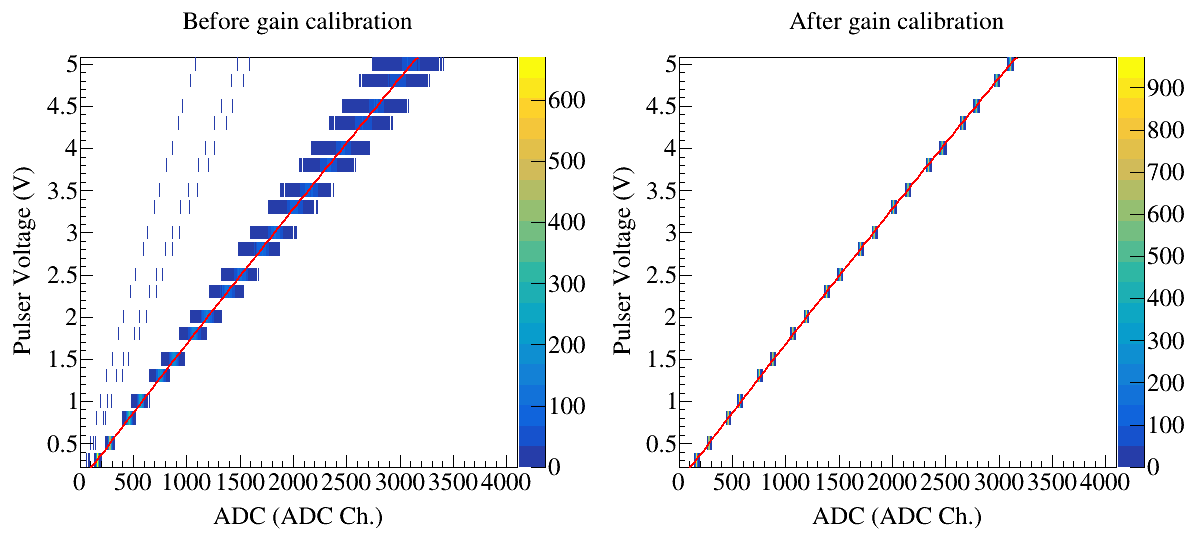
\includegraphics[width=\linewidth]{gaincalib.png}
\caption{Calibration of electronics}
\label{fig:gaincalib}
\end{figure}

\subsection{Anode gain calibration}

\begin{figure}[H]
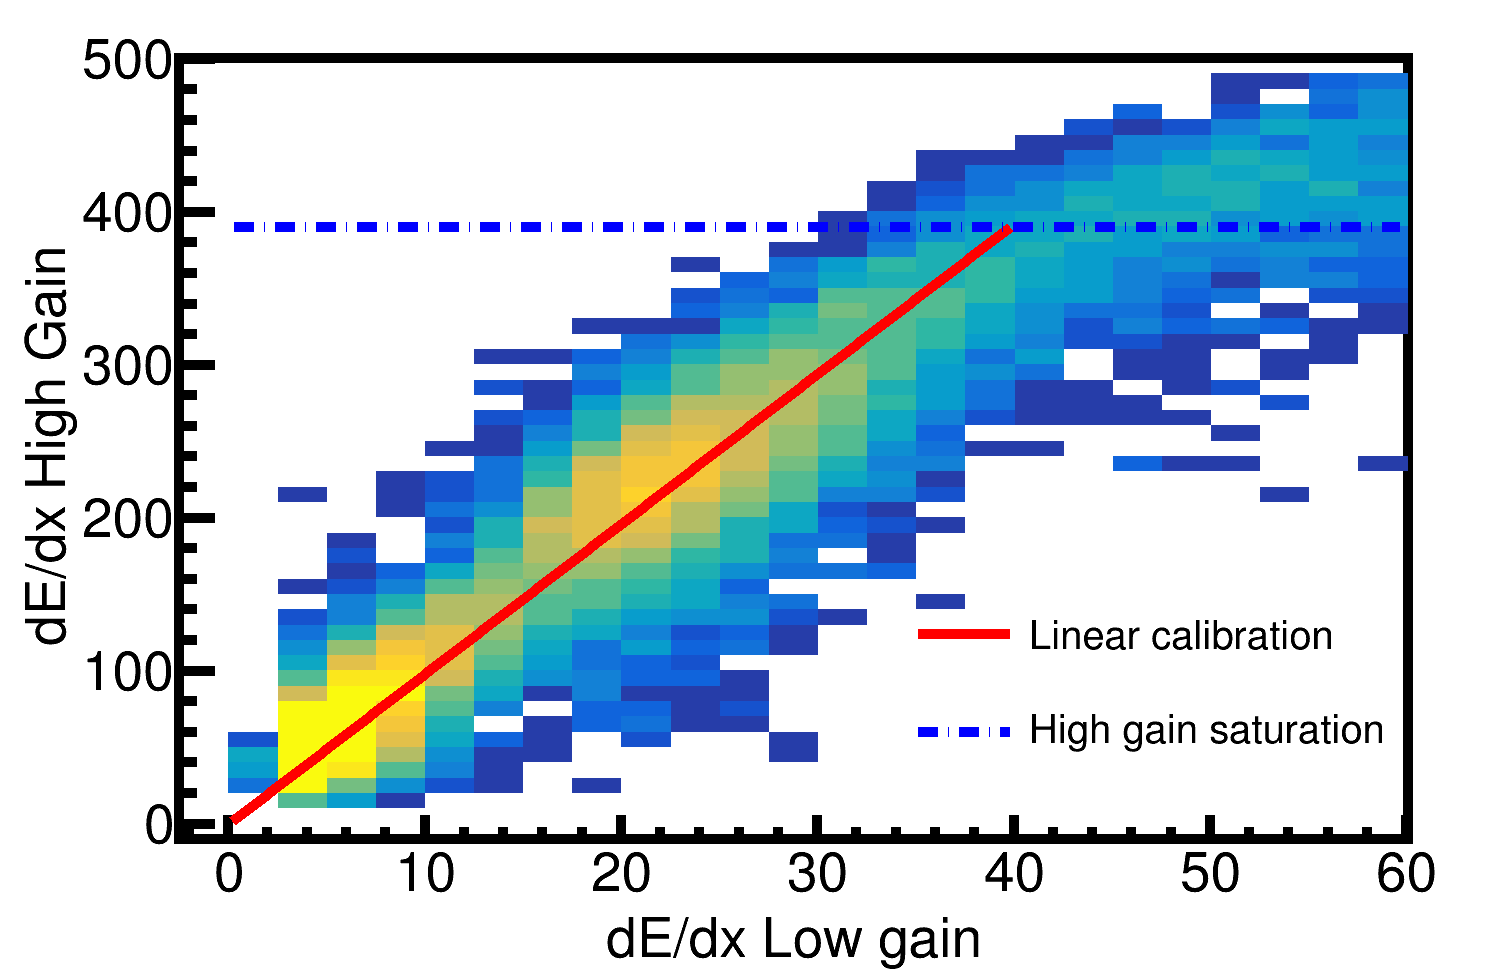
\includegraphics[width=\linewidth]{highlowcal.png}
\caption{Calibration of low high.}
\label{fig:highlowcal}
\end{figure}

Picture of low vs high gain channels and fit

\subsection{Extending the dynamic range of the Electronics}
Add paper here. 

\subsection{Space Charge Corrections}
Overview
Discuss the relevant time scales, drift lengths, magnitudes, and locations of space charge

\begin{figure}[H]
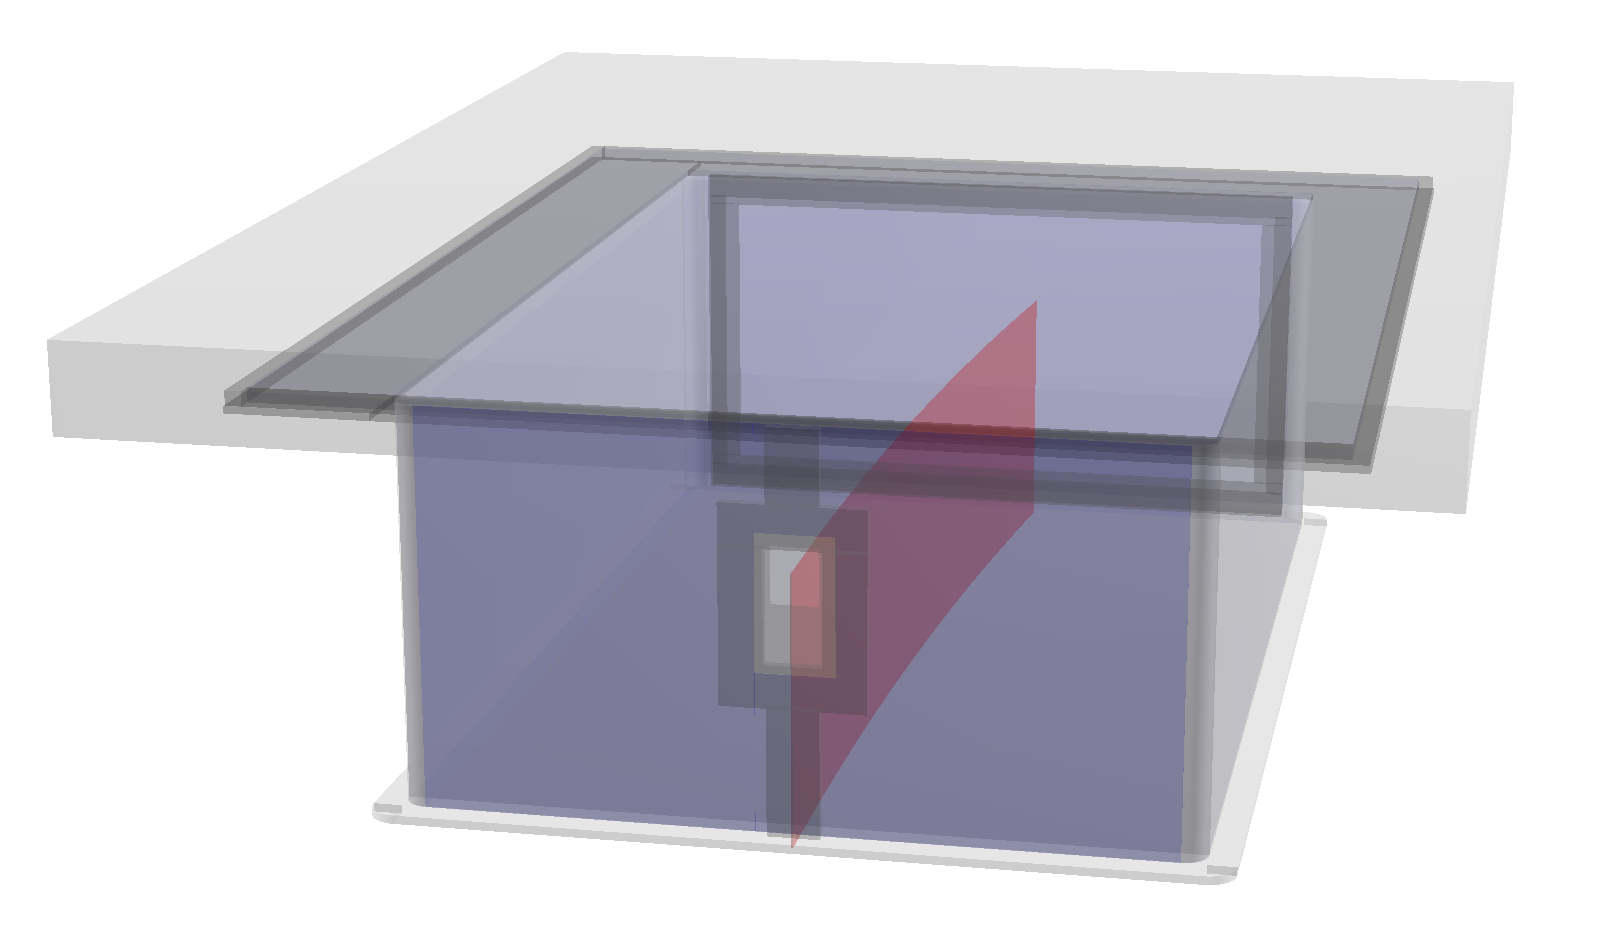
\includegraphics[width=\linewidth]{spacechg_cartoon.png}
\caption{Location of space charge in 132 Sn}
\label{fig:spacechg_cartoon}
\end{figure}

\begin{figure}[H]
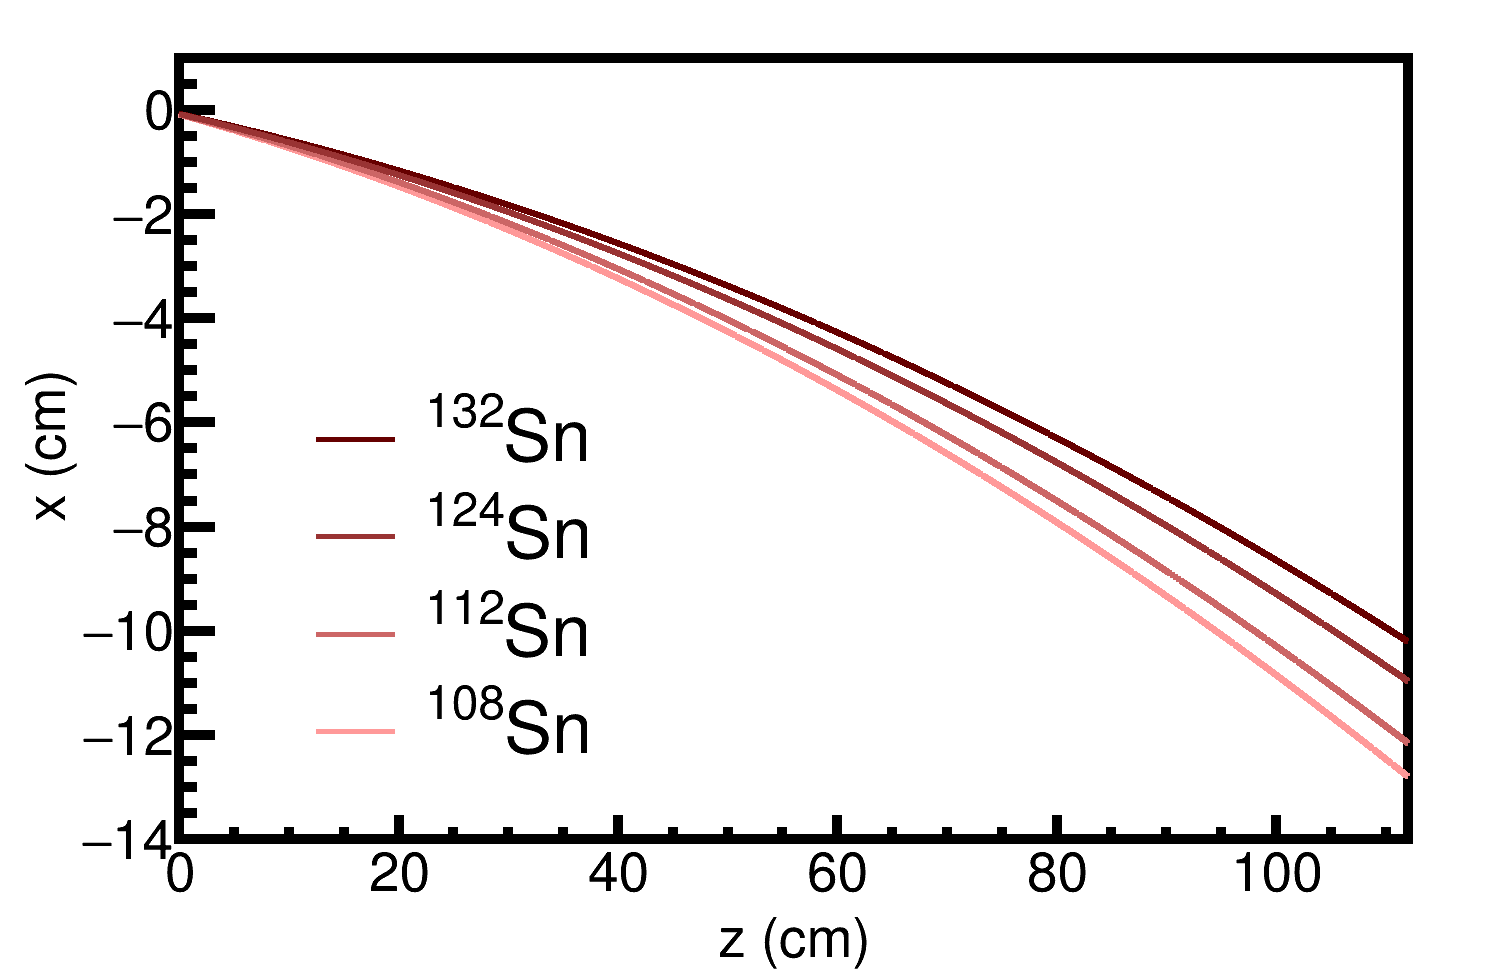
\includegraphics[width=\linewidth]{beampath.png}
\caption{Beam path of the experiments}
\label{fig:beampaths}
\end{figure}


\begin{table}[!htp] % not just 'h!'
\centering % not a center environment
\begin{tabular}{
  @{}
  l
  S[table-format=1.2]
  S[table-format=1.2]
  S[table-format=1.2]
  S[table-format=5.2]
  S[table-format=5.2]
  @{}
}
\toprule
Beam Energy Loss  &
 {${}^{132}$Sn} &
 {${}^{124}$Sn} &
 {${}^{112}$Sn} &
 {${}^{108}$Sn} &
  {Avg.}\\
  
\midrule
$\si{\kilo\eV\per\centi\meter}$ & 11.2   &.034  &5.43   &  903   &150     \\
\bottomrule
\end{tabular}

\caption{Average energy loss of each beam.}
\label{tb:beameloss}
\end{table}

Reference appendix for poisson solver 
Tables for ion drift velocity in P-10 Gas reference Sauli
Figure of sDAC or POCA 
Figure of cartoon of what is happening to tracks
Figure of correction map in TPC and MC map 
Figure of before and after correction BDC vs reco momentum
Figure of track residuals before and after?


In theory, a TPC functions with the electric and magnetic fields parallel to each other. In this way the electrons move opposite to the electric field winding tightly around the magnetic field lines, reducing transverse diffusion in the process. In practice, due to the finite size of the dipole magnet and field cage, there are traverse components to both the electric and magnetic fields. These transverse components introduce drift velocities in the transverse directions, causing a shift in the measured cluster positions of the track. Thereby introducing systematic shifts in the calculation of the momentum and the vertex calculation. 

Most of the time the beam does not undergo a nuclear collision with the target and passes through the TPC drift volume. The KATANA array threshold was set to veto such events, ensuring the gating grid remain closed to prevent the large amount of charge deposited by the beam into the avalanche region. While the electron drift velocity is fast enough for the electrons produced by the unreacted beam to terminate on the closed gating grid, the drift velocities of the positive ions produced are of order $10^{-4}$ times slower. At higher beam rates the positive charge is allowed to pile up producing a region of positive space charge, introducing perturbations to the nominal electric field. 

Since the beam comes in along the z-axis, and the drift direction of the ions is in the -y direction, we can estimate the charge density as an uniform sheet charge. The surface charge density is related to the beam rate, ion drift length, ion drift velocity, and the energy loss of the beam. Though the incoming beam comes randomly, the slow drift velocity combined with the high beam rate makes the uniform approximation valid. Tracking or estimating the beam rate as a function of time with in a given run would provide a better estimate of the space charge. Or experimentally a laser system could be pulsed after each event (throughout the drift volume), giving the experimental correction map for the drift. While the potential for a laser system was implemented in the field cage design, a laser system ultimately was not developed for the \spirit tpc. 

The beam rate within a run is roughly constant, therefore we can estimate the space charge and provide a first order correction for the space charge effect. 

As mentioned in CHAPTER ???, the cocktail beam momentum was well known to within 1\% as set by the BIGRips spectrometer. Also time of flight analysis of upstream and downstream scintilators also independently confirmed the beam rigidity setting. The expected momentum is given in TABLE ??? as calculated by from the beam rigidity setting of the magnet (WHICH MAGNET). The measured momenta as determined by the TPC software (given in FIG TABLE ), shows a disagreement on the level of 5\% too high. We noticed that if one only uses the first 90 layers (out of 112) of the TPC, the momenta is lower; one should expect the momentum to go higher as the track length is shorter (short tracks effectively are straight lines). 
In the cocktail beam there is no un-reacted beam causing any significant space charge. The magnetic field map of the SAMURAI magnet has been calculated by TOSCA simulation CITE ???, and several points have been verified experimentally with a hall probe to be within XXX \%. We assume that the electric field (to first order) is uniform in the y-direction. Using Garfield++ CITE ???, we can model the transverse drift of the electrons in the presence of such fields. 

A grid of electrons uniformly distributed in the TPC model space were drifted to the gating grid position. The final shifts in the x and z positions was measured. 


\section{Monte Carlo Simulation}
We use Geant4 as and event generator for performing Monte Carlo Simulations in the TPC. A scale model of field cage, front window, front window frame, pad plane, and aluminum top plate are modeled. The correct materials are used as well as the field cage is modeled with P-10 gas at a density of ????. By using Geant4 we can also input the the magnetic field map of the SAMURAI dipole magnet (as calculated by the SAMURAI group via a TOSCA simulation).  In this way any particle type may be studied and the full interactions (scattering, decay, energy loss, path taken, etc.), are accounted for. The output of this simulation is a series of energy loss points which contain the amount of energy lost in $keV/cm$ and the position in $(x,y,z)$.

Separate software tasks model the converting energy loss into electrons, the drifting of electrons, the avalanche process, and the electronics response.

\begin{figure}
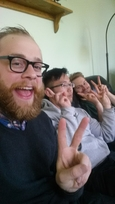
\includegraphics[scale=.01]{place}
\caption{A summary of all the effects modeled in the TPC MC simulation.}
\label{fig:place}
\end{figure}

\subsection{Drift Task}
The drift task takes the energy loss points calculated from Geant4 and converts them into electrons.  and then modeling their drift behavior in the field cage. As discussed previously the various processes[CITE To formula about drifting electronc]


 A full microscopic treatment of the stochastic nature of each electron would be too cumbersome; most of the properties of the electrons are described by macroscopic quantities can be described by 
The charge of each MC point is converted to the total number of electrons liberated in the P-10 gas. This is a well understood property of proportional counters and is stable over a wide range of velocities and particle types [CITE BOOK]. The conversion factor of P-10 can be calculated by considering the partial volumes of each component of the gas.  \ref{eq:kev2el}.

\begin{equation}
Number of e^{-} = 28 keV/cm
\label{eq:kev2el}
\end{equation}

\subsection{Pad Response Task}
After the avalanche process of the previous task, the total charge of the event is split over several pads defined by the Pad Response Function (as discussed in section ????). As shown in Fig.~\ref{fig:onepad}, there are three wires that lie directly above a given pad. The $z$ coordinate of the avalanche can only be one of these three wires, where as the $x$ coordinate can be any value along the wire. The functional form of the software PRF (given in Eq.~\ref{eq:softPRF}), was tuned to match the experimental data. Shown in Fig.~\ref{fig:mcdataPRF}, we see the tuned software PRF can match the experimental PRF from data over several crossing angles (as mentioned in Chapter ???? governs the shape of the PRF). 

\begin{equation}
PRF(x,z) = \frac{1}{2\pi\sigma_z\sigma_x}\exp^{\frac{-{(x-x_o)}^2}{2\sigma_x^2}}\exp^{\frac{-{(z-z_o)}^2}{2\sigma_z^2}}
\label{eq:softPRF}
\end{equation}

\begin{figure}
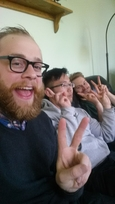
\includegraphics[scale=.005]{place}
\caption{A cartoon of the wires over one pad. }
\label{fig:onepad}
\end{figure}

\begin{figure}
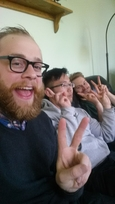
\includegraphics[scale=.005]{place}
\caption{Comparison of MC and data PRF}
\label{fig:mcdataPRF}
\end{figure}

\subsection{Electronics Task}
The electronics task takes the total charge on each pad and simulates the electronics response, converting electronics into ADC channels. Accounting for the pedestal, the measured output in ADC channels (for a given gain setting) is given in Eq.~\ref{eq:etoADC}.

\begin{equation}
\mathrm{1 ADC }= \frac{ADC_{\mathrm{Max}} - ADC_{\mathrm{Pedestal}}}{G*f_c}
\label{eq:etoADC}
\end{equation}

\subsection{Simulating Saturation}
Add figure showing saturated time bucket spectra with location of saturation identified and with pulse shape from embedding I would like to add and how it blocks it.
Add Figure with 2D pad plane response with and without saturation flag


\section{Monte Carlo Track Embedding}
Add Figure of MC track embedding 



Track embedding is the process of taking a simulated MC track from Geant4 and embedding its response into a real data event. After reconstructing this new embedded event we match the input MC track embedded to its corresponding final reconstructed track.  By doing so we can evaluate the response of the entire TPC system to any given input value. The TPC system is composed of three major components (each which can introduce errors and or biases) the software, the detector, and the experimental setup.  

As discussed in [SOFTWARE CHAPTER] the software is composed of several task, each which introduce some error. Table {REF TABLE] listing some of the errors each task may introduce illustrating how difficult propagating the errors would be through each system. 

The detector system itself introduces errors related to the physical processes of the measurement itself. To address this we model the TPC (and its materials) in a Geant4 simulation which provides an accurate description of various interactions of a particle traversing the materials (including the gas volume) of the TPC. 


 software is the most straight forward; let the software routine process an input and measure the result. Understanding the measurement requires modeling the physics involved in the theory and operations of TPC's and the  electronics. The experimental setup itself is quite large and complex, several ancillary detectors such as the Kyoto multiplicity array, Krakow veto array, Active veto array, beam identification detectors, etc. Even if a full accurate model could be constructed the complex trigger logic of the DAQ system would be impossible to model. If we notice that the biases and errors of the entire experimental setup is contained in the measured experimental data. Therefore, by inputting the MC data into a real experimental event (and measuring the output of that MC track) we can estimate the errors of the experimental setup. 

The software analysis routine and the bias introduced by the trigger settings of the experiment introduce systematic errors in the reconstruction of tracks

\subsection{MC and Data Comparison}
Add Figure of Pad response function for pion,proton.... for MC vs Data vs angles...
Add Figure of Number of clusters of MC vs Data
Add Figure of dEdx MC vs Data
Add Figure of Momentum resolution MC vs Data
Add Figure of track residuals? MC vs data?


\section{Efficiency Corrections}
Add Figures of efficiency vs angles in TPC polar angle plot for pions


Since the \spirit TPC is a fixed target experiment it's angular coverage is certainly not 4$\pi$. Because the target is several cm away from the widow of the field cage the geometric acceptance is not even 2$\pi$. The rectangular design complicates the calculation of the geometric acceptance, or the efficiency.

\section{Beam Particle Identification}
Figures of beam contaminants in our beam PID line. 
Table of beam purity reference to Jon's thesis paper

\section{Solid angle coverage}
\chapter{Data Analysis II}

\section{Radio Isotope Beam Factory (RIBF) Facility }
\label{sec:beam}
%Cyclotron facility overview.
%Samurai line overview.
%Beam line element overview.
%Big rips beam PID. reference 
The primary and secondary beams were produced at the Radioactive Isotope Beam Factory (RIFB) facility at RIKEN, in Wako-shi, Japan. The RIBF facility starts with two primary beam types, ${}^{132}$Xe and ${}^{238}$U, which are produced by an ion-source and accelerated to progressively higher kinetic energies by 1 linear accelerator (RILAC), and 4 different cyclotrons (RRC, fRC, IRC, and SRC), until they reach a beam energy of \SI{345}{\MeVA}. Figure~\ref{fig:samuraiBeamLine} shows the later stages of the cyclotrons and the following beam lines they feed into.

\begin{figure}[!htb]
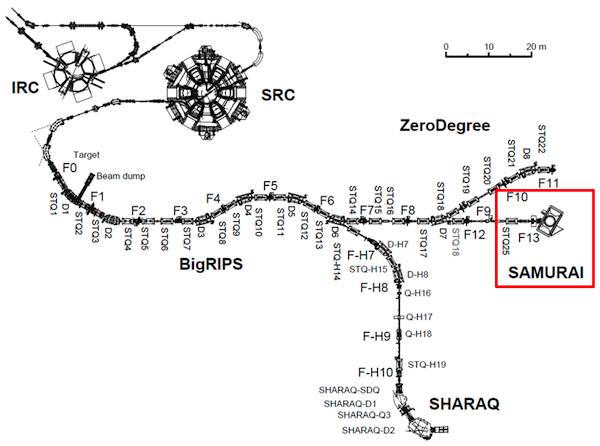
\includegraphics[width=\linewidth]{SAMURAI-beamline.png}
\caption{Overview of the RIBF, BigRIPS, and SAMURAI beamline.}
\label{fig:samuraiBeamLine}
\end{figure}

After the SCR, the primary beams impinge on a rotating \SI{3}{\milli\metre} Be target which produces many different species by fragmentation. These fragments are then separated by the BigRIPS spectrometer which is tuned to the particular secondary fragment of interest. This is accomplished through several dipole magnets, slits, and wedge degraders. The resulting secondary beam is not pure and the purity depends on the capability of BigRIPS to deliver the secondary beam of choice and the primary beam used. 

In these set of experiments several beams were produced with varying intensities and purities. Table~\ref{tb:beams} summarizes the average qualities of the 4 secondary beams produced in the two experimental campaigns where most beams were delivered with an intensity of \SI{10}{\kilo\hertz}. 

 \begin{table*}\centering
\ra{1.3}
\begin{tabular}{@{}ccccc@{}}\toprule 
 Primary Beam & Secondary Beam & Energy at mid target \si{\MeVA} & Intensity \si{\kilo\hertz} & Purity (\%) \\ [0.5ex] 
 \midrule
 ${}^{238}$U   & ${}^{132}$Sn   &  269.2  &  9.5  &  54   \\
 ${}^{238}$U   & ${}^{124}$Sn   &  270.3  &  9.1  &  10  \\
 ${}^{124}$Xe  & ${}^{112}$Sn   &  270.4  &  7.6  &  48  \\
 ${}^{124}$Xe  & ${}^{108}$Sn   &  269.3  &  7.5  &  52   \\
 \bottomrule
\end{tabular}
\caption{Primary and secondary beam properties produced in the \spirit TPC experimental campaigns. }
\label{tb:beams}
\end{table*}


\section{Beam Particle Identification}


\begin{figure}[!htb]
\centering
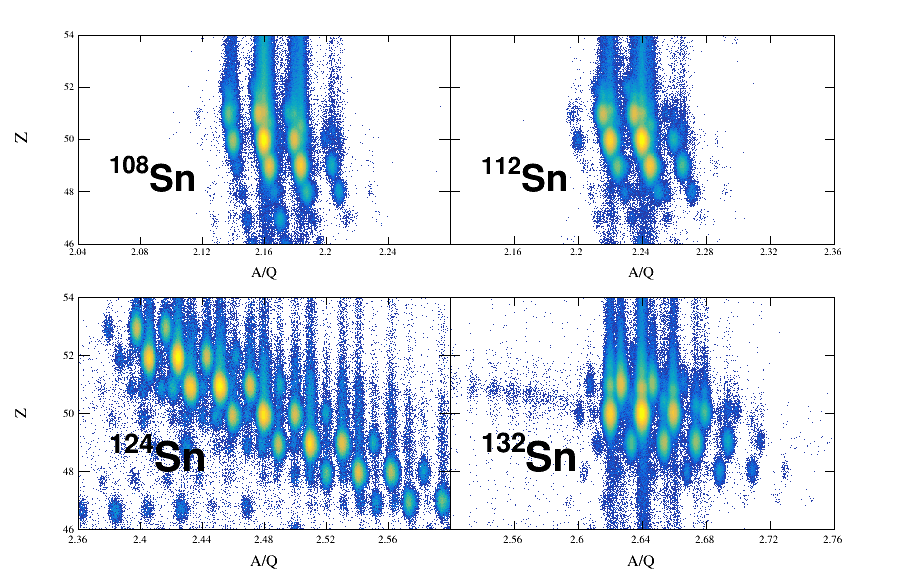
\includegraphics[width=\textwidth]{beamPID.png}
\label{fig:beampid}
\caption{Overall beam PID for all the systems. Several contaminants other than the desired secondary beam can be seen.}
\end{figure}


\begin{figure}[!htb]

     \centering
     \begin{subfigure}[b]{0.49\textwidth}
         \centering
         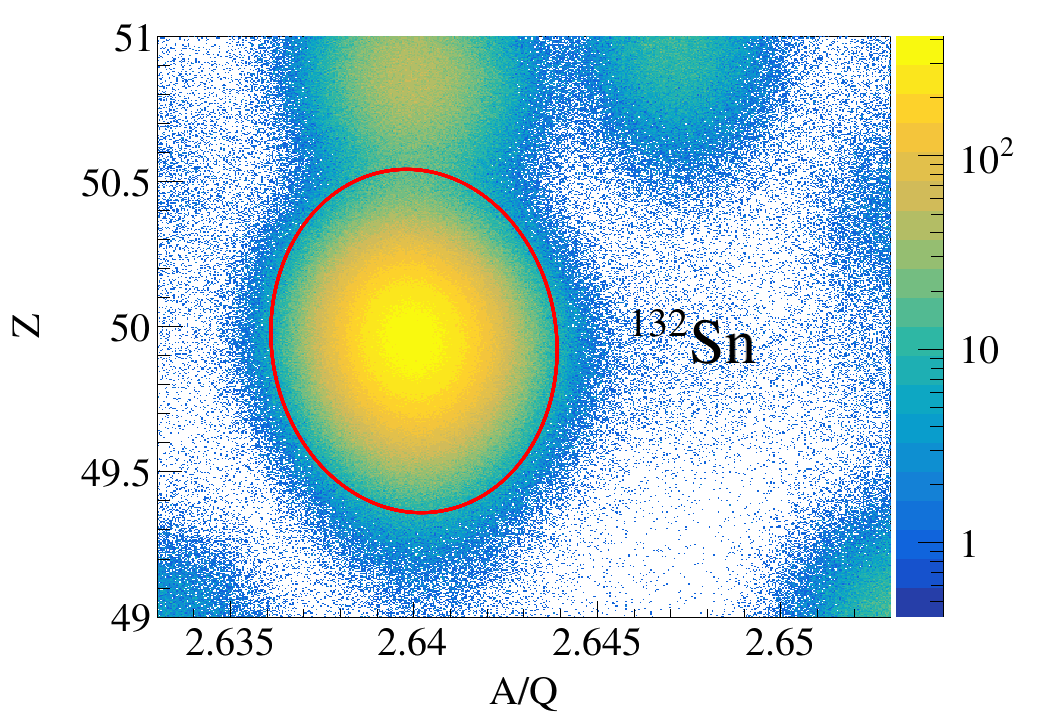
\includegraphics[width=\textwidth]{beam-Sn132.png}
         \caption{$\tin{132}{124}$ Beam particle identification.}
         \label{fig:beampid132}
     \end{subfigure}
     \hfill
     \begin{subfigure}[b]{0.49\textwidth}
         \centering
         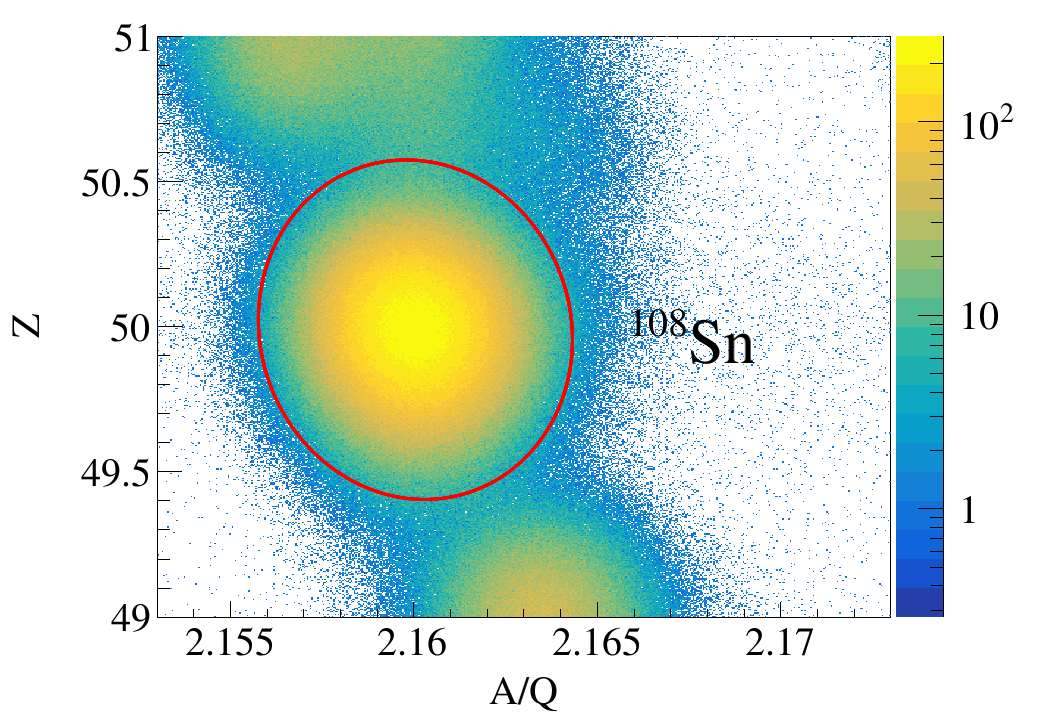
\includegraphics[width=\textwidth]{beam-Sn108.png}
         \caption{$\tin{132}{124}$ $\pi^-$ angular spectra.}
         \label{fig:beampid108}
     \end{subfigure}
        \caption{$\tin{108}{112}$ Beam particle identification. }
        \label{fig:beampidTwo}

\end{figure}


%Figures of beam contaminants in our beam PID line. 
%Table of beam purity reference to Jon's thesis paper
The secondary beam is produced through the projectile fragmentation of the primary beam off of a \SI{3}{\milli\metre} thick, rotating Be target \cite{inflightsep}. The resulting fragments are filtered in-flight to the desired seconary beam. The in-flight separation is handled by the BigRIPS fragment separator which is shown in Fig.~\ref{fig:samuraiBeamLine}. The dipole magnets D1 and D2 act as a velocity filter, selecting on certain magnetic rigidities $\beta\rho$. Several sets of slits further purify the secondary beam quality by throwing away particles which do not focus on the right focal planes. These are the areas where the particles with different velocities focus to different locations in space, which occur at F3,F5, and F7 positions.  Each beam is tracked with the remaining part of the BigRIPS spectrometer tracking system. The particle identification of each beam is achived by the TOF-B$\rho$-$\Delta$E method described in \cite{bigrips}, where the Time of Flight (TOF) information is given by the time it takes to cross two plastic scintilators at F3 and F7 focal planes, and the $\Delta$E information is given by the MUlti-Sampling Ionization Chamber (MUSIC) \cite{music}. From this method the atomic charge, Z, and mass to charge ratio, A/Q, of each particle was measured and separate species represent two-dimensional Gaussians in this space. 

Figure~\ref{fig:beampid} shows the beam PID for all the systems for events which satisfied the trigger, several contaminants other than the desired secondary beams still passed through the BigRIPS spectrometer and made it into the TPC. The beam purity of each desired secondary beam is listed in Table~\ref{tb:beams}. The desired secondary beam of interest can be selected by using an appropriate gate around the corresponding group, since the BigRIPS PID resolution is good enough to separate separate beam types. Each particle gate is selected by fitting a multivariate normal distribution with two variables defined as,

\begin{equation}
  f(x,y)=\frac1{2\pi\sigma_x\sigma_y\sqrt{1-\rho^2}}\exp\left\{
  \frac{-(x - \mu_{x})^2/\sigma_x^2-(y-\mu_{y})^2/\sigma_y^2+2\rho
  xy/\sigma_x\sigma_y}{2(1-\rho^2)}\right\},
   \label{multiGauss}
\end{equation}
where x=A/Q, y=Z, $\mu$ is the mean values, and $\sigma$ are the Gaussian widths of the two variables. The gates drawn in Fig.~\ref{fig:beampidTwo} are summarized in Table~\ref{beamParameters}. 

\begin{table}[!htb]
  \begin{center}
    \begin{tabular}{cccccc}
      \hline 
      Particle Type & $\mu_\mathrm{A/Q}$ & $\sigma_\mathrm{A/Q}$ & $\mu_\mathrm{Z}$ &
      $\sigma_\mathrm{Z}$ & $\rho$\\
      \hline\hline 
      ${}^{132}$Sn & 2.64 & 0.0014 & 49.95 & 0.209 & -0.052 \\
    %  $\tin{124}{112}$ & 2.24005 & 0.00150934 & 49.9906 & 0.194804 & -0.0671999 \\
    %  $\tin{112}{124}$ & 2.47995 & 0.00182327 & 49.961 & 0.214745 & -0.0742297 \\
      ${}^{108}$Sn & 2.16 & 0.0015 & 49.99 & 0.207 & -0.059 \\
      \hline
    \end{tabular}
    \caption{Multivariate normal distribution fit parameters for four beams.
    \label{beamParameters}}
  \end{center}
\end{table}
Figure~\ref{fig:beampid132} shows a zoomed in view of the PID centered around the ${}^{132}$Sn beam and Fig.~\ref{fig:beampid108} the ${}^{108}$Sn beam. The red lines represent the cut where particles identified inside the circle represent the beam events which are identified as the good beam events. For both ${}^{132}$Sn an ${}^{108}$Sn a 2.83$\sigma$ cut is taken around the mean values.  


\section{Edge Cuts}

\begin{figure}[!htb]

    \centering
    \begin{subfigure}[t]{0.45\textwidth}
        \centering
        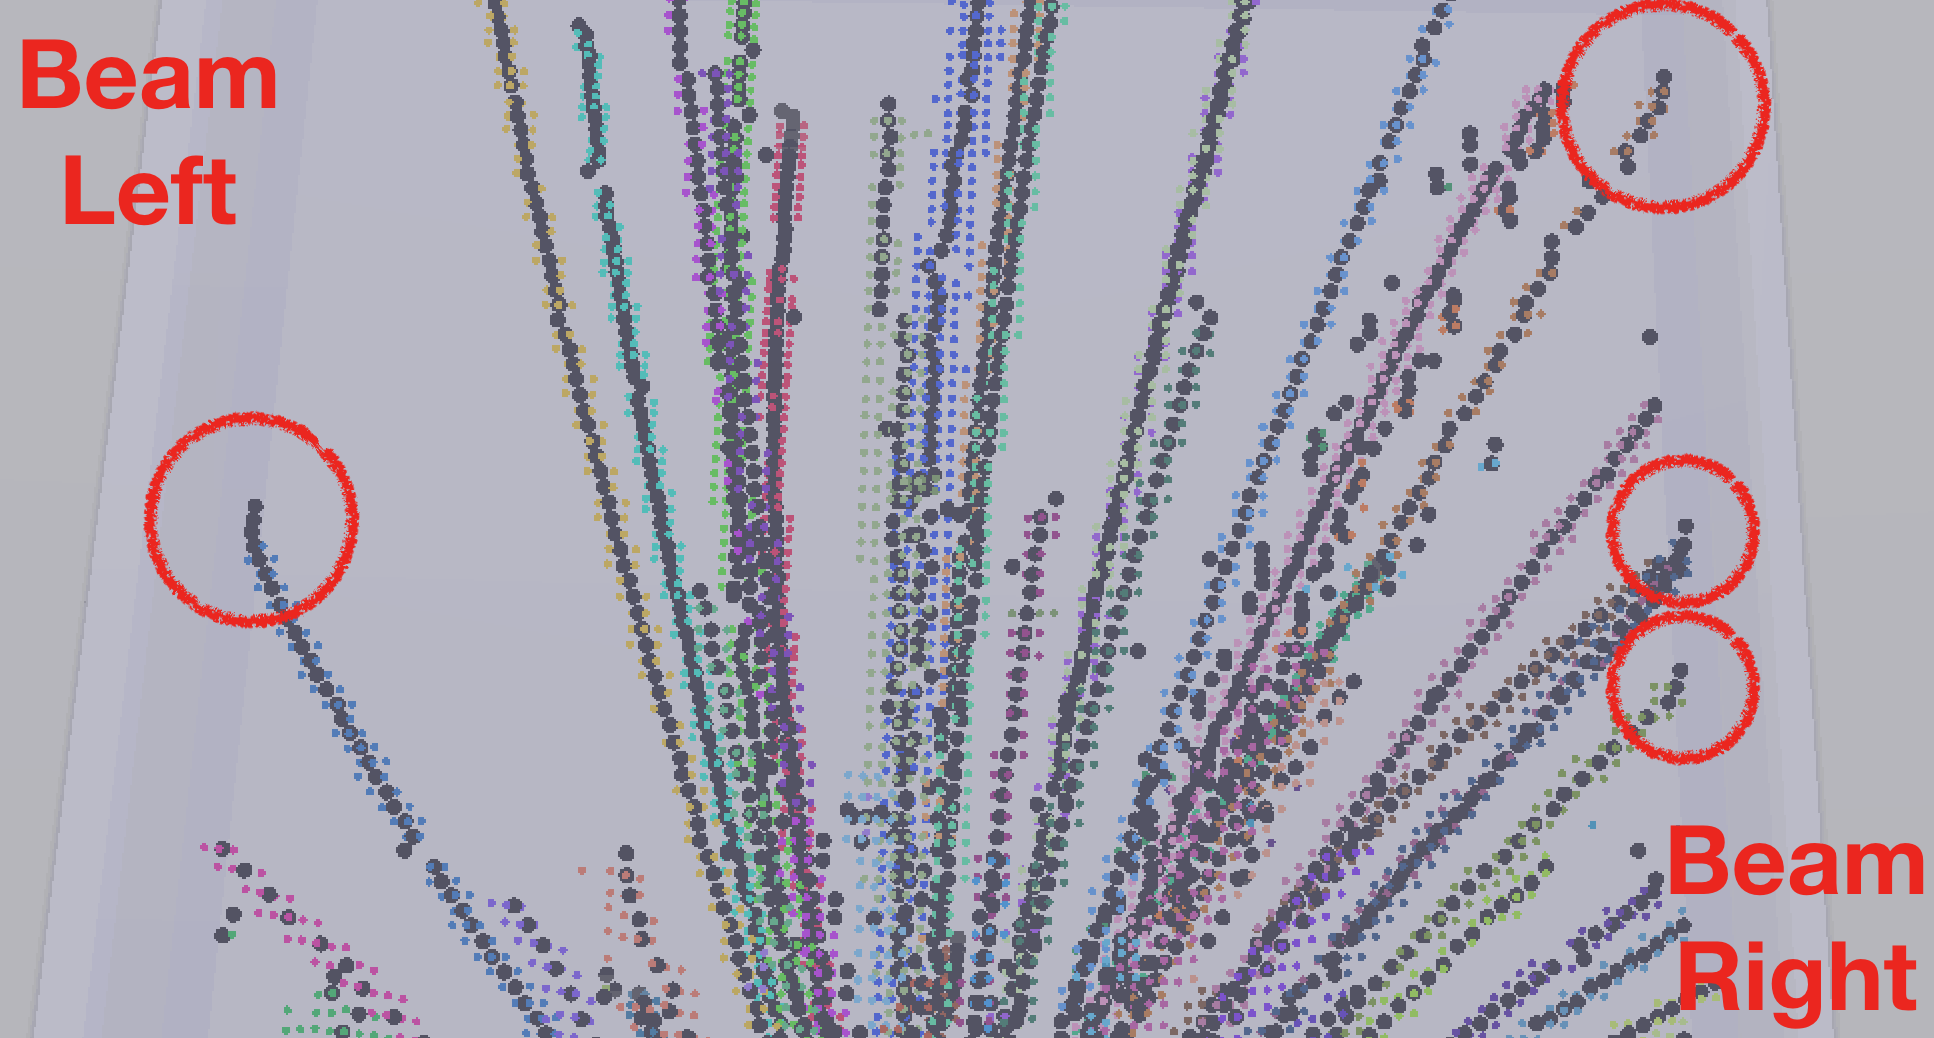
\includegraphics[width=\linewidth]{clusterLR.png} 
        \caption{Top view of the tracks showing the edge effect on the left and right sides of the TPC.} 	   \label{fig:clusterLR}
    \end{subfigure}
    \hfill
    \begin{subfigure}[t]{0.45\textwidth}
        \centering
        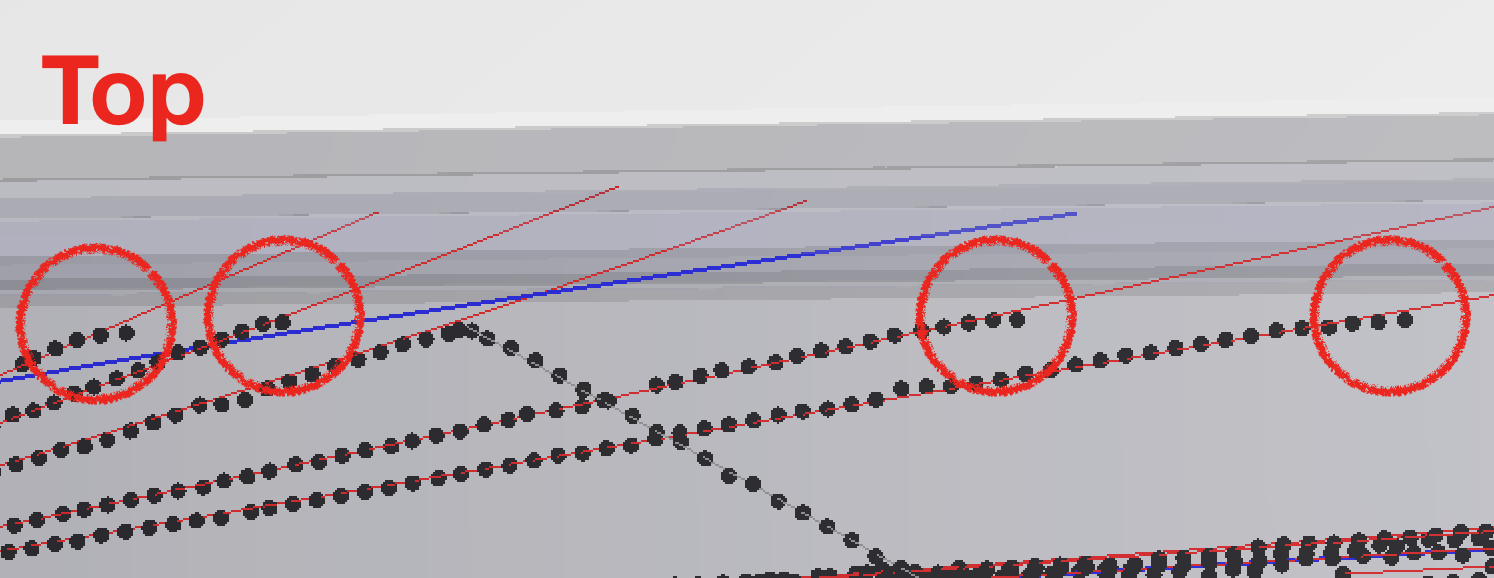
\includegraphics[width=\linewidth]{clusterTop.png} 
        \caption{Side view of the TPC showing the edge effect near the top.} \label{fig:clusterTop}
    \end{subfigure}
    
    \begin{subfigure}[t]{0.45\textwidth}
        \centering
        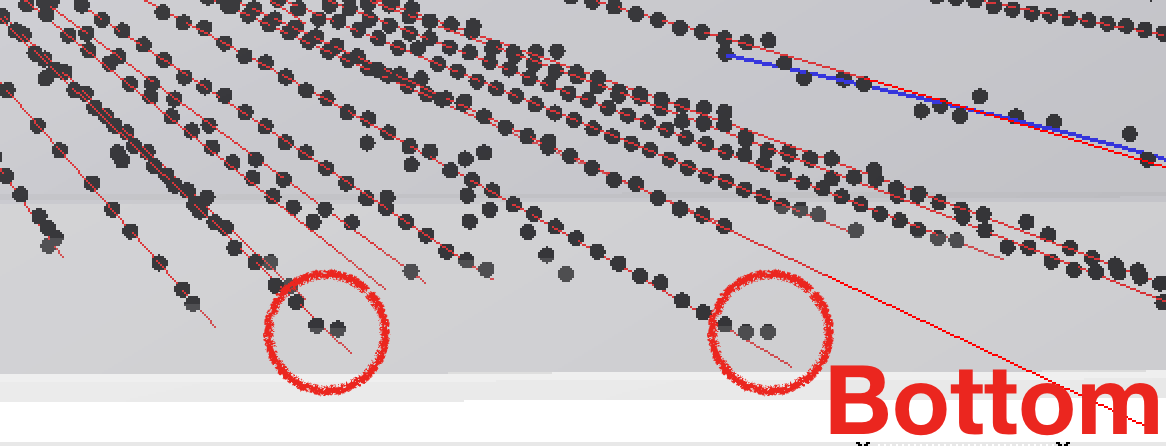
\includegraphics[width=\linewidth]{clusterBottom.png} 
        \caption{Side view of the TPC showing the edge effect near the bottom.} \label{fig:clusterBottom}
    \end{subfigure}
\caption{}    
\label{fig:edge}
\end{figure}

Near the edges of the detection volume, the clusters of tracks significantly deviate from the trend of the fitted track as seen in different view of the reconstructed clusters in Fig.~\ref{fig:edge}.  This effect comes from an edge effects where the last pads on the edges of the pad-plane have no neighboring pads containing charge, and therefore the last pad, or in the case of the vertical time bucket spectrum, represents the last known position of the collected charge. In this case the cluster position is biased towards the inside of the TPC. While the number of affected clusters is small as compared with the total number in the track, but the deviation at the end of the track is enough to start causing issues in the momentum reconstruction. Simple cuts were taken to graphically remove these clusters around the left,right, top, and bottom of the TPC. The hits that were cut out satisfied the following conditions, 

\begin{equation*}
  |x|\geq420~\mathrm{mm},\quad y\leq-522+\mathrm{y_o}~\mathrm{mm},
  \quad\mathrm{and}\quad y\geq-64+\mathrm{(Hit\ Shift)}~\mathrm{mm}.
\label{eq:hitshift}
\end{equation*}



\section{High Density Cut}


\begin{figure}[!htb]

     \centering
     \begin{subfigure}[b]{0.49\textwidth}
         \centering
         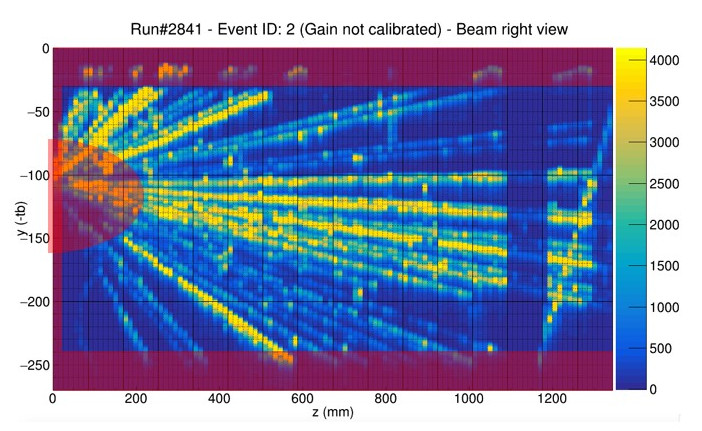
\includegraphics[width=\textwidth]{sideviewHighDenCut.jpg}
         \caption{Side view.}
         \label{fig:sideHigh}
     \end{subfigure}
     \hfill
     \begin{subfigure}[b]{0.49\textwidth}
         \centering
         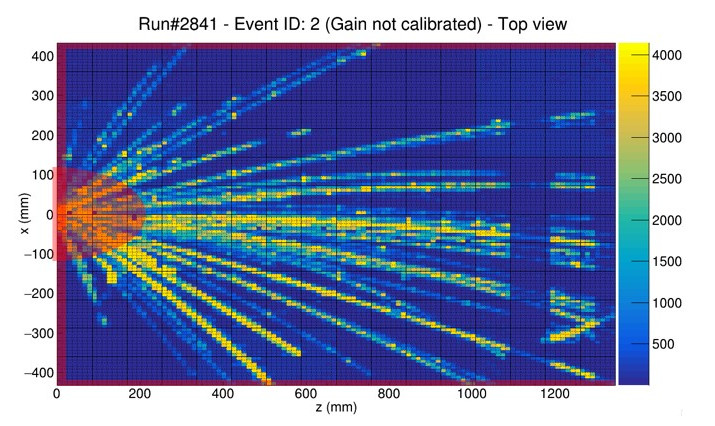
\includegraphics[width=\textwidth]{topviewHighDenCut.jpg}
         \caption{Top view.}
         \label{fig:topHigh}
     \end{subfigure}
        \label{fig:highcut}
        \caption{Views showing the high density and edge cuts.}
        \label{fig:elipsecut}
\end{figure}
The track multiplicity in each event is quite high and since the tracks all originate from a common vertex, the density of tracks near the target region is very high. In this region the track separation is too small for the software to correctly determine and sort the charge information into the appropriate track. The information provided by extra vertex point from external BDC tracking described in \ref{sec:bdc}, provides all the information about the vertex location. The bad quality of hit information near the target region only hurt in the tracking and PID of a track. Hits lying within an semi-ellipsoidal cut around the target are removed from the software and not included in the track and momentum reconstruction. Figure~\ref{fig:elipsecut} shows the extent of the ellipsoidal cut in the high density region, along with the edge cuts as shaded red regions in both views of the TPC. 

\section{Beam angle selection}
\label{sec:beamangle}
The incoming secondary beam is deflected by the magnetic field and impinges on the target at some small but significant angle. From the BDCs tracking information, the beam is projected as a straight line right up until entering the magnet.  The beam is then propagated through the magnetic field using a Runge-Kutta integration until reaching the target position. The beam angle on target can be categorized by two angles $\theta_{a_{proj}}$ and $\theta_{b_{proj}}$ defined as, 

%define angles 
%define selection

\begin{equation}
  \theta_\mathrm{a,proj}=\tan^{-1}\frac{p_x}{p_z},\quad
  \theta_\mathrm{b,proj}=\tan^{-1}\frac{p_y}{p_z},
  \label{beamAngle}
\end{equation}

where $p_x$, $p_y$, and $p_z$ are the components of beam momentum vector.



\begin{table}[!htb]
  \begin{center}
    \begin{tabular}{ccccc}
      \hline 
      System & $\mu_{\theta_\mathrm{a,proj}}$ &
      $\sigma_{\theta_\mathrm{a,proj}}$ & $\mu_{\theta_\mathrm{b,proj}}$ &
      $\sigma_{\theta_\mathrm{b,proj}}$ \\
      \hline\hline 
      $\tin{132}{124}$ & 0.61 & 2.94 & -44.18 & 1.96 \\
    %  $\tin{112}{124}$ & -0.41 & 1.58 & -53.52 & 0.90 \\
      $\tin{108}{112}$ & -0.42 & 1.95 & -55.17 & 0.97 \\
      \hline
    \end{tabular}
    \caption{2D Gaussian fit parameters for $^{132}$Sn, $^{112}$Sn and
      $^{108}$Sn beam angle. \label{beamAngleParameters}}
  \end{center}
\end{table}

\begin{figure}[!htb]
    \centering
    \begin{subfigure}[t]{0.45\textwidth}
        \centering
        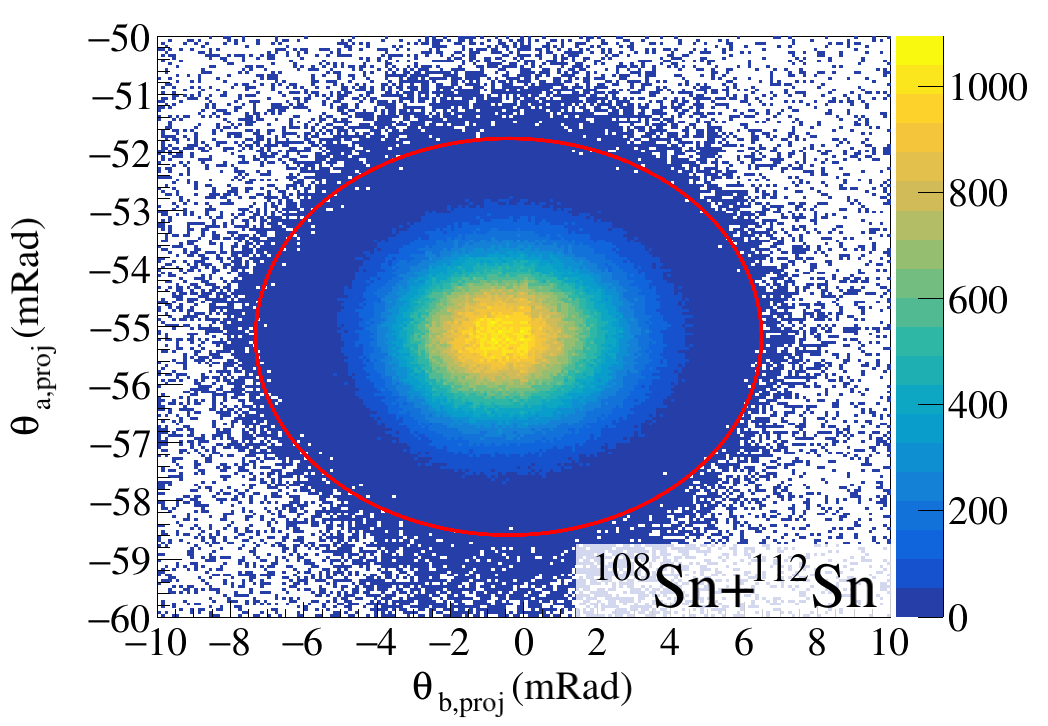
\includegraphics[width=\linewidth]{beamAngle-Sn108.png} 
        \caption{Beam angle of the $\tin{108}{124}$ system} \label{fig:beamangle108}
    \end{subfigure}
    \hfill
    \begin{subfigure}[t]{0.45\textwidth}
        \centering
        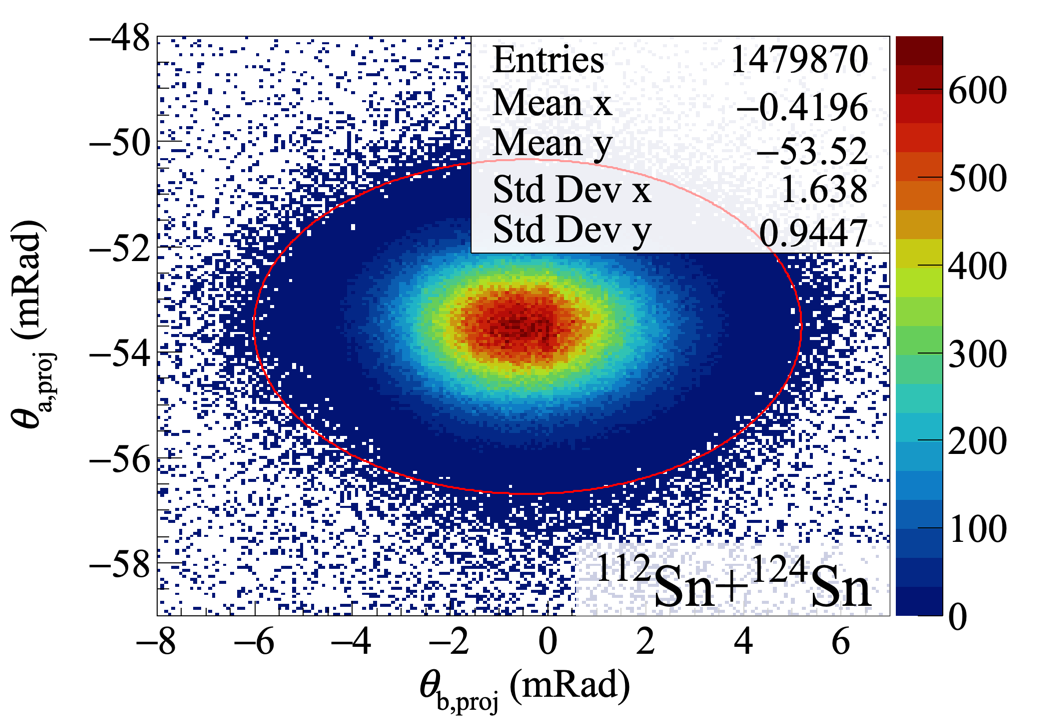
\includegraphics[width=\linewidth]{beamAngle-Sn112.png} 
        \caption{Beam angle of the $\tin{112}{124}$ system} \label{fig:beamangle112}
    \end{subfigure}
    
    \begin{subfigure}[t]{0.45\textwidth}
        \centering
        \includegraphics[width=\linewidth]{beamAngle-Sn124.png} 
        \caption{Beam angle of the $\tin{124}{112}$ system} \label{fig:beamangle124}
    \end{subfigure}
    \hfill
    \begin{subfigure}[t]{0.45\textwidth}
        \centering
        \includegraphics[width=\linewidth]{beamAngle-Sn132.png} 
        \caption{Beam angle of the $\tin{132}{124}$ system} \label{fig:beamangle132}
    \end{subfigure}
\label{fig:beamangle}
\end{figure}


Figure~\ref{fig:beamangle} shows the distribution of beam angles for ${}^{132}$Sn and ${}^{108}$Sn systems. Graphical cuts represented by the red lines where events lying in the cuts represent beams that were reconstructed correctly by the beam tracking software outlined in \cite{jon}. Helping to eliminate some of the poorly reconstructed beam events. 



\section{Vertex Cut}

\begin{figure}[!htb]
\centering
\includegraphics[scale =.5]{vertexDistribution.png}
\caption{Projection of the vertex onto the z-axis.}
\label{fig:overviewVertex}
\end{figure}


\begin{figure}[!htb]
\centering
    \begin{subfigure}[t]{\textwidth}
        \centering
        \includegraphics[width=\textwidth]{vertex-Sn108.png} 
        \caption{$\tin{108}{124}$ vertex distributon for all runs.} \label{fig:vertex108}
    \end{subfigure}
    \hfill
    \begin{subfigure}[t]{\textwidth}
        \centering
        \includegraphics[width=\textwidth]{vertex-Sn112.png} 
        \caption{$\tin{112}{124}$ vertex distributon for all runs.} \label{fig:vertex112}
    \end{subfigure}
    
    \begin{subfigure}[t]{\textwidth}
        \centering
        \includegraphics[width=\textwidth]{vertex-Sn124.png} 
        \caption{$\tin{124}{112}$ vertex distributon for all runs.} \label{fig:vertex124}
    \end{subfigure}
    \hfill
    \begin{subfigure}[t]{\textwidth}
        \centering
        \includegraphics[width=\textwidth]{vertex-Sn132.png} 
        \caption{$\tin{132}{124}$ vertex distributon for all runs.} \label{fig:vertex132}
    \end{subfigure}
\caption{}
\label{fig:vertexdist}
\end{figure}

The vertex information of an event, described in \ref{sec:vertex}, is estimated from reconstructing the tracks of an event to one common source. The secondary beam encounters several solid and gaseous materials were a nuclear reaction can occur anywhere along the beam line. Figure~\ref{fig:overviewVertex} shows the z component of the reconstructed vertex for all events in the ${}^{132}$Sn system. Several peaks are seen in the spectrum which correspond to several dense materials in the beam line such as the entrance windows, target frame, Active Veto, with the largest peak representing the target. Also collisions happen with the detector gas inside the TPC volume which are typically called active target events. To ensure that the secondary beam is really on the target of choice we perform a vertex cut around where we believe the vertex location of the target to be.
 
 The target position was measured to be \SI{-13.2}{\milli\metre}. The z-component of all runs in each beam type are plotted around the the target region in Fig.~\ref{fig:vertexdist}. The mean position of the vertex from the reconstructed data is around \SI{-14.76}{\milli\metre} which is about \SI{1.6}{\milli\metre} off from the expected target position. The mean position for each system is listed in Table~\ref{tb:vertexresol}. Since the target thickness was less than \SI{1}{\milli\metre} for all targets. Neglecting the small distributions in the thin target, the measured width of the vertex distribution can be interpreted directly as the vertex resolution of the TPC. The extracted vertex resolutions of each system are summarized in Table~\ref{tb:vertexresol}, with an average vertex resolution of \SI{1.2}{\centi\metre}. The difference between the measured and actual target location is 10 times smaller than the intrinsic vertex resolution of the detector and is really and insignificant difference.  



\begin{table*}\centering
\ra{1.3}
\begin{tabular}{@{}rrr@{}}\toprule
\multicolumn{3}{c}{Vertex Resolution}\\
\cmidrule{1-3}
System & Mean (cm) & Sigma (cm) \\
\midrule
$\tin{132}{124}$ & -14.79  & 1.2 \\
$\tin{124}{112}$ & -14.71  & 1.1 \\
$\tin{112}{124}$ & -14.78  & 1.2 \\
$\tin{108}{112}$ & -14.75  & 1.3 \\ 
\bottomrule
\end{tabular}
\caption{Summary of measured verticies and their resolution.}
\label{tb:vertexresol}
\end{table*}


\clearpage

\section{Impact Parameter Selection}

\begin{figure}[htb]
\centering
\includegraphics[scale=.5]{error_b_full.pdf}
\caption{Estimate of the impact parameter from the track multiplicity.}
\label{fig:impactPar}
\end{figure}

The impact parameter is a theoretical quantity defined as the distance, between two centers of colliding nuclei. Though there is no way to directly measure the impact parameter in an experiment, the track multiplicity can be indirectly related to the estimated impact parameter of a collision \cite{impactpar}. As discussed in Section \ref{sec:kyoto}, the Kyoto multiplicity array was used to experimentally trigger on central nuclear collision events. This is under the assumption that as the number of charged particles produced in collision is related to the overlap region of the two nuclei. This is best described by a spectator-participant model of nuclear collisions, where a large fraction of the participating nucleons in the overlap region of the two colliding nuclei fragment into individual and clusters of nucleons. In the case where the impact parameter is zero, all the nucleons in both nuclei participate, were as larger impact parameters -- more peripheral collisions -- less nucleons participate. 


%Certainly the Kyoto array introduces a bias in our measurement of the multiplicity of all the events. At low track multiplicities, the orientation of the event starts to play a major role. Theoretically the orientation of the event (the reaction plane) is random, but due to the fact that we only measure the multiplicity on the sides of the TPC, we are preferentially triggering on events with reaction planes that emit particles in these directions. Therefore events with low track multiplicity (therefore more peripheral), that emit preferentially up and down in the TPC will not be triggered on. This becomes less of an issue as even in mid-peripheral collisions were the number of particles emitted becomes much greater than the Kyoto multiplicity selection

The geometric cross section $\sigma$ can be described as, 

\begin{equation}
\sigma = \pi \cdot b^2,
\label{eq:crossSect}
\end{equation}

where $b$ is the impact parameter of the collision.  If the track multiplicity of an event $N_C$ is monotonically related to the cross section, the impact parameter can be written as a reduced impact parameter $\hat{b}$ as,
\begin{equation}
\hat{b} =  \frac{b}{b_{max}} = \int^{\infty}_{N_C} \frac{dP(N_C)}{dN_C} dN_C,
\end{equation}

where $b_{\mathrm{max}}$ represents the maximum impact parameter detected by the TPC, $b$ is the impact parameter of the vent,  and $dP(N_C/dN_C$ is the normalized multiplicity distribution \cite{reducedimpact}. The reduced impact parameter ranges from $\hat{b}=0$ for the most central collisions and to $\hat{b}=1$ for the most peripheral. A  detailed analysis was performed, determining the maximum cross section $\sigma_{max}$, for each system, in which $b_{\mathrm{max} = \sqrt{\sigma_{max}/\pi}}$. The detailed analysis is given in \cite{jon}. Figure~\ref{fig:impactPar} shows the estimated impact parameter for a given track multiplicity with the estimated error bands for each system. 

In the $\tin{132}{124}$ system the multiplicity cut was $N_C > 50$ corresponding to $\hat{b} = 0.4$ and $b = \SI{3.1}{\femto\metre}$. For the $\tin{108}{112}$ system the multiplicity cut was $N_C > 49$ corresponding to $\hat{b} = 0.4$ and $b = \SI{3.1}{\femto\metre}$. These values were averaged over the multiplicity distribution as,

\begin{equation}
 \overline{X} = \int_{N_C}^{\infty} X\frac{dP(N_C)}{dN_C} dN_C
\end{equation}

where X can be the variables $b$, $\hat{b}$. In the $\tin{132}{124}$ system the average $\overline{\hat{b}} = \num{.1(1)}$ and $\overline{b} = \SI{3}{\femto\metre}$. In the $\tin{108}{112}$ system the average $\overline{\hat{b}} = .1$ and $\overline{b} = \SI{3}{\femto\metre}$. These quantities are useful when comparing to theory. 

\section{Track Quality Cuts}
\label{sec:qualitycut}
%graphic showing distance to vertex, number of clusters
%number of cluster cut
%distance to vertex
In this section we will discuss cuts which address the quality of the reconstructed track, in the following we will simply refer this as the ``track quality". Assuming tracks are mostly continuous in clusters, i.e. only randomly missing a few clusters, the number of clusters is directly related to the momentum resolution of a track. Tracks with more clusters correspond to better PID and momentum resolution. Upward-going and downward-going tracks, at larger values of $\theta_{Lab}$ are limited by the vertical space of the TPC. In these regions the track length is short and there are few clusters which are reconstructed. This leads to the low efficiency in these regions as discussed earlier in Sec.~\ref{sec:efficiency}. A cut where tracks with the number of clusters $N_{cl} > 20$ are considered quality tracks. Later in Section~\ref{sec:cutvar} the exact choice of the number 20 is discussed in more detail.

\begin{figure}[!htb]
\centering
\includegraphics[scale=1.]{distancetovertex.pdf}
\label{fig:poca}
\caption{Distance to vertex for tracks.}
\end{figure}

For very long tracks, such as low momentum pions, which can make a complete circular path in the TPC, it can happen that the software incorrectly identifies the track as several separate tracks. This can happen due to discontinuities in the track due to missing hits from low energy loss, shadowing due to saturation, or possibly the software algorithm itself. Of course including all of the tracks would be counting the track several times over, and would lead to incorrect particle yields. The software will occasionally associate random disassociated clusters and construct a false track, or a so called ``ghost track". These type of tracks contribute to the background in the PID. In both of the situation of the false track or in the case of a split track the false track origin cannot be traced back to anywhere near the vertex of the event, and the distance-Of-Closest-Approach (dOCA) between the track and vertex is very large. 

To reduce the number of false tracks, a simple cut on the dOCA can be used. The vector representing the minimum distance to vertex for each track can be calculated and its corresponding magnitude. We define the distance to vertex cut as a small sphere centered around the vertex location with a some radius $R$. If the dOCA of a particular track $d_i < R$, the track is assumed to have originated from the vertex; tracks outside of the cut are thrown out of the analysis. 






\section{Angular Quality Cuts}

Since the TPC does not have spherical symmetry, there are geometric constraints and considerations that effect the efficiency of track reconstruction. Most notably upward and downward-going tracks will have the shortest track length and will correspond to low regions of efficiency as seen in \ref{sec:efficiency}. The relevant geometries which determine these regions are the corners of the field cage. Figure~\ref{fig:angleEffExplanation} shows a cartoon drawing of the front of the field cage were the angles of each corner is given. Since the window to the field cage was slightly higher, the upper angles are slightly smaller than the lower angles. These angles are actually the same as the spherical $\phi$ angle, where the left and right, most efficient regions, correspond to  $\ang{0}\substack{+24 \\ -34}$ and $\ang{180}\substack{+34 \\ -24}$.  While the exact area of zero efficiency depends on polar angle $\theta_{Lab}$, a clear cut off around these angles can be seen in Fig.~\ref{fig:angleEffExplanation} in the angular distribution of the measured tracks, where the experimental data was fitted with a Fermi distribution to find the inflection point of where the efficiency drops off significantly. The angular cuts applied to the data is listed by particle type in Table~\ref{tb:anglecuts}. The values are very similar to the simple calculation that was outlined above. 


\begin{figure}[!htb]
\centering
\includegraphics[scale=.75]{tpcAngle.pdf}
\caption{Rough Geometry of the TPC field cage.}
\label{fig:angleEffExplanation}
\end{figure}


\begin{figure}[!htb]
     \centering
     \begin{subfigure}[b]{0.49\textwidth}
         \centering
         \includegraphics[width=\textwidth]{angularCut-pim-Sn108.png}
         \caption{$y=x$}
         \label{fig:pim108angle}
     \end{subfigure}
     \hfill
     \begin{subfigure}[b]{0.49\textwidth}
         \centering
         \includegraphics[width=\textwidth]{angularCut-pim-Sn132.png}
         \caption{$\tin{132}{124}$ $\pi^-$ angular spectra.}
         \label{fig:pim132angle}
     \end{subfigure}
        \caption{Three simple graphs}
        \label{fig:pim}
\end{figure}


\begin{figure}[!htb]
     \centering
     \begin{subfigure}[b]{0.49\textwidth}
         \centering
         \includegraphics[width=\textwidth]{angularCut-pip-Sn108.png}
         \caption{$\tin{108}{112}$ $\pi^-$ angular spectra.}
         \label{fig:pip108angle}
     \end{subfigure}
     \hfill
     \begin{subfigure}[b]{0.49\textwidth}
         \centering
         \includegraphics[width=\textwidth]{angularCut-pip-Sn132.png}
         \caption{$\tin{132}{124}$ $\pi^-$ angular spectra.}
         \label{fig:pip132angle}
     \end{subfigure}
        \caption{Three simple graphs}
        \label{fig:pip}
\end{figure}



 \begin{table*}[!htb]
 \centering
\ra{1.3}
\begin{tabular}{@{}ccc@{}}\toprule 
Particle Type & $\theta_{CM}$ cut & $\phi$ cut  \\ [0.5ex] 
 \midrule
$\pi^+$  & $\theta_{CM}$ < \ang{90}   &  \ang{-35} < $\phi$ < \ang{20} $\cap$ \ang{157} < $\phi$ < \ang{219}  \\
$\pi^-$  & $\theta_{CM}$ < \ang{90}   &  \ang{-40} < $\phi$ < \ang{25} $\cap$ \ang{158} < $\phi$ < \ang{212}   \\
 \bottomrule
\end{tabular}
\caption{Angular cuts for each system and particle type}
\label{tb:anglecuts}
\end{table*}



These regions can also be seen in the earlier discussion in the MC embedded efficiency in Fig.~\ref{fig:pim_eff_ex}.  We could of course include a larger region where the efficiency is small but not zero but it is good practice not to efficiency correct already small numbers with small efficiency values. The solid angle covered by the cut is written as,

\begin{equation}
\Delta\Omega = \Delta\phi(\cos(\theta_1) - \cos(\theta_2)),
\end{equation}

where $\Delta\phi = (\phi_2 - \phi_1)$  and $\theta_{1,2}$ are the $\theta$ angle cuts, in units of \si{\radian}. The solid angle covered by the $\pi^-$ cuts is \SI{2.077}{\steradian} and for $\pi^+$ cuts \SI{2.042}{\steradian}. Assuming the pion emission is isotropic, we multiply each observed pion by a correction factor, $C_a$, to correct for the full 4$\pi$ angular coverage, 

\begin{equation}
C_a = \frac{4\pi}{\Delta\Omega},
\end{equation}

for $\pi^+$ that is \num{6.15} and $\pi^-$ \num{6.05}. We assume the pion emission is isotropic for a couple of reasons. The symmetry of very central collisions is invariant with respects to any rotations. Also the mass of the pion is smaller than the nucleons mass and therefore collective motion leading to anisotropies would be small for the pion, i.e. most of the motion would be thermal. We also measured two systems $\tin{112}{124}$ and its inverse $\tin{124}{112}$. The forward emission in the $\tin{124}{112}$ system is really the same as the backward emission of the $\tin{112}{124}$ system and vice versa. It was shown for pions emitted in central collisions the forward and backward emission was the same \cite{jon}, proving that at least for central collisions pions are emitted isotropically to a good approximation. 



\chapter{Results}
\section{Comparison to Theory}
Add figure of Pion spectra for different theory 
Reference paper for multiple theories
 
\section{Pion Spectra and Yields}
Add figure on Glauber model 
Add figure on comparison to FOPI data
Add figure of angular coverage of TPC spectra 

\section{$\pi^-$/$\pi^+$ Ratio}
Add figure of Theory for pion ratios

\section{Pion Double Ratio}
Add figure of Theory for pion ratios

\section{Constraint on the Symmetry Energy}
maybe not...




%
% If you have pages that must appear in landscape mode, use the [lscape] documentclass option
% and enclose the pages in a {landscape} environment.
%\clearpage\pagestyle{lscape} % first clear the page and change the pagestyle
%\begin{landscape}
%
% your landscape table(s) or figure(s) here
%
%\end{landscape}
%\pagestyle{plain} % remember to change the pagestyle back to plain
%
%
% If you have appendices, they would go here.  
% Comment these lines out if you don't
% If you have more than one appendix, you need to use 
%   \begin{appendices}
%   \chapter{First appendix}
%   \chapter{Second appendix}
%   \end{appendices}
%ch_nucleareos.txt~
\appendix
\chapter{Your appendix}
%
\backmatter
% The next lines add the dots back into the References/Bibliography heading
% of the TOC.  Only uncomment this if you need to put the dots back in having removed them for Chapter headings.
%
%\addtocontents{toc}{%
%   \protect\renewcommand{\protect\cftchapterdotsep} {\cftdotsep}}
%
\makebibliographypage % make the bibliography cover page
% Bibliography can be single spaced
%
\SingleSpacing
%
% Your bibliography command here (e.g. \bibliography{your-bib-file}) if using natbib
%
% Remember that although the bibliography is single spaced, there needs to
% be a blank line between entries. This is set by your bibliography package
% If you are using natbib it is \bibsep; if using biblatex it's \bibitemsep
\bibliography{mybibfile}

\end{document}

